\documentclass[a4paper,12pt,twoside]{mythesis}

\usepackage[T1]{fontenc}
\usepackage{lmodern}
\usepackage{listings}
\usepackage{dcolumn}
\usepackage{graphicx}
\usepackage{fancyhdr}
\usepackage[english, german]{babel}
\usepackage{xspace}
\usepackage[pdftex]{hyperref}
\usepackage{amsmath}
\usepackage{amssymb}
\usepackage{amsfonts}
\usepackage[obeyFinal,colorinlistoftodos,textsize=scriptsize,textwidth=0.3\textwidth]{todonotes}
\usepackage{rotating}
\usepackage{lscape}
\usepackage{longtable}
\usepackage{multirow}
\usepackage{colortbl}
\usepackage{triotex}
\usepackage{enumitem}
\usepackage[rightcaption]{sidecap}
\usepackage{caption}
\usepackage{changepage}

\usepackage{chngcntr}
\counterwithout{figure}{chapter}
\counterwithout{table}{chapter}


\newcommand{\AutoProof}{Auto\-Proof\xspace}
\newcommand{\AutoTest}{Auto\-Test\xspace}
\newcommand{\AutoFix}{Auto\-Fix\xspace}
\newcommand{\Inspector}{Eiffel Inspector\xspace}
\newcommand{\EVE}{EVE\xspace}
\newcommand{\VAssist}{Verification Assistant\xspace}
\newcommand{\VSRepo}{Verified Software Repository\xspace}

\renewcommand{\t}{\ensuremath{\mathcal{T}}\xspace}
\newcommand{\tr}[1]{\ensuremath{\mathcal{T}\ifx\\#1\\ \else(#1)\fi}}
\newcommand{\ts}[2]{\ensuremath{\mathcal{T}_{\mathrm{#1}}\ifx\\#2\\ \else(#2)\fi}}
\newcommand{\m}{\ensuremath{\mathcal{M}}\xspace}
\newcommand{\map}[1]{\ensuremath{\mathcal{M}\ifx\\#1\\ \else(#1)\fi}}


% from VSTTE paper
\newcommand{\sub}{\ensuremath{\mathsf{sub}}}
\newcommand{\inline}{\ensuremath{\mathsf{inline}}}
\newcommand{\unroll}{\ensuremath{\mathsf{unroll}}}
\newcommand{\paths}{\ensuremath{\pi}}
\newcommand{\insize}[1]{\ensuremath{\Vert#1\Vert}}

% Colors
\definecolor{darkred}{HTML}{990000}
\definecolor{darkgreen}{HTML}{007700}

% Automatic row numbers
\newcounter{tablerownumbers}
\newcommand\rownumber{\refstepcounter{tablerownumbers}\arabic{tablerownumbers}}

% Unique numbering of tables and figures (from stackoverflow)
% see http://bugcounting.net/blog/?p=99
\makeatletter
\renewcommand*{\thetable}{\arabic{table}}
\renewcommand*{\thefigure}{\arabic{figure}}
\let\c@table\c@figure
\makeatother

% Headings
\addtolength{\headwidth}{\marginparsep}
\addtolength{\headwidth}{\marginparwidth}
\lhead[\fancyplain{}{\thepage}]  {\fancyplain{}{\rightmark}}
\rhead[\fancyplain{}{\leftmark}] {\fancyplain{}{\thepage}}
\cfoot{}
\setlength{\headheight}{28pt}

%%%%%%%%%%%%%%%%%%%%%%%%%%%%%%%%%%%%%%%%%%%%%%%%%%%%%%%%%%%%%%%%%%%%%%%%%%%%%%
% CODE LISTINGS
%%%%%%%%%%%%%%%%%%%%%%%%%%%%%%%%%%%%%%%%%%%%%%%%%%%%%%%%%%%%%%%%%%%%%%%%%%%%%%

% Set up font
\usepackage[scaled=0.85]{beramono} 

% Eiffel language
\usepackage{eiffel}
\newcommand{\eiffel}[1]{\mbox{\lstinline[language=Eiffel]|#1|}}
\newcommand{\e}[1]{\mbox{\lstinline[language=Eiffel]|#1|}}
\lstnewenvironment{efigure}[3][]
{\figure[#1]\small\lstset{language=Eiffel}}
{\caption{#2}\label{#3}\endfigure}
\lstnewenvironment{erunning}[1][]
{\small\lstset{language=Eiffel, numbers=none, #1}}{}

% Boogie language
\usepackage{boogie}
\newcommand{\boogie}[1]{\mbox{\lstinline[language=Boogie]|#1|}}
\renewcommand{\b}[1]{\mbox{\lstinline[language=Boogie]|#1|}}
\lstnewenvironment{bfigure}[3][]
{\figure[#1]\small\lstset{language=Boogie}}
{\caption{#2}\label{#3}\endfigure}
\lstnewenvironment{brunning}[1][]
{\small\lstset{language=Boogie, numbers=none, #1}}{}

%%%%%%%%%%%%%%%%%%%%%%%%%%%%%%%%%%%%%%%%%%%%%%%%%%%%%%%%%%%%%%%%%%%%%%%%%%%%%%
% CHAPTER IMAGES
%%%%%%%%%%%%%%%%%%%%%%%%%%%%%%%%%%%%%%%%%%%%%%%%%%%%%%%%%%%%%%%%%%%%%%%%%%%%%%

\usepackage{grfext}
\PrependGraphicsExtensions*{.png,.PNG}

% switch
\newif\ifprintimage
\printimagetrue

% image function
\usepackage[absolute]{textpos}
\newcommand{\chapterimage}[1]{
\begin{textblock*}{\paperwidth}(0mm,60mm)
\ifprintimage
  \includegraphics[width=\paperwidth,height=0.5\paperheight]{#1}
\fi
\end{textblock*}
}

% title color and font
\definecolor{title}{HTML}{00AEEF}
\usepackage{transparent}
\newcommand\customfont[1]{{\usefont{T1}{custom}{m}{n} #1 }}

% title adaptations
\usepackage{titlesec}
\newcommand{\normalchapter}{
  \titleformat{\chapter}[display]
    {\normalfont\Huge\scshape}
    {\chaptertitlename\ \thechapter}
    {20pt}
    {\Huge}
  \titlespacing*{\chapter}{0pt}{50pt}{40pt}
}
\newcommand{\imagechapter}{
  \ifprintimage
    \titleformat{\chapter}[display]
      {\normalfont\Huge\scshape\color{title}\usefont{T1}{custom}{m}{n}}
      {\chaptertitlename\ \thechapter}
      {140pt}
      {\scriptsize\transparent{0}}
    \titlespacing*{\chapter}{0pt}{-25pt}{300pt}
  \fi
}
%\titleformat{\section}
%  {\normalfont\Large\bfseries\color{title}\usefont{T1}{custom}{m}{n}}{\thesection}
%  {1em}
%  {}
\normalchapter

%%%%%%%%%%%%%%%%%%%%%%%%%%%%%%%%%%%%%%%%%%%%%%%%%%%%%%%%%%%%%%%%%%%%%%%%%%%%%%
% DOCUMENT
%%%%%%%%%%%%%%%%%%%%%%%%%%%%%%%%%%%%%%%%%%%%%%%%%%%%%%%%%%%%%%%%%%%%%%%%%%%%%%
\begin{document}

\frenchspacing
\selectlanguage{english}

  \pagenumbering{alph}\pagestyle{empty}

%\begin{textblock*}{\paperwidth}(0mm,0mm)
   \noindent
\includegraphics[width=\paperwidth]{images/coverpage}
\end{textblock*}
\mbox{}
 \cleardoublepage
\mbox{}

%\vskip 0.5cm

\centerline{\sc Diss. ETH No. 22463}

\vskip 1cm

\begin{center}
\huge \textbf{Automated Usable\\ Functional Verification of\\ Object-Oriented Programs}
\end{center}

\vskip 1cm

\centerline{\it A thesis submitted to attain the degree of}

\vskip 0.5cm

\centerline{DOCTOR OF SCIENCES of ETH ZURICH}
\centerline{(Dr. sc. ETH Zurich)}

\vskip 1.0cm

\centerline{\it presented by}
\centerline{JULIAN MARTIN TSCHANNEN}
\centerline{MSc ETH in Informatik, ETH Z\"urich, Switzerland}
\vskip 0.5cm

\centerline{\it born on}
\centerline{October 27th, 1982}

\vskip 0.5cm

\centerline{\it citizen of}
\centerline{Wohlen bei Bern, BE}

\vskip 1.0cm

\centerline{\it accepted on the recommendation of}
\vskip 0.5cm
\centerline{Prof. Dr. Bertrand Meyer, examiner}
\centerline{Prof. Dr. Marsha Chechik, co-examiner}
\centerline{Dr. Carlo A. Furia, co-examiner}
\centerline{Dr. Francesco Logozzo, co-examiner}
\centerline{Prof. Dr. Jim Woodcock, co-examiner}

\vskip 1.0cm

\centerline{2015}
 \cleardoublepage

  \pagenumbering{roman}\pagestyle{plain}

\normalchapter
\chapter*{Acknowledgments}
%\chapterimage{images/acknowledgments.jpg}


%1. Bertrand Meyer

I thank Bertrand Meyer for giving me the opportunity to do a PhD at ETH Zurich.
His support and the programming language he created were the foundation of this work.

%2. Martin Nordio and Carlo A. Furia

Also, this dissertation would not have been possible without the help and supervision of Martin Nordio and Carlo A. Furia.
Their expertise and feedback was invaluable for my progress.

%3. Nadia Polikarpova and Christian Estler

A direct impact to this work also comes from Nadia Polikarpova, who designed an awesome framing methodology and was a co-developer of \AutoProof during its recent stages, and Christian Estler, who put \AutoProof on the web.

%4. Co-supervisors

Additionally I thank my co-examiners Marsha Chechik, Carlo A. Furia, Francesco Logozzo, and Jim Woodcock for evaluating my dissertation.

%5. Coworkers

My time in this research group was very enjoyable thanks to all the wonderful co-workers:
 Andrey Rusakov,
 Benjamin Morandi,
 Carlo A. Furia,
 Chandrakana Nandi,
 Christian Estler,
 Claudia G\"unthart,
 Cristiano Cal\-ca\-gno,
 \DH urica Nikoli\'{c},
 Georgiana Caltais,
 Jason (Yi) Wei,
 Jiwon Shin,
 Marco Piccioni,
 Marco Trudel,
 Martin Nordio,
 Max (Yu) Pei,
 Michela Pedroni,
 Mischael Schill,
 Roman Schmocker,
 Scott West,
 Sebastian Nanz,
 Stephan van Staden.

%6. People at Eiffel Software

I also thank Manu Stapf from Eiffel Software, who speedily replied whenever I had a question about EiffelStudio.

%7. Family and Friends

During my studies at ETH and before I found wonderful friends with whom I had and continue to have a great time: 
 Antoni Amerena,
 Antonio Barresi,
 Till Bay,
 Nicola Chiapolini,
 Urs D\"onni,
 Bruno Hauser,
 Sven Mader,
 Lukas Naef,
 Tahmineh Sanamrad,
 Martin Seiler,
 Valentin W\"ustholz.

Lastly I thank my family, who supported me on my journey all my life, and in particular my wife Maria Gubar (aka \emph{LimKis}), who designed the amazing cover page and illustrations.


 \cleardoublepage
\tableofcontents\cleardoublepage
\chapter*{Abstract}
%\chapterimage{images/abstract1.jpg}

% Automated Usable Functional Verification of Object-Oriented Programs
% ====================================================================
% 1. What is the problem? 
%		Verifying object-oriented programs is difficult for average programmers
% 2. Why is this problem interesting/relevant?  
% 		OO is widespread, advanced verification techniques help to improve software quality
% 3. What is our solution approach? 
% 		techniques for usable auto-active verification
% 		implemented in an auto-active verifier for Eiffel
% 		combining different verification and analysis tools
% 4. What did we achieve? 
% 		AutoProof, an auto-active verifier for Eiffel, that is capable of verifying challenging OO patterns and algorithmic problems, evaluated on a suite of verification challenges
% 		A verification assistant that combines three completely different tools to support programmers focus on important areas of the code-base



Object-oriented programming is pervasive in today's software world; languages based on object-orientation are used from small devices to large projects.
Yet, automatic verification of object-oriented programs mostly uses dynamic approaches such as testing.
In this thesis we focus on two aspects to improve this situation: (1) supporting full functional verification of object-oriented programs and (2) automated techniques to make verification of object-oriented programs more usable. To attain these goals we have developed several methodologies for automated verification, built an automated verifier, and developed a high-level technique to combine multiple tools in an IDE.

Software developers nowadays can choose from many different tools for analyzing and verifying their code using different techniques both static and dynamic.
These tools usually have independent interfaces and may force the programmer to explicitly switch tasks when working with them.
We have developed a scoring system to make the process of using several tools in combination more streamlined.
Several tools work in the background side by side while an aggregator collects the results and displays a combined score based on the individual results.
This frees the developer from invoking tools and unifying the results manually to get the full picture of the state of the program.
To demonstrate the technique we built the \VAssist combining three tools: a static verifier (\AutoProof), a dynamic verifier (\AutoTest), and a light-weight code checker (\Inspector).

With \AutoProof we have built a state-of-the-art automated verifier for object-oriented sequential programs with complex functional specifications. \AutoProof incorporates two-step verification among other techniques such as semantic collaboration and agent verification. To show \AutoProof's performance on verifying object-oriented idioms as well as standard algorithmic problems, we have made an evaluation of \AutoProof on a rich collection of benchmark problems from recent verification competitions.
The results attest \AutoProof's competitiveness among tools in its league on cutting-edge object-oriented verification problems.

To improve feedback of failed verification attempts, we have developed \emph{two-step verification}, a technique that combines implicit specifications, inlining, and loop unrolling.
Two-step verification performs two independent verification attempts for each program element: one using standard modular reasoning, and another one after inlining and unrolling; comparing the outcomes of the two steps suggests which elements should be improved.

Both our tools---\AutoProof and the \VAssist---are available in \EVE, the open-source Eiffel Verification Environment. Additionally, \AutoProof is available through an on-line interface together with a tutorial, user manual, and a repository with all our solutions to benchmark problems.



\chapter*{Zusammenfassung}
%\chapterimage{images/abstract2.jpg}

\selectlanguage{german}

Objekt-orientierte Programmierung ist in der heutigen Softwarewelt allgegenw\"artig; Sprachen die auf objekt-orientierung aufbauen werden von kleinen Ger\"aten bis zu grossen Projekten verwendet.
Trotzdem wird in der Verifikation von objekt-orientierten Programmen haupts\"achlich dynamische Ans\"atze wie zum Beispiel \emph{Testen} angewendet.
In dieser Doktorarbeit fokussieren wir uns auf zwei Aspekten um diese Situation zu verbessern: (1) volle funktionale Verifikation von objekt-orientierten Programmen und (2) automatische Techniken, welche die Verifikation von objekt-orientierten Programmen benutzerfreundlicher machen.
Um diese Ziele zu erreichen haben wir mehrere Methoden f\"ur automatisierte Verifikation entwickelt, einen automatisierten Verifizierer implementiert und eine Technik entwickelt, um mehrere Tools in einer IDE auf hoher Abstraktionsstufe zu kombinieren.

Softwareentwickler k\"onnen heutzutage von einer Vielzahl von Tools f\"ur die Analyse und Verifikation ihre Codes w\"ahlen, sowohl Tools die statische als auch dynamische Techniken verwenden.
Diese Tools k\"onnen eigene Benutzeroberfl\"achen anbieten und zwingen so den Programmierer explizit mit diesen Tools zu interagieren.
Wir haben ein Punktesystem entwickelt, das die Benutzung mehrere Tools in Kombination vereinfachen soll.
Mehrere Tools arbeiten im Hintergrund Seite an Seite, w\"ahrend ein Aggregator die Resultate sammelt und eine kombinierte Punktezahl basierend auf den individuellen Resultaten anzeigt.
Dies befreit den Entwickler davon, die Tools einzeln zu verwenden, und die Resultate manuell zu kombinieren um sich ein Bild vom Zustand des Programms zu machen.
Um diese Technik zu demonstrieren haben wir den \VAssist entwickelt, der drei Tools kombiniert: einen statischen Verifizierer (\AutoProof), einen dynamischen Verifizierer (\AutoTest), und einen leichtgewichtigen Code-Pr\"ufer (\Inspector).

Mit \AutoProof haben wir einen modernen auto-aktiven Verifizierer f\"ur sequentielle objekt-orientierte Programme mit komplexen funktionalen Spezifikationen entwickelt.
\AutoProof unterst\"utzt Zwei-Phasen Verifikation und andere Techniken wie Semantische Kollaboration und Verifikation von Agenten. Um die Leistung von \AutoProof bei der Verifikation von objekt-orientierten Idiomen und auch algorithmischen Problemen aufzuzeigen, haben wir eine Evaluation von \AutoProof auf einem vielf\"altigen Benchmark von Problemen k\"urzlicher Verifikations-Wettbewerbe gemacht.
Die Resultate attestieren die Konkurrenzf\"ahigkeit von \AutoProof gegen\"uber anderen Tools in seiner Liga bei aktuellen objekt-orientierten Verifikationsproblemen.

Um das Feedback bei fehlgeschlagenen Verifikationsversuchen zu verbessern haben wir \emph{Zwei-Phasen Verifikation} entwickelt; eine Technik, welche implizite Spezifikationen, Inlining und Loop Unrolling kombiniert.
Zwei-Phasen Verifikation f\"uhrt zwei unabh\"angige Verifikationsversuche durch f\"ur jedes Programmelement: die erste Phase benutzt das modulare Verfahren und die zweite Phase verifiziert nach Inlining und Unrolling. Der Vergleich dieser beiden Phasen weist auf das Programmelement hin, welches zu verbessern ist.

Unsere beiden Tools---\AutoProof und der \VAssist---sind in \EVE integriert, dem quelloffenen Eiffel Verification Environment. Zus\"atzlich ist \AutoProof \"uber eine online Benutzeroberfl\"ache erh\"altlich, zusammen mit einem Tutorial, einem Benutzerhandbuch und einem Archiv mit unseren L\"osungen zu Benchmark-Problemen.


\selectlanguage{english}
 \cleardoublepage

  \pagenumbering{arabic}\pagestyle{fancyplain}

\imagechapter
%############################################################################
\chapter{Introduction}
\label{sec:intro}
\chapterimage{images/introduction}
%############################################################################

%scoping
%- talk about the big problem
%- talk about individual issues, pointer to related work, short summary what we do, and point to individual chapters


%============================================================================
\section{Motivation and Goals}
%============================================================================

% what is the big problem?
% - software correctness is important
% - tools are important for software verification
% - to be more usable, tools need to be integrated in the software process, i.e. ide used by developers
% - to be more widely applicable, tools need to support idiomatic code and be scalable


Even long-standing skeptics must acknowledge the substantial progress of formal methods in the last decades.
Established verification techniques, such as those based on axiomatic semantics or abstract interpretation, have matured from the status of merely interesting scientific ideas to being applicable in practice to realistic programs and systems.
Novel approaches have extended the applicability of these techniques beyond their original scope, providing new angles from which to attack the hardest verification challenges; for example, model checking techniques, initially confined to digital hardware verification, are now applied to software or real-time systems.
Tool support has tremendously improved in terms of both reliability and performance, as a result of cutting-edge engineering of every component in the verification tool-chain as well as the increased availability of computing power.
Tools have practically demonstrated the impact of general theoretical principles, and they have brought automation into significant parts of the verification process.

%1. practical usage of oo
%oo patterns, polymorphism, exceptions, function objects, collaborative structures, modular design of programs (encapsulation, information hiding) to build large systems based on libraries
In modern object-oriented programming languages, developers write idiomatic object-oriented code based on established design patterns and using language features such as polymorphism, function objects, and exceptions.
Large systems are built based on modularity, encapsulation, and information hiding.
%2. functional verification
%specifications, design by contract. different tools available from code analysis through manual and automated testing frameworks to interactive and automated static verification tools
To provide automated verification of functional correctness of object-oriented programs, developers need to provide machine-readable specifications.
To this end, Design by Contract~\cite{MEYER92} has been adopted by several object-oriented programming languages, either natively~\cite{MEYER97,AMEER07} or ad-hoc~\cite{BARNETT10,LEAVENS05}.
This paves the way for tools to offer advanced code analysis, automated test generation, and static verification.

%3. challenge of 1.
%requires extensive specifications and advanced methodologies to deal with framing, aliasing, function objects, class invariants, collaboration; needs to be modular for scalability
Verification of idiomatic object-oriented code faces many challenges created by the flexibility offered to developers, such as framing, aliasing, class invariants, and collaborative object structures.
Large systems are built up from smaller components, encouraging modularity also on the level of verification.
%4. challenge of 2.
%needs to be usable in practice; it is possible to integrate multiple analysis or verification tools on different levels; to be open for future development of new tools, integration should be flexible
For developers to use verification tools in practice, tools need to be usable and cover a large part of the programming language.
With the advance in verification techniques, the number of tools available to developers is increasing as well.
Instead of just using these tools individually, integrating multiple tools in beneficial ways is a challenge as well, that can be addressed on different levels.

%5. thesis
%goal is to advance the state of the art in (1) proposing a novel way to combine verification tools (2) provide tool support for formal verification of idiomatic object-oriented programs (3) improve usability of verification tools
This is where this thesis tries to advance the state of the art: our goals are (1) to propose a novel way of integration verification tools, (2) provide tool support for formal verification of an object-oriented language, and (3) improve the usability of verification tools.



%============================================================================
\section{Summary and Main Results}
%============================================================================

% issue1: verification tool integration
% - developers have many different and diverse verification tools available
% - integration in IDEs is often limited to offering to use tools side-by-side, some frameworks offer integrated approaches
% - our approach is to use a verification assistant that
%   - runs automatic verification tools in the background
%   - automation and aggregation of results in a unified interface
%   - aggregates the results using a scoring system based on correctness confidence
%   - works on a high level and is therefore flexible to add or remove tools (good for research where tools might change quickly)

\subsection{Integration of verification tools}

With the increased availability of verification tools, developers have to integrate these tools into the development process.
To provide direct integration into the workflow of programmers, tools need to be available as part of the development environment (IDE).
Verification tools sometimes offer a standalone graphical user interface (e.g.~\cite{CUOQ12,FILLIATRE13}) or are integrated only loosely into an existing IDE (e.g.~\cite{BARNES03,COK11,LOGOZZO12}). In modern IDEs, multiple such tools are usually available side-by-side~\cite{VISUALSTUDIO,SPARKPRO,EIFFELSTUDIO}.
Different approaches have been proposed to leverage the existence of multiple tools by combining them in ways to enhance the individual functionalities, for example by combining multiple analyses~\cite{CORRENSON12}, making assumptions explicit~\cite{CHRISTAKIS12}, or by combining static and runtime verification~\cite{AHRENDT12}.
These integration techniques work on a low level and require the verification tools to be directly compatible in some form, therefore they are not applicable to integrate tools of widely differing techniques.

We propose an approach to combine the output of verification tools that works on a higher level of abstraction than existing techniques.
The integrated verification tools work completely independently and report their result to a central controller.
Each individual tool's results are summarized as a single correctness score for each unit of code (e.g. routine). In addition, tools report the confidence they have in their own score. The confidence is based on the tool's applicability to the verified code; for example, when a tool verifies a routine that uses floating-point arithmetic, but does not model floating-point numbers according to the underlying machine semantics, the confidence in the result will not be 100\%.
The controller then combines scores from different tools using weighted averages based on the confidence of each tool and other measures, e.g. visibility of routines.
Their aggregated results are displayed to the developer in a single interface, highlighting which areas of the program are in a good or bad shape with respect to the verification effort.
The advantage of working at this level of abstraction is that the integration is tool-agnostic:
The approach can be used to combine different tools that are completely independent from each other, supports integration of tools that use very different techniques, and simplifies the addition of new tools.
We have implemented this methodology in the \VAssist as part of the Eiffel Verification Environment (\EVE)~\cite{EVE} combining three diverse tools: (1) \AutoProof~\cite{TSCHANNEN15}, a static verifier; (2) \AutoTest~\cite{MEYER09}, an automatic contract-based testing tool; and (3) \Inspector~\cite{ZURFLUH14}, a light-weight code analysis tool.



% issue2: tool support for verification of an object-oriented language
% - object-oriented code poses specific challenges to handle aspects like object consistency, inheritance, and collaboration
% - diverse range of approaches exists based on different techniques like abstract interpretation or model checking
% - also deductive verification using proof assistants or smt solvers
% - we have chosen to follow the approach of deductive verification using Boogie as an intermediate verification language, similar to JML and Spec#, to verify Eiffel programs
%   - we have developed AutoProof, an auto-active verifier for Eiffel based on Boogie
%   - it supports verification of advanced object-oriented concepts: class invariants (including collaboration), agents, and inheritance
%   - we give detailed evaluation of using AutoProof on problems from recent verification competitions; we have used AutoProof to verify different algorithms 
%   - AutoProof has been used in a verification course to introduce students to software verification

\subsection{Verification of object-oriented programs}

Object-oriented programs pose many challenges to verification: accurately modeling heap manipulations in the presence of aliasing, object consistency, or inheritance while still having automated reasoning.
Different verification techniques like abstract interpretation~\cite{COUSOT77,COUSOT79}, model checking~\cite{CLARKE81}, or deductive verification~\cite{HOARE69} can be used to tackle these challenges.
While each technique offers different advantages as discussed in Section~\ref{sec:intro:related}, we have chosen to use the approach used by several other verifiers~\cite{BARNETT05,COHEN09,LEINO10,LEINO10c,COK11} and use Boogie~\cite{LEINO08} as an intermediate verification language.
The use of Boogie as an intermediate verification language allows us to work on a high level of abstraction when reasoning about the semantics of the programming language, Eiffel in our case, and makes sound and precise reasoning about complex properties possible.
In addition, using an intermediate verification language allows us to benefit from independent improvements on any element of the tool-chain.

Program verification techniques differ wildly in their degree of automation, ranging from completely \emph{automatic}, where the only input required is the program to be verified, to \emph{interactive} approaches to verification, where the user is ultimately responsible for providing input to the prover on demand.
In more recent years a new class of approaches have emerged that try to achieve an intermediate degree of automation between automatic and interactive---hence their designation~\cite{LEINO10b} as the portmanteau \emph{auto-active}\footnote{Although \emph{inter-matic} would be as good a name.}.
Auto-active tools need no user input during verification, which proceeds autonomously until it succeeds or fails; however, the user is still expected to provide guidance indirectly through \emph{annotations} (such as loop invariants) in the input program.
The auto-active approach has the potential of better supporting \emph{incrementality}: proving simple properties would require little annotations and of the simple kinds that novice users may be able to provide; proving complex properties would still be possible but by sustaining a high annotation burden.

With \AutoProof we developed an auto-active verifier for the Eiffel programming language. The verifier covers a large part of the Eiffel language and can be used to verify challenging problems. Practical verification of idiomatic object-oriented code is achieved by supporting methodologies such as semantic collaboration~\cite{POLIKARPOVA14}---a powerful methodology for framing and class invariants---and verification of function objects~\cite{NORDIO10}.
\AutoProof has been used to successfully verify a general-purpose container library~\cite{POLIKARPOVA15} and to verify client code that uses said library~\cite{FURIA15}.
We have evaluated \AutoProof on challenging examples, all of which are available online~\cite{APREPO}, that attest \AutoProof's competitiveness among other tools in its league.
We provide an in-depth discussion of a variety of challenges from recent verification competitions in Chapter~\ref{sec:eval}, describing in detail how \AutoProof performs on these examples.
\AutoProof is available for download as part of the Eiffel Verification Environment (\EVE)~\cite{EVE} or online on Comcom~\cite{APCOMCOM}. The usage is supported by a tutorial~\cite{APTUTORIAL} and a manual~\cite{APMANUAL} which are present in the Appendices~\ref{sec:ap-tutorial} and~\ref{sec:ap-manual}.



% issue3: auto-active verification of object-oriented code
% - Verifiers combine a variety of methodologies: framing, invariants, ...
% - our verifier incorporates different approaches that have been proposed by others
% - we also propose some methodologies usable by auto-active verifiers
%   - two-step verification
%   - polymorphic calls
%   - verification of eiffel exception handling

\subsection{Verification methodologies}

When developing a verifier for an object-oriented programming language, a crucial design choice are the supported verification methodologies.
For example, different approaches to framing (e.g.~\cite{REYNOLDS02,KASSIOS06}), dealing with class invariants (e.g.~\cite{BARNETT04,LEINO04,POLIKARPOVA14}), or dealing with function objects (e.g.~\cite{MUELLER09,NORDIO10}) have been proposed, including our own.
As part of our work with \AutoProof, we have developed new methodologies dealing with specific issues of verifying object-oriented code usable by auto-active verifiers:
\begin{itemize}
\item
One issue of a failed verification is that an auto-active prover does not indicate if the implementation has a fault or if the specification is too weak or strong.
A verification debugger allows developers to manually inspect the state of the verification~\cite{GOUES11} to gain insight into the underlying problem of the failed verification.
We propose a different approach that can in some cases automatically determine if the implementation or specification is to blame for a failed verification.
Our approach works by doing an additional verification step after a failed verification while inlining routine calls and unrolling loops.
With the information of both verification runs we can try to narrow down the possible reasons for the failed verification.
If the second verification attempt is successful, ignoring the specifications of routines and loops, this suggests that the implementation is correct and the specification should be adapted. We call this approach \emph{two-step verification} and use it to improve the feedback after a verification fails in \AutoProof.

\item
In object-oriented programming, subclasses can adapt the specification of routines by weakening the precondition and strengthening the postcondition.
However, verifiers tend to simplify this aspect and in general only take static types into consideration, limiting the precision of the verification.
We propose to use uninterpreted functions for pre- and postconditions and then linking the actual contracts of a routine to these uninterpreted functions based on the dynamic type of an object. With this approach, implemented in \AutoProof, a verifier can use contracts of the dynamic type for verification. This improves the precision of program verifiers when the dynamic type of an object can be inferred at a program location that uses a different static type.

\item
Verifying code that can throw exceptions introduces particular challenges.
When an exception is propagated to the caller, the regular postcondition is in general not established.
To address this issue, other verifiers offer two kinds of postconditions wherever necessary~\cite{MARCHE05,COK11}: a postcondition for case when the routine exits normally and a postcondition for the exceptional case.
Eiffel's peculiar exception mechanism introduces an additional problem on top of that by allowing to restart the execution of a routine in the case of an exception, which is akin to an implicit loop.
To verify Eiffel routines that trigger exceptions, we propose a solution that requires additional annotations analogous to loop invariants for the implicit loop introduced by the exception mechanism.
We have developed a methodology to annotate Eiffel code that uses exceptions and a translation to an intermediate verification language suitable for implementation in a verifier.
The methodology is not implemented in \AutoProof, since the Eiffel compiler that \AutoProof is built upon implements an old Eiffel exception mechanism, and we have used the Eiffel exception mechanism as proposed in the Eiffel ECMA standard~\cite{ECMA367} as a basis for the methodology.

\end{itemize}



%############################################################################
\subsection{Overview of Contributions}
%############################################################################

This thesis makes the following contributions:

%----------------------------------------------------------------------------
\subsubsection{Design of an integrated verification environment~\cite{TSCHANNEN11}}
%----------------------------------------------------------------------------

We have developed an approach to integrate verification tools in an IDE, resulting in an \emph{integrated verification environment}.
The high-level approach produces correctness scores for each routine and class, based on a combination of correctness scores of individual tools, confidence in the tool's results, and other factors such as importance of routines.
We have implemented this method in the \VAssist as part of the Eiffel Verification Environment.


%----------------------------------------------------------------------------
\subsubsection{Auto-active verification of Eiffel~\cite{TSCHANNEN15,TSCHANNEN14}}
%----------------------------------------------------------------------------

We have developed \AutoProof, an auto-active verifier for Eiffel.
The verifier covers a large part of the Eiffel language and can be used to verify challenging problems by supporting semantic collaboration~\cite{POLIKARPOVA14} and verification of function objects~\cite{NORDIO10}.
\AutoProof has been used to verify a general-purpose container library~\cite{POLIKARPOVA15}, verify client code of said library, as well as for teaching in a verification course~\cite{FURIA15}.
We discuss in-depth how \AutoProof verifies challenging examples and provide an online repository of examples verified with \AutoProof.
\AutoProof is integrated in the Eiffel Verification Environment and available through a web interface.


%----------------------------------------------------------------------------
\subsubsection{Methodologies for auto-active verification~\cite{TSCHANNEN13,TSCHANNEN12}}
%----------------------------------------------------------------------------

We introduce, implement, and evaluate on realistic examples several general methodologies usable by auto-active verifiers.

\begin{itemize}
\item
\emph{Two-step verification}, a technique to improve the feedback of failed verifications by doing a second verification step that uses inlining and unrolling.

\item
A methodology to use contracts of the dynamic type whenever the verifier can infer the dynamic type at a program location.

\item
A methodology to annotate and verify Eiffel code that uses exceptions.

\end{itemize}





%############################################################################
\section{Related Work}\label{sec:intro:related}
%############################################################################

%huge body of work exists in verification
%we focus on a few specific things
%  - working towards making verification a standard part of software engineering, IDE support
%  - Eiffel
%  - integration of verification in EVE
%  - deductive verification of Eiffel

A large amount of research exists in the area of software verification.
The work in this thesis falls in a subset outlined by the following criteria:
\begin{itemize}
\item
Functional verification of object-oriented programs equipped with contracts, including object-oriented idioms like inheritance and collaborative structures.

\item
Automated verification using an intermediate verification language based on deductive verification.

\item
Integrating different automated verification tools in an IDE, providing a unified interface.

\end{itemize}
This section discusses related work for each of these three general areas.
Later chapters contain additional related work sections focusing on more specific topics.


%----------------------------------------------------------------------------
\subsubsection{Programming Languages With Support for Verification}
%----------------------------------------------------------------------------

Verifying correctness of programs written in a general-purpose programming language is a daunting task.
To tackle automated verification of functional properties, a specification and the semantics of a programming language needs to be expressible in machine-readable form as well.
Some programming languages have been designed with support for specifications, others have support added on top of the language through comments, language extensions, or embedded through existing language mechanisms.
The following is a non-exhaustive list of programming languages with support for verification.

\paragraph{Boogie}

Boogie~\cite{LEINO08} is both an imperative programming language and a verifier.
The language supports first-order logic specifications and the definition of logic theories.
The verifier takes a Boogie program and generates verification conditions that can be discharged by SMT solvers such as Z3~\cite{MOURA08} or Simplify~\cite{DETLEFS05}.
Boogie has been used as an intermediate verification language for a number of verifiers, e.g. \AutoProof, Dafny~\cite{LEINO10}, or VCC~\cite{COHEN09}.
We use the Boogie language to model and verify the Eiffel language by mapping the object-oriented semantics to a procedural representation.

\paragraph{CodeContracts}

CodeContracts~\cite{BARNETT10} offers embedded contracts for the .NET platform through a contract library that allows one to express the specifications as part of the program.
Developers call the contract library's methods for different types of specifications such as pre- and postconditions, and write the specifications as arguments to these methods.
The CodeContracts framework supports both static checking and runtime monitoring of assertions~\cite{FAEHNDRICH10} (the latter through a post-build instrumentation step).
While CodeContracts offer the full range of specifications---including class invariants and contracts for abstract classes---through method annotations, the CodeContracts Checker~\cite{LOGOZZO12} focuses on properties verifiable without additional annotations, and does not target complex inter-dependencies idiomatic in some object-oriented patterns.
\AutoProof takes a different angle, focusing on the verification of complex properties including class invariants and aliasing.
This requires users of \AutoProof to provide more extensive annotations.

\paragraph{Dafny}

The Dafny~\cite{LEINO10} language and verifier were designed to work with specifications based on dynamic frames~\cite{KASSIOS06}.
Dafny has built-in support for contracts and allows the use of ghost code, making it possible to write expressive specifications.
Verification is achieved through a translation to Boogie and Dafny programs can be executed by generating .NET code.
Dafny is well-suited to verify algorithmic problems, but it does not support object-oriented concepts used in mainstream languages, for example inheritance.

\paragraph{Eiffel}

In our work we have used Eiffel~\cite{MEYER97}, a general-purpose object-oriented programming language that offers embedded contracts and user-defined annotations.
Since Eiffel has support for contracts since its creation, Eiffel programmers are familiar with writing contracts~\cite{ESTLER14}.
More recent versions of the Eiffel language have added support for loop expressions, which can be leveraged to express bounded quantification in assertions.
One of the underlying goals of this thesis is to work towards supporting the static verification of the full Eiffel language.

\paragraph{JML}

The Java Modeling Language (JML)~\cite{LEAVENS05} is a specification language for Java.
Contracts are expressed through special comments in the source code.
Multiple verifiers exist that work on Java programs annotated with JML, for example KeY~\cite{BECKERT07}, ESC/Java2~\cite{COK05,CHALIN06}, Krakatoa~\cite{FILLIATRE07}, and OpenJML~\cite{COK11}.
These tools focus on simpler properties and do not offer much support for verifying idiomatic object-oriented patterns, for example when collaborative structures are involved.
In \AutoProof we have implemented a methodology to handle such programs.

\paragraph{SPARK}

The goal of the SPARK programming language~\cite{BARNES03} is to provide a language and the tools for high-integrity applications.
SPARK is a subset of the Ada language, which adds direct support for contracts in its latest version~\cite{ADA2012} (previously annotations were given in the form of special comments).
To make verification of large systems feasible, SPARK restricts the Ada language to a verifiable subset, for example removing the possibility to manipulate data structures in the heap~\cite{BRITO10}.
This allows the verification of large-scale systems at the cost of reducing programmer flexibility.
The latest version of SPARK leverages the Why3~\cite{FILLIATRE13} infrastructure for verification.

\paragraph{Spec\#}

Spec\#~\cite{BARNETT05,BARNETT11} works on an annotation-based dialect of the C\# language---in contrast to the newer CodeContracts that follows a library approach---and supports an ownership model which is suitable for hierarchical object structures; as well as visibility-based invariants to specify more complex object relations.
Spec\# was the forerunner in a new research direction, also followed by \AutoProof, that focuses on the complex problems raised by object-oriented structures with sharing, object hierarchies, and collaborative patterns.
Collaborative object structures as implemented in practice require, however, more flexible methodologies~\cite{POLIKARPOVA14} not currently available in Spec\#, which we developed and implemented in \AutoProof.

\paragraph{VCC}

VCC~\cite{COHEN09} is a verifier for annotated concurrent C programs.
It supports object invariants but with an emphasis on memory safety of low-level concurrent code.
VCC programs are verified through Boogie and Z3.
Although VCC is very powerful, it does not support object-oriented concepts, which is what we focus on with \AutoProof.

\paragraph{Why3}

The Why3~\cite{FILLIATRE13} language is a dialect of ML---a functional programming language---that allows to write theories as well as contract-equipped programs.
Why3 programs can be verified using the Why3 platform and transformed to OCaml programs in a correct-by-construction approach.
The Why3 language is used as an intermediate verification language for several languages; for example SPARK, Java (using the Krakatoa verifier~\cite{FILLIATRE07}), and C (using the Frama-C framework~\cite{CUOQ12}).
Why3 is a functional language and focuses on algorithmic problems, whereas we work on object-oriented programs.


\paragraph{Soundness}

The verification tools mentioned above have different trade-offs with respect to soundness. While a few tools offer sound verification (modulo bugs in the implementation), many tools have sources of unsoundness, either to simplify the analysis in favor of other features such as scalability, or as a result of not accurately supporting some features of the source language.

The two verifiers Boogie~\cite{LEINO08} and Why3~\cite{FILLIATRE13} offer sound verification with respect to their input language (an intermediate language for verification). Soundness is modulo axiomatic theory: both verifiers allow users to manually introduce axioms, which is a source of potential unsoundness if used wrongly.

The CodeContracts~\cite{LOGOZZO12} checker makes a few unsound assumptions~\cite{CHRISTAKIS15}, for example with respect to aliasing, trading full functional correctness for speed and large scalability.

ESC/Java2~\cite{COK05,CHALIN06} and OpenJML~\cite{COK11} are both unsound~\cite{KINIRY06,COK08}. For example, ESC/Java2 has unsound treatment of machine integers, inherited annotations, or static initializers. Both ESC/Java2 and OpenJML do not support a full-fledged methodology to reason about complex class invariants, such as for collaborative dependencies. 

Spec\#~\cite{BARNETT05} uses a sound methodology for class invariants, but introduces some unsoundness by treating integer types as mathematical integers and by ignoring exceptional paths.

Our tool, \AutoProof, has a sound methodology for complex, collaborative class invariants. \AutoProof does not support the full Eiffel language and therefore exhibits unsoundness whenever unsupported code constructs are used (see Appendix~\ref{manual:lang-support} for a detailed list of unsupported language features). It models integers as mathematical integers or as machine integer (with overflow checking) according to a user setting.

The Dafny~\cite{LEINO10}, SPARK~\cite{BARNES03}, and VCC~\cite{COHEN09} verifiers are sound and fully support their input languages.


%----------------------------------------------------------------------------
\subsubsection{Formal Verification Techniques}
%----------------------------------------------------------------------------

Formal proofs of programs have been made since before the 1950s~\cite{MORRIS84}.
Since then, different automated verification techniques have emerged.

\paragraph{Abstract Interpretation}

Abstract interpretation~\cite{COUSOT77,COUSOT79} uses sound approximation of programs based on abstract domains.
Due to the nature of abstraction, false positives might be reported.
Techniques exist to improve the precision of abstract interpretation, for example 
Craig interpolation~\cite{CRAIG57} can be used to guide abstract interpretation away from false alarms~\cite{ALBARGHOUTHI12} by refining invariants produced by abstract interpretation.
Abstract interpretation can be used for contract inference~\cite{COUSOT11,COUSOT13}.
The Boogie verifier uses abstract interpretation to infer loop invariants~\cite{BARNETT05b}.
The CodeContracts static checker~\cite{FAEHNDRICH10,LOGOZZO12} (formerly known as Clousot) uses abstract interpretation to check absence of runtime errors for .NET programs and can verify correctness of .NET programs equipped with contracts.
Abstract interpretation targets scalability and speed with little or no manual annotations.
It generally focuses on predefined, somewhat restricted properties rather than full functional correctness of object-oriented programs with complex properties.
In our work with \AutoProof we provide a different trade-off by allowing precise modeling of object-oriented features and complex dependencies, which entails less automation and more annotation burden in exchange for handling arbitrarily complex properties and fine-grained object structures.

\paragraph{Model Checking}

In model checking~\cite{CLARKE81}, the program is modeled as a finite state machine with specifications expressed through temporal logic. 
The program is checked by exploring the state-space looking for sequences violating the specification; if such a sequence is found, a counterexample is extracted from the model.
If the counterexample is spurious, it can be used to refine the abstraction used to obtain the model.
This general scheme is known as counterexample-guided abstraction refinement (CEGAR)~\cite{CLARKE03} and used in practice by model checkers such as SLAM~\cite{BALL02} or BLAST~\cite{BEYER07}.
Predicate abstraction~\cite{GRAF97} can be used to reduce the size of the model by expressing the program through predicates only.
In bounded model checking~\cite{BIERE99,BIERE03}, the finite state machine is only explored for a fixed number of steps until a certain bound is reached.
Model checkers provide a high degree of automation and can check safety properties without any annotations.
We focus on full functional verification of complex properties, which is not the target of model checkers.

\paragraph{Deductive Verification}

In deductive verification, proof obligations are generated from a program's implementation and specification in a way that the correctness of the proof obligations imply the correctness of the program~\cite{HOARE69}.
The goal is then to discharge the proof obligations using theorem provers.
SMT solvers like Simplify~\cite{DETLEFS05}, CVC3~\cite{BARRETT07}, or Z3~\cite{MOURA08} can be used to discharge proof obligations automatically.
SMT solvers are sound but in general incomplete, and therefore might report false positives when the verification fails.
Interactive proof assistants such as PVS~\cite{OWRE92}, Isabelle~\cite{NIPKOW02}, or Coq~\cite{COQ} discharge the proof obligations by constructing proofs using a range of proof strategies (also called tactics).
When a proof cannot be constructed automatically, the user has to guide the verification by selecting the appropriate proof strategy or introducing intermediate verification steps.
The interactive nature allows to verify complex properties only limited by the user himself.
\AutoProof is a deductive verifier using an SMT solver in the back-end; it is therefore fully automatic but suffers from false positives and might fail to verify a correct program.


%----------------------------------------------------------------------------
\subsubsection{IDEs and Frameworks Designed for Verification}
%----------------------------------------------------------------------------

In an often parallel effort to increase support for verification in programming languages, development environments and compiler frameworks for specialized and mainstream programming languages have improved support for verification.

\paragraph{Eiffel Verification Environment}

The tools presented in this thesis have been integrated in the Eiffel Verification Environment (\EVE)~\cite{EVE}, a research branch of the EiffelStudio IDE~\cite{EIFFELSTUDIO}.
The EVE IDE contains different tools focused on correct software:
AutoFix~\cite{PEI15}, to generate fixes for detected faults;
AutoInfer~\cite{WEI11}, to infer contracts based on program execution;
AutoTest~\cite{MEYER09}, an automatic test case generator;
and \AutoProof~\cite{TSCHANNEN15}, an automatic verifier developed as part of this thesis.
The \VAssist is built on top of \AutoTest and \AutoProof and integrated in \EVE.

\paragraph{Frama-C}

Frama-C~\cite{CUOQ12} is an extensible platform to analyze and verify C programs.
Different tools work with the common specification language ACSL~\cite{ACSL}.
Frama-C has a consolidation algorithm to combine results from different tools~\cite{CORRENSON12}.
This allows individual tools to only check a subset of the desired correctness properties and then infer the correctness of the overall program by combining the partial results.
Our approach combines verification tools on a higher level, working on the coarser granularity of routines, but allowing to combine widely different techniques.
Frama-C provides a stand-alone graphical user interface to evaluate the analysis.
We integrated our work in an IDE to offer a single interface for both developing and verifying code.

\paragraph{SPARK Pro}

SPARK Pro~\cite{SPARKPRO} is an integrated development and verification environment for the SPARK programming language~\cite{BARNES03}.
It allows to check a SPARK program for absence of runtime and coding errors.
SPARK programs equipped with contracts can be checked for safety and security properties as well as functional correctness.
SPARK Pro offers integration of automatic proofs with a framework to write manual unit tests. Tests are only necessary for properties that have not been verified, but they are written manually.
In \EVE, we focus on integration fully automated verification tools, including an automated verifier and an automated test generator.

\paragraph{UFO}

The UFO framework~\cite{ALBARGHOUTHI12b,ALBARGHOUTHI12c} is built on top of the LLVM compiler infrastructure~\cite{LATTNER04} and targets the verification of safety properties of sequential C programs.
The framework supports model checking techniques based on under-approximation, over-approximation, and combined under- and over-approximation.
In contrast, we offer integration of different verification techniques such as static verification and testing.

\paragraph{VisualStudio}

The VisualStudio~\cite{VISUALSTUDIO} IDE features a plug-in architecture supporting multiple programming languages and tools.
For the .NET platform, VisualStudio integrates---among other tools---with the automatic test suite generator Pex~\cite{TILLMANN08} and offers embedded specifications through CodeContracts~\cite{BARNETT10}.
Programs equipped with contracts can be checked statically through the CodeContracts checker~\cite{LOGOZZO12}.
An extension to VisualStudio supporting the Dafny language is available~\cite{LEINO14}.
The integration with Dafny addresses user interface issues existing in other verification IDEs, providing better integration with the back end verifier and debugger through as-you-type feedback and improved messages.
In \AutoProof we have implemented two-step verification to improve error messages.
Integration with a verification debugger is not yet available in \AutoProof.

\paragraph{Why3}

Why3~\cite{FILLIATRE13} is a programming language and a platform for program verification.
The Why3 platform uses multiple back-end verifiers to discharge verification conditions generated from Why3 programs.
For this, developers can use both automatic verifiers and interactive proof assistants~\cite{BOBOT11}.
The Why3 platform is a potential back-end for \AutoProof, but not supported at the moment.


%############################################################################
\section{Outline}
%############################################################################

This dissertation is organized as follows.
Chapter~\ref{sec:va} introduces our scoring system for combining verification tools and describes how the \VAssist works.
The \AutoProof tool we have developed and integrated in the \VAssist is described in detail in Chapter~\ref{sec:ap}.
In Chapter~\ref{sec:eval} we show an evaluation of the \AutoProof tool on challenge problems and its usage in the classroom.
Chapter~\ref{sec:method} describes new verification methodologies we have developed and implemented in \AutoProof.
In Chapter~\ref{sec:concl_fut} we conclude and discuss future work.

The appendix consists of additional resources on \AutoProof: 
Appendix~\ref{sec:ap-tutorial} has a tutorial on \AutoProof, covering different aspects of verification with \AutoProof. The \AutoProof user manual in Appendix~\ref{sec:ap-manual} describes in a more systematic way the usage, options, capabilities, and limitations of \AutoProof.



\imagechapter
%############################################################################
\chapter{Verification Assistant}
\label{sec:va}
\chapterimage{images/assistant}
%############################################################################


Software developers have different verification tools available nowadays, ranging from dynamic approaches to varying levels of static techniques.
In this chapter we will introduce an approach to have a unified interface for a range of analysis and verification tools such as \AutoProof to help programmers focus their time and energy where it is most needed.


%============================================================================
\section{Introduction}
\label{sec:va-intro}
%============================================================================

We present the design of a development environment that seamlessly integrates formal verification with the standard tools offered by programming environments for object-oriented development (editor, compiler, debugger, \ldots). 
The integrated environment is called \EVE, built on top of EiffelStudio---the main IDE for Eiffel developers.
Section~\ref{sec:va:general-mechanisms} describes the engineering of \EVE, showing how it takes into account several of the heterogeneous concerns originating from the goal of improving the usability of formal verification, such as user interaction and management of computational resources.

The implementation of \EVE, freely available for download~\cite{EVE}, continues to evolve as a result of ongoing efforts to integrate more verification techniques and new verification tools.
The currently available implementation, illustrated through an example session in Section~\ref{sec:va:example}, focuses on the integration of two well-known techniques: static verification based on Hoare-style proofs currently implemented in \EVE through the \AutoProof tool (see Chapter~\ref{sec:ap}), and dynamic analysis based on random testing, implemented through \AutoTest~\cite{MEYER09}.
Additionally, \EVE integrates a light-weight code analysis tool called \Inspector~\cite{ZURFLUH14}.





%============================================================================
\section{An Example Session with \EVE} \label{sec:va:example}
%============================================================================


\begin{figure}[!htb]
\centering
\begin{tabular}{ll}
{\begin{erunning}[numbers=left]
deferred class COLLECTION [G]
	...
	extendible: BOOLEAN

	extend (v: G)
		-- Add `v'.
	require
		extendible #\label{l:va:1}#
		v /= Void
	deferred
	ensure has (v) end

	has (v: G): BOOLEAN
		-- Is `v' in collection?
	deferred
	end

	is_equal (o: COLLECTION [G]):
			BOOLEAN
		-- Is `o' equal `Current'?
	require other /= Void
	external built_in
	ensure  Result = o ~ Current end
end

class ARRAY [G]
inherit COLLECTION [G]
	redefine extendible end
feature
	extendible: BOOLEAN = False
	...
end
\end{erunning}}
&
\hspace{3mm}
{\begin{erunning}[numbers=left,firstnumber=last]
class ARRAYED_LIST [G]
inherit ARRAY [G]
	redefine extendible end
feature
	extendible: BOOLEAN = True

	extend (v: G) do ... end

	make_default (n: INTEGER)
		-- Allocate list filled
		-- with default values.
	require n >= 0
	local l_v: G
	do
		Precursor (n)
		across [1..n] as i loop #\label{l:va:2}#
			extend (l_v)
		end
	end

	remove_left (c: CURSOR)
		-- Remove item left of `c'.
	require
		not is_empty #\label{l:va:4}#
		c /= Void and valid (c)
		not c.before and not c.first #\label{l:va:5}#
	do  remove (c.index - 1) #\label{l:va:3}#
	ensure
		count = old count - 1
		c.index = old c.index - 1
	end
end
\end{erunning}}
\end{tabular}
\caption{Classes \e{COLLECTION}, \e{ARRAY}, and \e{ARRAYED_LIST}.}
\label{tab:motivating-example}
\end{figure}


Consider the perspective of a user---henceforth called Adam---who is using \EVE to develop a collection of data structure implementations.
Figure~\ref{tab:motivating-example} shows portions of Adam's code; the code shown is simplified for presentation purposes, but it reflects real features found in versions of EiffelBase, a standard library used in most Eiffel programs.

The ancestor class \e{COLLECTION} models generic containers with a well-defined interface including, in addition to other features not shown, routines (methods) \e{extend} that adds its argument to the collection and \e{is_equal} which tests for object equality.
\e{extend} is annotated with a precondition (\e{require}) and postcondition (\e{ensure}) which refer to other features of the class (such as \e{has}) not shown.
\e{extend} is \emph{deferred} (abstract) as it lacks an implementation; \e{is_equal}'s body, instead, calls a pre-compiled implementation written in C through the \e{external} keyword.
This encapsulation mechanism prevents correctness proofs of the routine's implementation (whose source is not accessible); in addition, \e{COLLECTION} cannot be instantiated and tested because it includes deferred routines.
This seems an unfortunate situation for verification, but verification with \EVE becomes effective in the two descendants of \e{COLLECTION} shown in Figure~\ref{tab:motivating-example}: \e{ARRAY} and \e{ARRAYED_LIST}.

Class \e{ARRAY} redefines the attribute \e{extendible} to \e{False} because an array is a container of statically-defined size and cannot accommodate new elements at runtime.
Correspondingly, the precondition of the inherited feature \e{extend} becomes unsatisfiable in \e{ARRAY}. This way of ``deactivating'' a routine is inconvenient for automatic testing tools such as \AutoTest, which tries, in a vain effort, to generate instances of \e{ARRAY} where the precondition of \e{extend} holds in order to test it. \AutoProof, the static proof component of \EVE, comes to the rescue in this case: it easily figures out that the precondition of \e{extend} is unsatisfiable in \e{ARRAY} (line~\ref{l:va:1}) in Figure~\ref{tab:motivating-example}), and hence that \e{extend} is trivially correct and requires no further analysis.  Adam checks that \e{ARRAY.extend} receives a green light and requires no further attention (Figure~\ref{fig:motivating-screenshot}).

Class \e{ARRAYED_LIST} switches \e{extendible} to \e{True} and provides a working implementation of \e{extend} available to clients. When \EVE tries to test the class, it quickly discovers a fault in the creation procedure (constructor) \e{make_default}: after the instruction \e{Precursor (n)} calls the creation procedure in the ancestor of \e{ARRAY}, the loop (\mbox{\e{across...loop...end}}) tries to call \e{extend} with the local \e{l_v} as argument; this violates \e{extend}'s precondition clause \e{v
  /= Void} because \e{l_v} is not initialized and hence equals the default value \e{Void} (\emph{null} in Java or C).
Adam sees there is something wrong in \EVE's report (Figure~\ref{fig:motivating-screenshot}); he expands the description of the error and understands how to fix the bug by adding an instruction \e{create l_v} before the loop on line~\ref{l:va:2}.

\begin{figure}[!htb]
\centering
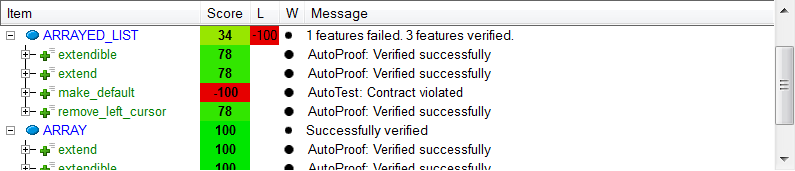
\includegraphics[width=\columnwidth]{images/va_screenshot.png}
\caption{Example report of \EVE, showing scores of classes and routines. The third column displays the lowest negative score among the routines of each class.}
\label{fig:motivating-screenshot}
\end{figure}

While Adam is busy fixing the error, testing cannot proceed on the same class. Even if the creation procedure were correct, routine \e{remove_left} would remain arduous for automated testing techniques because its precondition is relatively complex; a random-based approach to the generation of test cases requires specialized techniques and a long running time to select objects satisfying the clauses in lines~\ref{l:va:4}--\ref{l:va:5} \cite{WEI10}.
\EVE circumvents these limitations by running a static proof, which analyzes individual routines and does not need a correct creation procedure. The proof succeeds in establishing that the invocation of \e{remove} (line~\ref{l:va:3}) is correct and ensures the postcondition of \e{remove_left}: the routine is correct and no testing is needed (Figure~\ref{fig:motivating-screenshot}).


Later, as soon as the constructor of \e{ARRAYED_LIST} is fixed, \EVE continues its work and exhaustively tests the implementation of \e{is_equal} finding no postcondition violations. This is not as good as a correctness proof, but it comforts Adam's confidence in the reliability of \e{is_equal}, and it is the best result possible for a routine whose implementation can be analyzed only as black-box.

Although it only uses some of \EVE's features, this scenario illustrates how \EVE can help develop correct applications with little overhead over standard practices:
\begin{itemize}

\item
\EVE is completely automatic and integrated in a full-fledged IDE.

\item
It supports verification of functional correctness specifications embedded as contracts (pre and postconditions, class invariants, intermediate assertions).

\item
It transparently manages different verification engines to complement their strengths, supports the full programming language Eiffel, and provides fast feedback to users.

\item
It only displays such feedback when needed, to encourage focus on the most egregious errors, and to increase the users' confidence in the correctness of an implementation based on the available evidence.
\end{itemize}
%============================================================================
\section{The Tools of \EVE} \label{tools-of-eve}
%============================================================================

The integrated verification techniques currently available in \EVE 
and partially illustrated in the preceding example session relies on several 
tools that are integrated in \EVE: \AutoProof, \AutoTest, and the \Inspector, which are now presented.

%----------------------------------------------------------------------------
\subsubsection{\AutoTest}
%----------------------------------------------------------------------------

\AutoTest~\cite{MEYER09}---now a standard component of commercial EiffelStudio---is a fully automatic contract-based testing tool.
\AutoTest generates objects by random calls to creation procedures.
Preconditions select valid inputs and postconditions serve as oracles: every test case consists of the execution of a routine on objects satisfying its precondition; if executing the routine violate its postcondition or calls another routine without satisfying its precondition, the routine tested has a fault.
\AutoTest is fully automatic and does not need any user input. Since contracts are used as test oracles, the tool can find functional correctness bugs.
A failing test case provides a concrete error report which is useful for debugging.

Like any dynamic technique based on execution, \AutoTest handles every feature of the source language (Eiffel).
Among its limitations, instead, is that random testing can take several hours to find the most subtle faults, and that complex specifications can exacerbate this problem.


%----------------------------------------------------------------------------
\subsubsection{\AutoProof}
%----------------------------------------------------------------------------

\AutoProof is an auto-active verifier of full functional correctness and has been described in Chapter~\ref{sec:ap}.
\AutoProof supports some advanced language constructs such as function objects (agents in Eiffel terminology). Nonetheless, some features of Eiffel---most notably exceptions and floating point arithmetic---are still unsupported and routines using them are not adequately translated to Boogie.
The performance of \AutoProof depends on the quality of contracts available; accurate contracts improve the modularity of the analysis which can then also verify partial implementations.


%----------------------------------------------------------------------------
\subsubsection{\Inspector}
%----------------------------------------------------------------------------

The \Inspector~\cite{ZURFLUH14} is a light-weight code analysis tool to find code smells and simple coding errors along the lines of PMD for Java~\cite{PMD} or FxCop for C\#~\cite{FXCOP}. The \Inspector has an extendible rule system and a large set of implemented rules focusing on code smells like overly complex implementations or simplifiable expressions and also a few coding errors like wrongly used loop iterators. The analysis is in general quick and supports the full Eiffel language.



%============================================================================
\section{Advantages of Being Static and Dynamic}
%============================================================================

From a user's perspective, \EVE's integration of static and dynamic tools can make verification more effective and agile in a variety of scenarios.

\begin{itemize}

\item 
\emph{Modularity and scalability.}
Static verification is more modular and scales better to large systems made of several classes.
It can also verify routines of deferred (abstract) classes which cannot be tested because they cannot be instantiated.
This indirectly improves the performance of testing as well, because the testing effort can focus on routines or classes not proved correct.

Conversely, whenever testing uncovers a faulty routine, the static tool stops trying to verify that routine.
This policy may be broken down to individual clauses: for example, if testing finds a run of \e{remove_left} (Figure~\ref{tab:motivating-example}) violating the postcondition clause \e{count = old count - 1}, it may still be worthwhile to try to prove the other clause.

\item
\emph{Concrete counterexamples.}
Dynamic analysis provides concrete reports of errors, which make debugging easier. For example, the following trace documents the error in the creation procedure \e{make_default} of Figure~\ref{tab:motivating-example}:
\begin{erunning}
create {ARRAYED_LIST} l.make_default (1)
-- Inside $\textit{make\_default}$:
l_v := Void ; Precursor (1) ; extend (l_v) -- $l\_v$ is $\mathbf{Void}$
\end{erunning}

\item 
\emph{Partial implementations.}
Classes that have a faulty creation procedure or are deferred cannot be instantiated; testing cannot proceed in this case unless the constructor is fixed or an implementation of every routine is available.
Static techniques do not incur these limitations: as illustrated in the example of Section~\ref{sec:va:example}, they can verify individual implemented routines even if others in the same class are deferred.

\item
\emph{Black-box verification.}
Many core libraries rely on routines implemented through calls to low-level external routines (typically, in the Eiffel case, C functions); an example was \e{is_equal} in Figure~\ref{tab:motivating-example}.
Such routines are inaccessible to static analysis but are still testable. The integrated results of static and dynamic analysis on classes with such external routines reinforce the confidence in the correctness of the overall system.

\item
\emph{Abstract vs.~runtime behavior.}
Combining static and dynamic analysis can help detect discrepancies between the runtime behavior of a program and its idealized model.
Examples are overflows and out-of-memory errors, which are often not accounted for in an abstract specification assuming perfect arithmetic and infinite memory.
Consider, for example, a routine that updates the balance of a bank account as a result of a deposit operation:
\begin{erunning}
deposit (amount: INTEGER)
	require amount > 0
	do balance := balance + amount
	ensure balance > old balance
	end
\end{erunning}
\AutoProof with default options models the type \e{INTEGER} as mathematical integers and verifies that the routine is correct (an option exist to enable overflow checks).
\AutoTest, however, can still find a bug which occurs when \e{old balance + amount} is greater than the largest integer value representable and \e{balance} overflows.
It is then a matter of general policy whether one should change the postcondition or the implementation.
In any case, the comparison of the results of static and dynamic analysis clearly highlights the problem and facilitates the design of the best solution.

\item
\emph{Complex contracts.}
Complex contracts considerably slow down automatic testing, both because their runtime evaluation incurs a significant overhead and because random generation takes a long time to build objects that satisfy complex preconditions.
Contracts may even in some cases be non-executable because they involve predicates over infinite sets or ghost code; for example, the invariant of a class modeling a hash function requires that the hash code of every possible object (an infinite set) be a non-negative integer.
Static techniques can help in all such scenarios: it may be easier to prove the correctness of a routine if the precondition is complex, and hence also stronger; complex postconditions boost modular verification.
\end{itemize}


These observations highlight the usefulness of treating proofs and tests as complementary and convergent techniques.
There is indeed no contradiction; in particular, with the purpose of tests being entirely defined as attempting to make programs fail~\cite{MEYER08}, a useful (that is, failed) test is a proof that the program is not correct. The approach illustrated by \EVE is then to combine tools that can prove a program correct (such as \AutoProof) and tools that can prove a program incorrect (\AutoTest); as soon as a user has written a new program element, the two will start in the background, each with its own specific goal, prove or disprove; in favorable situations, one of them will reach its goal fast, providing the user with a fast response of correctness or incorrectness.



%============================================================================
\section{The Design of an Integrated Verification Environment}\label{sec:va:general-mechanisms}
%============================================================================

The \EVE integrated verification environment is built on top of the EiffelStudio IDE and supplements it with functionalities for verification.

%----------------------------------------------------------------------------
\subsection{Contracts}
%----------------------------------------------------------------------------

The choice of Eiffel as programming language ensures that we rely on formal specification elements embedded in the program text as \emph{contracts} (pre and postconditions, class invariants, and other annotations).
Since correctness is a relative notion (being dependent on a specification), every verification activity requires \emph{some form} of specification.
Empirical evidence suggests that formal specifications in the form of contracts are a good compromise between the rigor required by formal techniques and the kind of effort that practitioners are able, or willing, to provide \cite{CHALIN06,POLIKARPOVA09}.

Not all contracts must be written by programmers: the architecture of \EVE can accommodate components for \emph{specification inference} to help users write better and stronger contracts.
This particular property, however, is not emphasized in the present discussion, which focuses on the integration of static and dynamic analysis assuming some contracts are available.

%----------------------------------------------------------------------------
\subsection{Automation}
%----------------------------------------------------------------------------

A defining characteristic of the tools in \EVE is that they are automatic and can do most of the work without any explicit input from the user, assuming the presence of contracts which Eiffel  programmers are already used to provide.
In order to decouple the machinery of the individual verification tools and to filter out their output, \EVE relies on a blackboard architecture~\cite{HUNT02} shown in Figure~\ref{fig:blackboard}.

\begin{figure}[!ht]%
\centering
\includegraphics[width=0.8\columnwidth,page=4]{images/drawings.pdf}
\caption{\EVE's blackboard architecture (gray boxes currently not implemented).}%
\label{fig:blackboard}%
\end{figure}


A \emph{controller} is responsible for triggering the various tools when appropriate, invisibly to the users. 
The controller bases its decisions on what the user is currently doing, which resources are available, and the results of previous verification attempts.
The latter are collected in a \emph{data pool} where every verification tool stores the results of its runs.
Users do not directly read the output of individual tools in the data pool.
Instead, the controller summarizes the output data and displays individual tool results only upon explicit user request.

A major design decision of \EVE was to make the verification mechanisms as unobtrusive as possible.
Users can continue using the IDE and their preferred software development process as before; the verification techniques are an additional benefit, available on demand and compatible with the rest of the IDE's tools.
In the same way that type checking adds a new level of help on top of the more elementary mechanisms of syntax error checking, \EVE provides reports from proofs and tests on top of the simple verification techniques provided by type checking.

%----------------------------------------------------------------------------
\subsection{Interaction with the user}
%----------------------------------------------------------------------------

Users have currently two ways to control the verification: (1) manually launch the tools or (2) use the fully automatic controller.
When using manual mode, the user chooses which tool to run on a specific class.
The tool will run in the background and the result will be added to the data pool when available, which will also automatically update the summary display.
Automatic mode has only the limited option of being enabled or disabled.
Even when enabled, verification never interferes with the more traditional development activities: \EVE works in the background on the latest compiled version of the system, and displays a summary of the verification results through an interface similar to that used to signal syntax or type errors in standard IDEs (Figure~\ref{fig:motivating-screenshot}).
At any time, the user can browse through the \emph{result list}, which links back to the parts of the program relevant for each message, and decide to revise parts of the implementation or specification according to the suggestions provided by \EVE.

Every entry in the result list has a \emph{score}: a quantitative estimate of the correctness or incorrectness of the associated entry, based on the evidence gathered so far by running the various tools.
The score varies over the real interval $[-1,1]$ (In the user interface the scale is, for more readability, $-100$ to $+100$, with rounding to the closest integer). 
A positive score indicates that the evidence in favor of correctness prevails, whereas a negative score characterizes evidence against correctness. The absolute value of the score indicates the level confidence: $1$ is conclusive evidence of correctness (for example a successful correctness proof), $-1$ is conclusive evidence of incorrectness (for example a failing test case), and $0$ denotes lack of evidence either way. Figure~\ref{fig:motivating-screenshot} shows an example of report with scores and stripes colored accordingly. Section~\ref{sec:va:scores} discusses how the score is computed for the verification tools currently integrated in \EVE.


%----------------------------------------------------------------------------
\subsection{Modularity and granularity}
%----------------------------------------------------------------------------

Object-oriented design emphasizes modularity, from which verification can also benefit.
While the level of granularity achievable by an integrated verification environment ultimately depends on the level of granularity provided by the tools it integrates, \EVE orients verification at the two basic levels of encapsulation provided by the object-oriented model: \emph{classes} and \emph{routines} within a class.
\EVE associates \emph{correctness scores} with items at both levels. Additional information may be attached to a correctness score, such as the line where a contract violation occurs in a test run, or the abstract domain used in an abstract interpretation analysis.
For large systems, it is also useful to have scores for highest levels of abstraction, such as groups of classes or entire libraries, but in the present discussion we limit ourselves to routine and class levels.

The scores from multiple sources of data at the same level are combined with weighted averages, and define the correctness scores at coarser levels.  
For example, every tool $t$ tries to verify a routine $r$ in class $C$ and reports a correctness score $s_r^C(t) \in [-1,1]$.
The cumulative score for the routine $r$ is then computed as the normalized weighted average:
\begin{equation}
s_r^C \ =\ \frac{1}{\sum_{t \in T} w_r^C(t)} \cdot \sum_{t \in T} w_r^C(t)s_r^C(t)
\label{eq:routine}
\end{equation}
where $w_r^C(t) \in \mathbb{R}_{\geq 0}$ denotes the weight (or \emph{confidence}) of the tool $t$ on routine $r$.
A similar expression computes the cumulative score $s^C$ for a class $C$ from the scores $s_r^C$ of its routines and their weights $w_r^C$:
\begin{equation}
s^C \ =\ \frac{1}{\sum_{r \in R} w_r^C} \cdot \sum_{r \in R} w_r^Cs_r^C
\label{eq:class}
\end{equation}

The weights take various peculiarities into account:
\begin{itemize}
\item
A tool may not be able to handle certain constructs: its confidence should be scaled accordingly.
For example, a tool unable to handle exceptions appropriately has its score reduced whenever it analyzes a routine which may raise exceptions.

\item
The results of a tool may be critical for the correctness of a certain routine.
For example, a quality standard may require that every public routine be tested for at least one hour without hitting a bug; correspondingly, the weight $w_r^C(t)$ for public routines $r$ would be high for testing tools and low (possibly even zero) for every other tool.

\item
The correctness of a routine may be critical for a class; then the routine score should have a higher weight in determining the class cumulative score.

\item
More generally, the weight may reflect suitable \emph{metrics} that estimate the criticality of a routine according to factors such as the complexity of its implementation or specification, whether it is part of the interface of public, and the number of references to it in clients or within the containing class.

\item
Similar metrics are applicable at other levels of granularity, for example to weigh the criticality of a class within the system.

\end{itemize}

\EVE provides default values for all the weights (Section~\ref{sec:va:scores}), but users can override them to take relevant domain knowledge into account.





%----------------------------------------------------------------------------
\subsection{Extensibility}
%----------------------------------------------------------------------------

The architecture of \EVE is \emph{extensible} to include more tools of heterogeneous nature.
The user interface will stay the same, with the blackboard controller being responsible for managing the tools optimally and only reporting the results through the summary scores described above.

The architecture can also accommodate tools that, while not targeted to verification in a strict sense, enhance the user experience.
For example, tools for assertion inference---such as AutoInfer \cite{WEI11} developed by other members of my group---can complement user-provided contracts and improve the performance of approaches that depend on contracts.
The controller can activate assertion inference when the verification machinery performs poorly and when metrics suggest that the code is lacking sufficient specifications.
The assertion inference tools themselves may sometimes re-use the results of other tools; for example AutoInfer relies on the test cases generated by \AutoTest.
Finally, \EVE can show the inferred assertions in the form of suggestions, in connection with the results of other verification activities.
For example, it could display an inferred loop invariant with the report of a failed proof attempt, and suggest that the invariant can make the correctness proof succeed if added to the specification.
The current implementation of \EVE does not integrate such suggestions mechanisms yet. %, but the architecture is designed with these extensions in mind.



%============================================================================
\section{Correctness Scores for \EVE}\label{sec:va:scores}
%============================================================================

Equation~\ref{eq:routine} on page~\pageref{eq:routine} gives the correctness score for a routine $r$ of class $C$; now, consider a set of tools $T =\{p, t, e\}$, where $p$ denotes \AutoProof, $t$ denotes \AutoTest, and $e$ denotes \Inspector.



\subsection{General principles for scores}

We noted earlier that an interesting test, that is to say a failed test, is a proof of incorrectness. This is of course another form of Dijkstra's famous observation about testing---but restated as an argument \emph{for} tests rather than a criticism of the notion of testing. 
This observation has two direct consequences on the principles for computing correctness scores.

First, it is relatively straightforward to assign scores to the result of a testing tool when it reports errors: assign a score of $-1$, denoting certain incorrectness, to every routine where testing found an error.
In certain special circumstances, the score might be differentiated according to the severity of the fault; for example a bug that occurs only if the program runs for several hours may be less critical than one that occurs earlier, if the system is such that it is reset every 45 minutes.
In most circumstances, however, it is better to include such domain information in the specification itself and to treat every reported fault as a routine error.
Then, different routines may still receive a different weight in the computation of the score of a class (Equation~\ref{eq:class} on page~\pageref{eq:class})---for example, a higher weight to public routines with many clients.

The second consequence is that it is harder to assign a positive score sensibly to routines passing tests without errors.
It is customary to assume that many successful tests increase the confidence of correctness; hence, this could determine a positive correctness score, which increases with the number of tests passed, the diversity of input values selected, or the coverage achieved according to some coverage
criteria such as branch or instruction coverage.
In any case, the positive score should be normalized so that it never exceeds an upper limit strictly less than $1$, which denotes certain correctness
and is hence unattainable by testing.

For verification tools that are sound, a successful proof should generally give a score of $1$.
Certain aspects of the runtime behavior, such as arithmetic and memory overflows as discussed above, may still leak in some unsoundness if the static verifier does not model them explicitly; in such cases the score for a successful proof may be scaled down in routines with a specification that depends on such aspects.

Which score to assign to a static verifier reporting a failed proof attempt depends on the technique's associated guarantee of \emph{completeness}.
For a complete tool, a failed proof denotes a certain fault, hence a score of $-1$.
If the tool is incomplete, a failed proof simply means ``I don't know''; whether and how this should affect the score depends on the details of the technique.
For example, partial proofs may still increase the evidence for correctness and yield a positive score.


\subsection{Score and weight for \AutoTest}

If \AutoTest reports a fault in a routine $r$ of class $C$, the correctness score $s_r^C(t)$ becomes $-1$.  This score receives a high weight $w_r^C(t) = 100$ by default; the user can adjust this value to reflect specific knowledge about the criticality of certain routines over others with respect to testing.

When \AutoTest tests a routine $r$ of class $C$ without uncovering any fault, the score $s_r^C(t)$ increases proportionally to the length of
the testing session and the number of test cases executed, but with an upper limit of $0.9$.
With the default settings, this maximum is reached after 24 hours of testing and $10^4$ test cases executed without revealing any error in $r$.
Users can change these parameters; the default settings try to reflect the specificities of random testing shown in repeated experiments~\cite{WEI12}. 
We decided against using specific coverage criteria such as branch coverage in the calculation of the routine score, as the experiments suggest that for example the correlation between branch coverage and the number of uncovered faults is weak.



\subsection{Score and weight for \AutoProof}

\AutoProof implements a sound but incomplete proof technique.
The score $s_r^C(p)$ for a routine $r$ of class $C$ is set accordingly:
\begin{itemize}
	\item 
     a successful proof yields a score of $1$;
	\item
     an out-of-memory error or a timeout are inconclusive and yield a $0$;
	\item
     a failed proof with abstract trace may be a faint indication of
     incorrectness: the abstract trace may not correspond to any
     concrete trace (showing an actual fault), but it often suggests
     that a proof might be possible with more accurate assertions.
     The score is then $-0.3$ to reflect this heuristic
     observation.
\end{itemize}

The weight $w_r^C(p)$ takes into account the few language features that are currently unsupported: if $r$'s body contains a feature that is not supported (e.g. exceptions), $w_r^C(p)$ is conservatively set to zero, if $r$'s body contains a feature that is partially supported (e.g. floating point arithmetic), $w_r^C(p)$ is set to a value between $0$ and $1$.
In all other cases, $w_r^C(p)$ is $1$ by default.


\subsection{Score and weight for \Inspector}

The \Inspector, unlike \AutoTest and \AutoProof, does not focus on functional correctness. It has only very few rules that reveal a definite coding error and most of the rules indicate bad code quality or even just adherence to coding guidelines.
While rule violations in general indicate bad code quality they lend only little evidence for incorrectness and the absence of rule violations has no value for correctness at all.
We account for that by setting the score $s_r^C(e)$ and weight $w_r^C(e)$ accordingly.

The score given by \Inspector reflects the kind of rules violated. Each rule is categorized as either a \emph{hint}, a \emph{warning} or an \emph{error}. We ignore the hint category entirely, as this is only indicative of coding style. If \Inspector finds a violation of an error rule the score is set to $-1$ and if only warning rules are violated we give a negative score up to a maximum of $-0.3$ depending on the number of rule violations to reflect the intuition that complex code has a higher probability of errors. The increase to the negative score is linear in the number of rule violations found and capped at the maximum value of $-0.3$.

The weight also depends on the type of the violated rules.
We set the weight to $100$ if one of the few error rules is violated, similar to the case where \AutoTest finds an error in the program.
When only warning rules are violated we set the weight to $1$ and when no rules are violated the weight becomes $0$.
Therefore, the \Inspector does not contribute to the overall score if it does not find any rule violations.

\subsection{Routine weights}

Equation~\ref{eq:class} (page~\pageref{eq:class}) combines the scores $s_r^C$ of every routine $r$ of class $C$ with weights $w_r^C$ to determine the cumulative score of $C$.
The weights $w_r^C$ should quantify the relevance of routine $r$ for the correctness of class $C$.
Different metrics could be used to automatically infer the importance of a routine:
\begin{itemize}
\item
Routines usable by other classes might have a higher impact on the perceived correctness of a class.

\item
Routines with higher complexity can be considered more important. A high complexity indicates that the routine is performing an important operation, therefore its correctness should be more important for the correctness of the class.

\item
Faults in a routine with many clients have potentially higher impact. When a routine has many clients, its importance could be increased accordingly.

\item
Using run-time profiling information, the relative time spent executing a routine or the relative number of calls to a routine could be used to weigh the importance of routines. The higher such numbers---execution time or calls to a routine---the higher the importance of a routine.

\end{itemize}

Despite the possibility to infer the routine importance automatically, it is the developer who has a better understanding of the overall system design and can decide best which routines are more important.

\EVE supports a simple way give developers control over the importance setting of routines: every routine has an optional \emph{importance} flag which takes the values \emph{low}, \emph{normal} (the default), and \emph{high}.
$w_r^C$ is then $$w_r^C \ =\ v_r^C \cdot i_r^C$$
The visibility of $r$ determines $v_r^C$, which is $2$ if $r$ is public and $1$ otherwise.
The importance of $r$ determines $i_r^C$, which is $2$ if $r$ has high importance, $1$ if it has normal importance, and $1/2$ if it has low importance.



%============================================================================
\section{Usage Scenarios}
%============================================================================


How serviceable is \EVE's score which combines the results of different verification tools, as opposed to considering the tools' outputs individually?
This section outlines a few straightforward scenarios that compare the output given by \AutoProof or \AutoTest in isolation against \EVE's combined output; they show the greater confidence supplied by \EVE, and the straightforward interpretability of its output.
%
The example models attributes of an individual with a class \e{PERSON}. Table~\ref{table:person_results} lists 8 routines of the class to be verified; for each routine, the table reports the score and weight of \AutoProof and \AutoTest within \EVE, and the corresponding combined score.

\begin{table}[!htb]
\centering
\scriptsize
\begin{tabular}{l l l r r}

  \textbf{Item} & \textbf{Tool} & \textbf{Result} & \ \textbf{Weight} & \ \textbf{Score} \\ \hline
  
  \e{set_age}
     & \AutoProof & Verified successfully & 1.0 & 1.00 \\
     & \AutoTest & No errors found & 1.0 & 0.90 \\
     & \Inspector & No violations found & 0.0 & 0.00 \\
     &  \textbf{Routine score} & & & \textbf{0.95} \\ \hline
  \e{set_weight}
     & \AutoProof & Verified successfully & 1.0 & 1.00 \\
     & \AutoTest & No errors found & 1.0 & 0.90 \\
     & \Inspector & No violations found & 0.0 & 0.00 \\
     &  \textbf{Routine score} & & & \textbf{0.95} \\ \hline
  \e{set_height}
     & \AutoProof & Postcondition violation & 1.0 & -0.30 \\
     & \AutoTest & Postcondition violation & 100.0 & -1.00 \\
     & \Inspector & Error: self-assignment & 100.0 & -1.00 \\
     &  \textbf{Routine score} & & & \textbf{-1.00} \\ \hline
  \e{set_name}
     & \AutoProof & Proof failed & 0.5 & -0.30 \\
     & \AutoTest & No errors found & 1.0 & 0.90 \\
     & \Inspector & No violations found & 0.0 & 0.00 \\
     &  \textbf{Routine score} & & & \textbf{0.50} \\ \hline
  \e{increase_age}
     & \AutoProof & Verified successfully & 0.5 & 1.00 \\
     & \AutoTest & Overflow detected & 100.0 & -1.00 \\
     & \Inspector & No violations found & 0.0 & 0.00 \\
     &  \textbf{Routine score} & & & \textbf{-0.99} \\ \hline
  \e{age_difference}
     & \AutoProof & Verified successfully & 0.5 & 1.00 \\
     & \AutoTest & No errors found & 1.0 & 0.90 \\
     & \Inspector & Warning: local not read & 1.0 & -0.10 \\
     &  \textbf{Routine score} & & & \textbf{0.60} \\ \hline
  \e{print_id_card}
     & \AutoProof & Inapplicable & 0.0 & 0.00 \\
     & \AutoTest & No errors found & 1.0 & 0.90 \\
     & \Inspector & No violations found & 0.0 & 0.00 \\
     &  \textbf{Routine score} & & & \textbf{0.90} \\ \hline
  \e{apply_command}
     & \AutoProof & Verified successfully & 1.0 & 1.00 \\
     & \AutoTest & Inapplicable & 0.0 & 0.00 \\
     & \Inspector & No violations found & 0.0 & 0.00 \\
     &  \textbf{Routine score} & & & \textbf{1.00} \\ \hline
  \e{PERSON}
     & \textbf{Class score} & & & \textbf{0.41} \\ \hline
     \\
\end{tabular}
\caption{Individual and combined results for class \e{PERSON}.}
\label{table:person_results}
\end{table}

Routines \e{set_age} and \e{set_weight} demonstrate a favorable scenario, where \AutoProof and \AutoTest can provide strong positive evidence indicating correctness and \Inspector finds no rule violations. The overall score is, correspondingly, quite high, but it still falls short of the maximum because testing can never prove the absence of errors with 100\% confidence. 

Routine \e{set_height} shows the opposite scenario, where all three tools report a failure. The routine has an incorrect implementation which triggers one of the few \emph{error} rules of \Inspector. \AutoProof and \AutoTest both report a postcondition violation.
The two tools \AutoTest and \Inspector have very high confidence when they find errors, thus they both use a very high weight.

Routine \e{set_name} relies on the object comparison semantics, which \AutoProof overapproximates. 
In this case, a failed proof does not necessarily indicate an error in the routine, hence it only accounts for a mildly negative score.
When \AutoTest does not find any error after thorough testing, the combined score becomes visibly positive, while still leaving a margin of uncertainty given the lack of conclusive evidence either way.

Routine \e{increase_age} includes integer arithmetic, which might produce overflow. 
\AutoProof can verify the routine, but \EVE is aware that overflow checking is disabled and the proof scheme models integers as mathematical integers, hence it weights down the value of the successful proof because the abstraction may overlook overflow errors.
Indeed, \AutoTest reveals an overflow when executing the routine with the maximum integer value. 
The combined score indicates that there is an error, which \AutoTest discovered beyond the limitations of \AutoProof. 
Another routine \e{age_difference} also uses integer arithmetic but it is correct.
\EVE still scales down \AutoProof's score accordingly; in this case, however, \AutoTest does not find any error, hence the overall score grows high: the uncertainties of the two tools compensate each other and the cumulative score indicates confidence.
Additionally, \Inspector reports a warning for this routine due to some leftover debugging code which slightly reduces the overall score of the routine.

Routines \e{print_id_card} and \e{apply_command} demonstrate how \EVE's combination of tools expands the applicability of verification: \e{print_id_card} uses string manipulations and console output, unsupported by \AutoProof, whereas \e{apply_command} uses agents, unsupported by \AutoTest. \EVE relies entirely on the only applicable tool in each case.


The overall class score (last line of Table~\ref{table:person_results}) uses a uniform weight for the routines; the score concisely indicates that considerable effort has been successfully invested in the class's verification, but some non-trivial issues are open. 

%############################################################################
\section{Related Work}
\label{sec:va-related}
%############################################################################



A few authoritative researchers have pointed out the potential of combining static and dynamic techniques~\cite{RAJAMANI09,ERNST10,FRASER10} to make verification more usable.

Some of the aforementioned testing tools~\cite{GODEFROID05,SEN05,CADAR08} already leverage lightweight static analyses to boost the performance of automated testing. 
Pex~\cite{TILLMANN08} is another scalable automatic testing framework, which relies more heavily on static methods: it exploits a variant of dynamic symbolic execution where an automated theorem prover (Z3) analyzes the symbolic executions to improve code coverage.  Pex uses parameterized unit tests~\cite{TILLMANN05} as specifications. 
This makes it possible to test fairly sophisticated properties, but it also requires users to produce specifications in this customized form; contract specifications, however, seem more palatable to practitioners~\cite{CHALIN06b}.

DASH~\cite{RAJAMANI09} combines static and dynamic verification with an approach extending the software model-checking paradigm~\cite{BEYER07}: DASH's algorithm to generate exhaustive tests maintains a sound abstraction of the program, which can be used to construct automatically a correctness argument.

The few recent attempts at combining static and dynamic techniques tend to be specific conservative extensions of basic methods; the approach described here tries integration at a higher level to avail the complementarity of static and dynamic techniques to a larger extent.

The SPARK Pro IDE~\cite{SPARKPRO} provides analysis and verification tools for the SPARK programming language~\cite{BARNES03}. The tools are integrated in the user interface and provide feedback through errors and warnings for different types of analyses and---given contract equipped program---verify the functional correctness of the program.

Frama-C~\cite{CUOQ12,CORRENSON12} is a tool-set to statically analyze C code. In addition to providing a plug-in based system for different types of analyses, Frama-C can be used to verify properties expressed in the ACSL specification language~\cite{ACSL}.

SIDE~\cite{LOGOZZO12b}, a Semantic IDE, leverages the CodeContracts checker~\cite{FAEHNDRICH10} to analyze programs in real time. The analysis can be used to verify absences of runtime errors, suggest fixes for errors, and infer contracts in the form of pre- and postconditions.



\imagechapter
%############################################################################
\chapter{\AutoProof: a Tool for Auto-active Verification}
\label{sec:ap}
\chapterimage{images/autoproof}
%############################################################################


This chapter describes \AutoProof, our auto-active verifier for functional properties of object-oriented programs.
In its latest development state, \AutoProof offers a unique combination of features that make it a powerful tool in its category and a significant contribution to the state of the art.
\AutoProof targets a real complex object-oriented programming language (Eiffel)---as opposed to more abstract languages designed specifically for verification.
It supports most language constructs, as well as a full-fledged verification methodology for heap-manipulating programs based on a flexible annotation protocol, sufficient to completely verify a variety of programs and verification challenges that are representative of object-oriented idioms as used in practice (see Chapter~\ref{sec:method}).
\AutoProof was developed with usability and extensibility in mind: it features techniques to help debug failed verification attempts so as to offer an incremental user experience, its annotation library can be augmented with new abstract models, and its implementation can be easily adapted to accommodate changes in the input language.


%############################################################################
\section{Introduction}
\label{sec:ap-intro}
%############################################################################


\AutoProof is an auto-active verifier of functional correctness working on Eiffel programs and using Boogie~\cite{LEINO08} as a back-end verifier. Figure~\ref{fig:ap-workflow} shows the general workflow of using \AutoProof. It takes compiled Eiffel programs annotated with contracts and translates them to Boogie code. The Boogie verifier is then invoked on the generated Boogie code transforming the intermediate Boogie program to verification conditions. These verification conditions are finally checked by an SMT solver (currently Z3). The result of the verification is then traced back to Eiffel code and displayed to the user.

\begin{figure}[!htb]
\centering
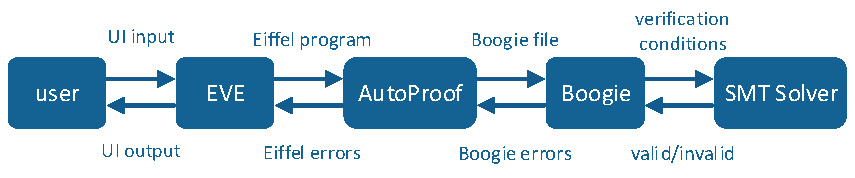
\includegraphics[width=\columnwidth,page=1]{images/drawings.pdf}
\caption{High-level overview of the \AutoProof verification workflow.}
\label{fig:ap-workflow}
\end{figure}

\AutoProof does modular verification on the level of routines. Each routine is checked separately and for calls inside a routine only the callee's specification is used. This allows to verify Eiffel systems piece by piece, and, when a routine body is changed, only the changed routine must be reverified. \AutoProof is available online as well as integrated in \EVE, the Eiffel Verification Environment IDE~\cite{EVE}.


%############################################################################
\section{User Interface}
\label{sec:ap-interface}
%############################################################################

\AutoProof is available in two modes of operation: (1) through a graphical interface integrated in the \EVE IDE and (2) as a command-line tool. In addition, there are two different web interfaces that gives access to the command-line version of \AutoProof, each with different limitations.


%============================================================================
\subsection{\AutoProof in \EVE}
%============================================================================

\EVE is the Eiffel Verification Environment, an Eiffel IDE based on EiffelStudio~\cite{EIFFELSTUDIO}. \EVE contains various research tools including \AutoProof. In \EVE, \AutoProof is available as a separate tool panel. Figure~\ref{fig:eve-tool-panel} shows EVE with the \AutoProof panel open in the bottom left. 

\begin{figure}[ht]
\centering
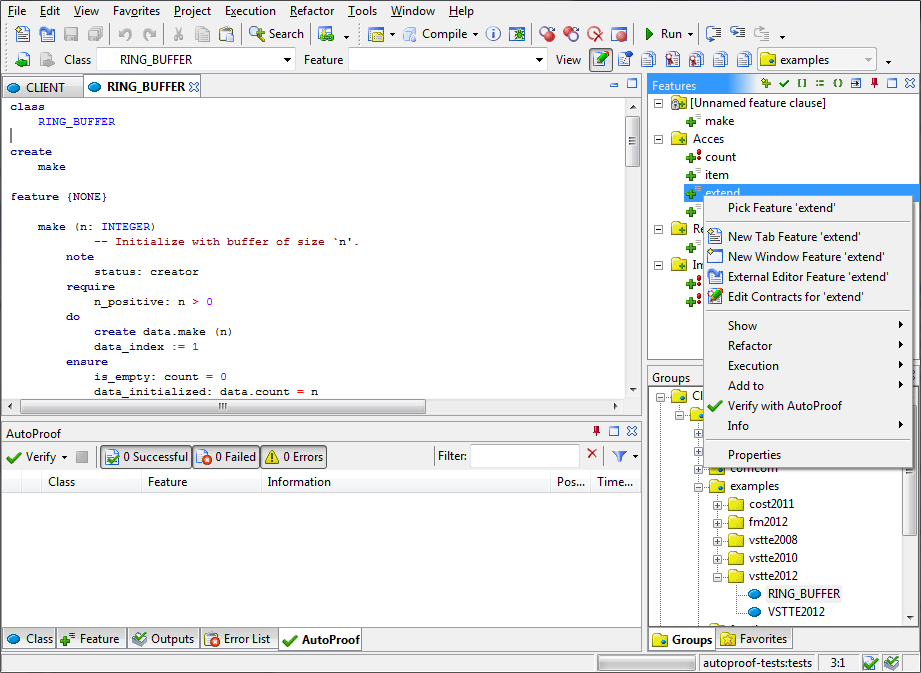
\includegraphics[width=\textwidth]{images/eve_layout_with_context_menu.png}
\caption{The \AutoProof tool panel in \EVE (lower left) and the context menu of a feature (right side).}
\label{fig:eve-tool-panel}
\end{figure}

%----------------------------------------------------------------------------
\subsubsection{Running \AutoProof}
%----------------------------------------------------------------------------

The scope of the input to \AutoProof can be selected by interacting with the \emph{Verify} button:
\begin{itemize}
\item \emph{Verifying a single feature}: pick-and-drop a feature on the button.
\item \emph{Verifying a single class}: either open a class in the editor and click the button or pick-and-drop a class on the button.
\item \emph{Verifying all classes in a cluster or library}: either open a cluster in the editor and click the button, pick-and-drop a cluster or library on the button, or use the drop-down arrow on the button to verify the cluster the currently selected class is in.
\item \emph{Verifying the whole system (excluding libraries)}: use the drop-down arrow on the button and select \emph{Verify System}
\end{itemize}

The user can also right-click any feature, class, cluster, or library and select the \emph{Verify with \AutoProof} option from the context menu (see right side of Figure~\ref{fig:eve-tool-panel}).

\AutoProof will always check that the system compiles successfully with the Eiffel compiler before starting the verification. This ensures that the code that is verified is valid Eiffel code. Only one instance of \AutoProof can run at the same time, so during the execution of \AutoProof the \emph{Verify} button is disabled while the red \emph{stop} button next to it is enabled. With the stop button the user can abort a long-running verification if necessary.



%----------------------------------------------------------------------------
\subsubsection{Displaying results}
%----------------------------------------------------------------------------

\begin{figure}
\centering
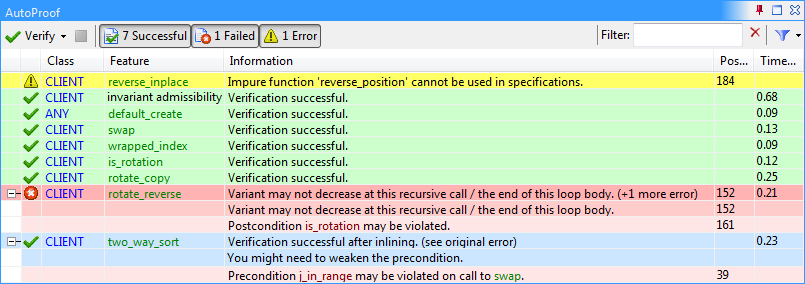
\includegraphics[width=\columnwidth]{images/eve_panel_results.png}
\caption{The \AutoProof panel showing the results of a verification.}
\label{fig:eve-tool-result}
\end{figure}

After the verification is finished, \AutoProof displays the results of the verification in the tool panel. It displays the verification result for each individual routine separately. Figure~\ref{fig:eve-tool-result} shows an example of running \AutoProof. There are four possible outcomes per routine:
\begin{itemize}
\item \colorbox[HTML]{CCFFCC}{Green row:} The verification was successful.
\item \colorbox[HTML]{FFBBBB}{Red row:} The verification failed. An error message will indicate what type of assertion was not verified correctly and, if possible, indicate the assertion tag and line number of the assertion. It is also possible that there are multiple violations for a single routine in which case the row can be expanded to show all messages.
\item \colorbox[HTML]{FFFF66}{Yellow row:} There was invalid input to \AutoProof and the verification of that routine was not possible. This usually means an Eiffel construct is present that \AutoProof does not support or an Eiffel assertion is invalid in another way (e.g. an impure function is used in a contract).
\item \colorbox[HTML]{DDEEFF}{Blue row:} The verification was successful in the second step of two-step verification. The row can be expanded to show a possible suggestion of what the user can do to fix the original problem as well as the message of the failed first verification step.
\end{itemize}

In addition to the information about the routine and the message, the row will also indicate how long it took Boogie to verify that particular routine. The Eiffel elements such as class and feature names and the line number (if available) can be used to jump to the respective source location.

%----------------------------------------------------------------------------
\subsubsection{Verification options}
%----------------------------------------------------------------------------

The user can change the behavior of \AutoProof by enabling or disabling the following options:

\begin{itemize}
\item \emph{Two-step verification}: if enabled, a second verification attempt will be made on failed verifications.
\item \emph{Automatic inlining of routines}: if enabled, routines without postconditions will be automatically inlined.
\item \emph{Automatic loop unrolling}: if enabled, loops without a loop invariant will be automatically unrolled.
\item \emph{Generate postcondition predicates}: If enabled, \AutoProof will generate postcondition predicates and corresponding axioms to verify polymorphic calls.
\item \emph{Overflow checks}: if enabled, \AutoProof will check arithmetic operations for overflows.
\item \emph{Generate triggers}: if enabled, \AutoProof will generate triggers for quantified arithmetic expressions in Boogie.
\item \emph{Bulk or forked verification}: the user can choose between verifying all routines in one Boogie execution or running Boogie on each routine individually.
\end{itemize}


%============================================================================
\subsection{\AutoProof on the Command-line}
%============================================================================

Using \AutoProof on the command-line is similar to using the regular Eiffel compiler. In addition to specifying the Eiffel project, the user has to specify the \emph{-autoproof} option to launch \AutoProof after the Eiffel compilation succeeded. To set options of \AutoProof such as enabling or disabling arithmetic overflow checks, the user can add additional command-line flags for \AutoProof (see Appendix~\ref{manual:options} for details). Lastly, the user can also specify which classes and routines should be verified. If no selection is given, the whole system (excluding libraries) will be verified. The following command shows an example of launching \AutoProof with the project file \e{lcp.ecf} and overflow checking enabled on the single routine \e{LCP.client}:

\begin{lstlisting}[language=bash]
ec.exe -config lcp.ecf -autoproof -overflow LCP.client
\end{lstlisting}

The output of the verification will be printed to the console analogous to the graphical version of \AutoProof.


%============================================================================
\subsection{\AutoProof on the Web}\label{sec:ap:webui}
%============================================================================

There are two web-interfaces available for \AutoProof: (1) Comcom~\cite{APCOMCOM} and (2) E4Pubs~\cite{APE4PUBS}. Both of them can be used to deploy examples, provide an online editor to change the examples, and can run \AutoProof on the examples using the command-line interface of \AutoProof. There are different limitations and use cases though.

%----------------------------------------------------------------------------
\subsubsection{Comcom}
%----------------------------------------------------------------------------

\begin{figure}[p]
\centering
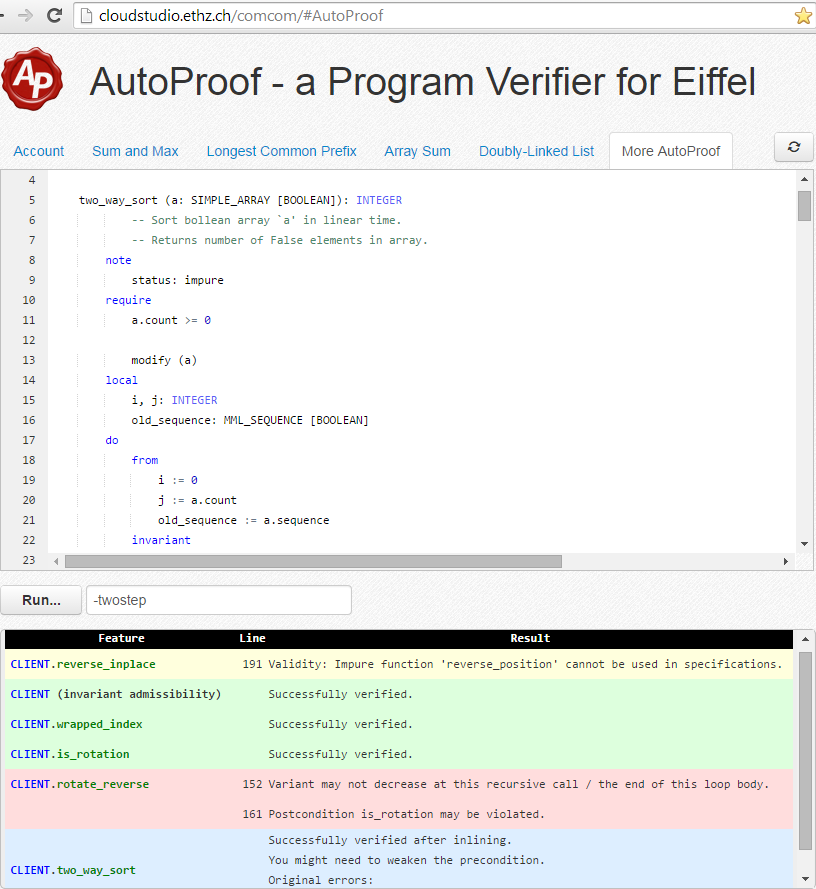
\includegraphics[width=\columnwidth]{images/comcom_screenshot.png}
\caption{Screenshot of comcom after running an example.}
\label{fig:ap-comcom}
\end{figure}

\emph{Comcom} is a web-interface for command-line tools. It features a list of predefined examples that the user can choose and modify as well as the possibility to write custom code from scratch and provide command-line arguments to \AutoProof. 
Figure~\ref{fig:ap-comcom} shows the interface of Comcom after running an example verification.

The limitation of \AutoProof on Comcom is the use of single-file examples. Since Eiffel only allows one class per file, the examples on Comcom have to be self-contained in one class. The user can use any class from the Eiffel base library, so it is still possible to write interesting examples and algorithms.

Due to Comcom's integration with the \emph{rise4fun} API, \AutoProof is also available on the rise4fun website~\cite{APRISE4FUN}.

%----------------------------------------------------------------------------
\subsubsection{E4Pubs}
%----------------------------------------------------------------------------

The second web-interface to \AutoProof is \emph{E4Pubs}, which stands for \emph{Eiffel 4 Publications}. It offers to host a predefined set of examples that can be verified with \AutoProof. Each example can---in contrast to---contain multiple classes. On the other hand, there is no possibility to write a custom example from scratch or provide command-line arguments. This web-interface is used to host examples for publications or to showcase features of \AutoProof, as each example has a unique URL and the examples can also be embedded in other websites. We use E4Pubs for example to create an interactive tutorial for \AutoProof~\cite{APTUTORIAL} and showcase benchmark examples~\cite{APREPO}.




%############################################################################
\section{Input Language Support}
\label{sec:ap-coverage}
%############################################################################


\AutoProof supports most of the Eiffel language as used in practice, obviously including Eiffel's native notation for contracts (specification elements) such as pre- and postconditions, class invariants, loop invariants and variants, and inlined assertions such as \e{check} (\b{assert} in other languages).
Object-oriented features---classes and types, multiple inheritance, polymorphism---are fully supported, and so are imperative and procedural constructs.


%----------------------------------------------------------------------------
\subsubsection{Partially supported and unsupported features}
%----------------------------------------------------------------------------

A few language features that \AutoProof does not currently fully support have a semantics that violates well-formedness conditions required for verification: 
AutoProof doesn't support specification expressions with side effects (for example, a precondition that creates an object). These are common practices in verification and recommended also in Eiffel, although programs in practice may include specification functions with side effects.
It also doesn't support the semantics of \e{once} routines (similar to \lstinline[language=Java]|static| in Java and C\#), which would require global reasoning thus breaking modularity.

Other partially supported features originate in the distinction between machine and mathematical representation of types.
Among primitive types, machine \e{INTEGER}s are fully supported (including overflows); floating-point \e{REAL}s are modeled as infinite-precision mathematical reals; strings are supported with a limited set of operations and without UTF support.
Array and list library containers with simplified interfaces are supported out of the box.
Other container types require custom specification.
Agents (function objects) are partially supported, with restrictions in their specifications.
The semantics of native \e{external} methods (no source code is available) is reduced to their specification.
We designed a translation for exceptions based on the latest draft of the Eiffel language standard (see Section~\ref{sec:m-exceptions}), but \AutoProof doesn't support it yet since the Eiffel compiler still only implements the former syntax for exceptions (and exceptions have very limited usage in Eiffel anyway).

The \AutoProof manual (Appendix~\ref{manual:lang-support}) has an overview of the level of support for all Eiffel language features.

%----------------------------------------------------------------------------
\subsubsection{Annotations for verification}
%----------------------------------------------------------------------------

Supporting effective auto-active verification requires much more than translating the input language and specification into verification conditions.
\AutoProof's verification methodology relies on annotations that are not part of the Eiffel language.
Users provide them by writing two kinds of constructs.
Annotations that are part of assertions or other specification elements use predefined dummy features with empty implementation, which \AutoProof interprets according to their semantics.
Annotations of this kind include \emph{modify} and \emph{read} clauses (specifying objects whose state may be modified or read by a routine's body).
For instance, a clause \e{modify (set)} in a routine's precondition denotes that executing the routine may modify objects in \e{set}.

Annotations that apply to whole classes or features are expressed by means of Eiffel's \e{note} clauses, which attach additional information that is ignored by the Eiffel compiler but is processed by \AutoProof.
Annotations of this kind include defining class members as \emph{ghost} (only used in specifications), procedures as \emph{lemmas} (outlining a proof using assertions and ghost-state manipulation), and which members of a class define its abstract \emph{model} (to be referred to in interface specifications).
For example \e{note status: ghost} tags as ghost the member it is attached to.
A complete list of supported annotations is available in the \AutoProof manual (Appendix~\ref{manual:annotations}).

A distinctive trait of semantic collaboration, as available to \AutoProof users, is the combination of flexible expressive annotations with useful defaults.
Expressivity offers fine-grained control over the visibility of specification elements (for example, invariant clauses can be referenced individually); defaults reduce the amount of required manual annotations in many practical cases; the combination of the two is instrumental in making \AutoProof usable on complex examples of realistic object-oriented programs.


%----------------------------------------------------------------------------
\subsubsection{Verifier's options}
%----------------------------------------------------------------------------

\AutoProof \emph{verification options} are also expressed by means of \e{note} clauses: users can disable generating boilerplate implicit contracts, skip verification of a specific class, 
disable termination checking (only verify partial correctness), and define a custom mapping of a class's type to a Boogie theory file.
See \AutoProof's manual (Appendix~\ref{manual:options}) for a complete list of features and options, and examples of usage.


%----------------------------------------------------------------------------
\subsubsection{Specification library}
%----------------------------------------------------------------------------

To support writing complex specifications, \AutoProof provides a library---called MML for Mathematical Model Library---of pre-defined abstract types.
These include mathematical structures such as sets, relations, sequences, bags (multisets), and maps.
The MML annotation style follows the model-based paradigm~\cite{POLIKARPOVA10}, which helps write abstract and concise, yet expressive, specifications.
MML's features are fully integrated in \AutoProof by means of effective mappings to Boogie background theories.
A distinctive advantage of providing mathematical types as an annotated library is that MML is \emph{extensible}: users can easily provide additional abstractions by writing annotated Eiffel classes and by linking them to background theories using custom \e{note} annotations---in the very same way existing MML classes are defined.
This is not possible in most other auto-active verifiers, where mathematical types for specification are built into the language syntax.



%############################################################################
\section{Translation}
\label{sec:ap-translation}
%############################################################################

We now give a detailed description of the translation from Eiffel to Boogie using a translation function \t and several variants of it:

\begin{itemize}
\item \ts{Name}{x}: translates the Eiffel class, type, or routine $x$ to its Boogie name. The Boogie name can be used as an identifier, variable name, or procedure name. If the class or type is generic, the translated name will include an encoding of the generics as well. Two different generic deviations of the same generic base class have therefore different names in Boogie.
\item \ts{Type}{x}: translates the Eiffel type $x$ to its Boogie type.
\item \ts{Body}{x}: translates the Eiffel expression $x$, which can have function calls with side effects, to a Boogie expression. Since Boogie expressions are side-effect free, side-effects of Eiffel expressions, such as routine calls to impure functions, are translated to Boogie \b{procedure} calls that are prepended to the current statement. This translation is used while translating the body of routines.
\item \ts{Spec}{x}: translates the Eiffel expression $x$, which has to be side-effect free, to a Boogie expression. Function calls in Eiffel are translated to Boogie \b{function} calls. This translation type is used for translating any type of specification construct.
\end{itemize}

We use the general translation function \t when we do not need to distinguish between special translations, e.g. for statements.
An introduction to Boogie is available in Section~\ref{boogie-intro}.


%============================================================================
\subsection{Background Theory}
%============================================================================

\AutoProof includes a background theory in all generated Boogie files. The background theory contains definitions and axioms that define the memory and framing model, as well as convenience functions and procedures for other aspects like bounded integers. We only give an overview of the full background theory here.

%----------------------------------------------------------------------------
\subsubsection{Memory model}
%----------------------------------------------------------------------------

To translate an object-oriented language, we need a model for object references and the heap. We define several types in Boogie to represent the necessary concepts:
\begin{brunning}
type ref;
type Field _;
type HeapType = <<\alpha>>[ref, Field \alpha]\alpha;
type Type;
\end{brunning}
The \b{ref} type denotes object references and the \b{Field} type storage locations. We define the heap as a mapping of references and fields to the field content. The field type is generic, so we can use the content type of the field as the content type of a specific heap location. The type \b{Type} is used to model Eiffel types. As the static type of references cannot change during the lifetime of an object, we use a Boogie function to map references to types:
\begin{brunning}
function type_of(r: ref): Type;
\end{brunning}

The Heap is modeled using a global variable \b{Heap} of type \b{HeapType}. Using a boolean ghost field \b{allocated} we define helper procedures for two important memory operations: allocating references and updating heap values:
\begin{brunning}[numbers=left]
procedure allocate(t: Type) returns (r: ref);
  modifies Heap;
  ensures !old(Heap[r, allocated]); #\label{l:bg:fresh}#
  ensures Heap[r, allocated];
  ensures r != Void;
  ensures type_of(r) == t; #\label{l:bg:type}#
  ensures (forall<<\alpha>> f: Field \alpha$\ $:: f != allocated ==> Heap[r, f] == Default(f)); #\label{l:bg:defaults}#
\end{brunning}
\begin{brunning}[numbers=left,firstnumber=last]
procedure update_heap<T>(Current: ref, field: Field T, value: T);
  requires (Current != Void) && (Heap[Current, allocated]); #\label{l:bg:guard}#
  modifies Heap;
  ensures Heap == old(Heap[Current, field := value]);
\end{brunning}
The \b{allocate} procedure guarantees that the return values is a fresh reference (line~\ref{l:bg:fresh}) of the allocated type (line~\ref{l:bg:type}) with all fields initialized to the default value (line~\ref{l:bg:defaults}), as is the Eiffel semantics. The \b{update_heap} procedure guards against invalid uses of the heap by checking that the target reference is non-void and properly allocated (line~\ref{l:bg:guard}).


%----------------------------------------------------------------------------
\subsubsection{Framing and invariant model}
%----------------------------------------------------------------------------

To support semantic collaboration, the background theory contains several built in ghost fields.
\begin{brunning}
const closed: Field bool;
const owner: Field ref;
const owns: Field (Set ref);
const observers: Field (Set ref);
const subjects: Field (Set ref);
\end{brunning}
These fields, together with a set of axioms and helper functions, are used to define the framing model. The \b{closed} field denotes if an object is in a state satisfying the invariant (\emph{closed}) or not (\emph{open}), the \b{owner} field and \b{owns} set are used to model the ownership relationship, and the \b{observers} and \b{subjects} sets are used to model the collaboration relationship.

To model class invariants we use an uninterpreted function that will be linked to user-provided class invariants based on the type of references, and a global invariant function for the relation of closed objects and valid invariants:
\begin{brunning}
function user_inv(h: HeapType, o: ref): bool;
function inv(h: HeapType, o: ref): bool
	{ h[o, closed] ==> user_inv(h, o) }
\end{brunning}

The background theory contains several Boogie procedures to manipulate the ghost fields. We show the \b{wrap} procedure as an example, which is used to wrap an open object \b{o}.

\begin{brunning}[numbers=left]
procedure wrap(o: ref);
  requires (o != Void) && (Heap[o, allocated]); #\label{l:bg:wrap:1}#
  requires is_open(Heap, o); #\label{l:bg:wrap:2}#
  requires writable[o, closed]; #\label{l:bg:wrap:3}#
  requires user_inv(Heap, o); #\label{l:bg:wrap:4}#
  requires (forall o': ref :: Heap[o, owns][o'] ==> #\label{l:bg:wrap:5}#
						is_wrapped(Heap, o') && writable[o', owner]);
  modifies Heap;
  ensures (forall o': ref :: old(Heap[o, owns][o']) ==> Heap[o', owner] == o) #\label{l:bg:wrap:6}#
  ensures is_wrapped(Heap, o) #\label{l:bg:wrap:7}#
  ensures (forall <T> o': ref, f: Field T :: #\label{l:bg:wrap:8}#
			!(o' == o && f == closed) && !(old(Heap[o, owns][o']) && f == owner) ==> 
						Heap[o', f] == old(Heap[o', f]));
\end{brunning}

The procedure requires that the object \b{o} is valid (non-void and allocated, line~\ref{l:bg:wrap:1}), open (not yet wrapped, line~\ref{l:bg:wrap:2}), the ghost field \b{closed} is writable (line~\ref{l:bg:wrap:3}), the specific class invariant of the object holds (line~\ref{l:bg:wrap:4}), and that all owned objects are wrapped with their \b{owner} field being writable (line~\ref{l:bg:wrap:5}). In turn, the procedure guarantees that all objects owned by \b{o} have their \b{owner} field set to the object being wrapped (line~\ref{l:bg:wrap:6}), the object will be wrapped (line~\ref{l:bg:wrap:7}), and that only the \b{closed} field of \b{o} and the \b{owner} field of the owned objects are modified (line~\ref{l:bg:wrap:8}).



%----------------------------------------------------------------------------
\subsubsection{Bounded integers}
%----------------------------------------------------------------------------

Since Boogie's integer type is unbounded, our background theory introduces helper functions to deal with machine integers of various sizes and conversion between them. For each bit size (8, 16, 32, 64) of both integers and naturals we define two helper functions and axiomatize them. As an example, we show the functions for \e{INTEGER_8}:
\begin{brunning}
function is_integer_8(i: int) returns (bool) { -128 <= i <= 127 }
function int_to_integer_8(i: int) returns (int);
axiom (forall i: int :: is_integer_8(i) ==> int_to_integer_8(i) == i);
axiom (forall i: int :: is_integer_8(int_to_integer_8(i)));
\end{brunning}
These functions are used for overflow checks after each arithmetic operation and each time a numeric type conversion happens between integers or naturals of different bit sizes.


%============================================================================
\subsection{Types}
%============================================================================

Eiffel types are mapped to Boogie types as shown in Figure~\ref{fig:translation-types}.
The basic types of Eiffel are mapped to the corresponding basic types of Boogie.
To keep the correct semantics with respect to the bounded integers in Eiffel, \AutoProof inserts additional assertions and assumptions, as will be described later.
Eiffel's reference types are translated to the type \b{ref}, which is defined in the background theory.
The MML types from the base library of \EVE are all translated to specific Boogie types that are declared and axiomatized in their respective background theories.

\begin{figure}[htb]
\centering
\begin{tabular}{lll}
\ts{Type}{\e{BOOLEAN}}   &$ = $ \b{bool} & \\
\ts{Type}{\e{INTEGER_X}} &$ = $ \b{int} & where $X\in\{8, 16, 32, 64\}$ \\
\ts{Type}{\e{NATURAL_X}} &$ = $ \b{int} & where $X\in\{8, 16, 32, 64\}$ \\
\ts{Type}{\e{REAL_X}}    &$ = $ \b{real} & where $X\in\{32, 64\}$ \\
\ts{Type}{\e{CHARACTER_X}} &$ = $ \b{int} & where $X\in\{8, 32\}$ \\
\end{tabular}

\begin{tabular}{ll}
\\ [-1.5ex] \hline \\ [-1.5ex]
\ts{Type}{\e{X}}         &$ = $ \b{ref} -- where $X$ is a reference class \\
\ts{Type}{\e{G}}         &$ = $ \b{ref} -- where $G$ is an unspecified generic type \\
\\ [-1.5ex] \hline \\ [-1.5ex]
\end{tabular}

\begin{tabular}{ll}
\ts{Type}{\e{MML_SET [G]}}         &$ = $ \b{Set} \ts{Type}{\e{G}}  \\
\ts{Type}{\e{MML_SEQUENCE [G]}}    &$ = $ \b{Seq} \ts{Type}{\e{G}} \\
\ts{Type}{\e{MML_MAP [K, V]}}      &$ = $ \b{Map} \ts{Type}{\e{K}} \ts{Type}{\e{V}} \\
\ts{Type}{\e{MML_BAG [G]}}         &$ = $ \b{Bag} \ts{Type}{\e{G}} \\
\ts{Type}{\e{MML_INTERVAL}}        &$ = $ \b{Set int} \\
\ts{Type}{\e{MML_RELATION [G, H]}} &$ = $ \b{Rel} \ts{Type}{\e{G}} \ts{Type}{\e{H}} \\
\end{tabular}
\caption{Translation of Eiffel types to Boogie types.}
\label{fig:translation-types}
\end{figure}



%============================================================================
\subsection{Classes and Features}
%============================================================================

%----------------------------------------------------------------------------
\subsubsection{Classes}
%----------------------------------------------------------------------------

The declaration of an Eiffel class---\e{class C inherit B}---is translated to the Boogie code shown in Figure~\ref{fig:translation-class-declaration}. For each class a constant value of type \b{Type} is declared. This constant is used to represent the type value of the class. An axiom is generated that models the inheritance based on Boogie's partial order operator. To express the class invariant $C_{inv}$ a function \b{$\ts{Name}{C}$.user_inv()} is generated, having the translation of the combined (\e{and}ed) class invariant as its body. Two axioms are generated that relate the specific class invariant to the global \b{user_inv} function based on the type of a reference.

\begin{bfigure}[ht]{Translation of Eiffel \e{class} declarations.}{fig:translation-class-declaration}
const unique$\ \ts{Name}{C}$: Type;
axiom ($\ts{Name}{C}$ <:$\ \ts{Name}{B}$);
function $\ts{Name}{C}$.user_inv() { $\ts{Spec}{C_{inv}}$ }
axiom (forall h: HeapType, c: ref :: attached_exact(h, c,$\ \ts{Name}{C}$) ==>
							(user_inv(h, c)==$\ts{Name}{C}$.user_inv(h, c)));
axiom (forall h: HeapType, c: ref :: attached(h, c,$\ \ts{Name}{C}$) ==>
							(user_inv(h, c)==>$\ts{Name}{C}$.user_inv(h, c)));
\end{bfigure}


%----------------------------------------------------------------------------
\subsubsection{Attributes}
%----------------------------------------------------------------------------

A constant in Boogie is generated for each attribute in Eiffel. This constant is used to access the heap location of the attribute. Since the name of the attribute is based on the static type, additional axioms are generated relating inherited attributes to their ancestor versions. Given an attribute declaration \e{a: T} in class \e{C} and a subclass \e{D} of \e{C}, the following Boogie code will be generated for the two attributes \e{C.a} and \e{D.a}:
\begin{brunning}
const $\ts{Name}{C.a}$: Field $\ts{Type}{T}$;
const $\ts{Name}{D.a}$: Field $\ts{Type}{T}$;
axiom $\ts{Name}{C.a}$ ==$\ \ts{Name}{D.a}$;
\end{brunning}

An additional axiom will be generated depending on the type of the attribute. Given an attribute \e{a: T} in class \e{C} an axiom enforcing a type specific function is generated:
\begin{brunning}
axiom (forall h: HeapType, o: ref :: attached(h, o, $\ts{Name}{C}$) ==> $\ts{TF}{T}$);
\end{brunning}
The type function \ts{TF}{T} is based on the type \e{T} of the attribute according to Figure~\ref{fig:type-property}. The \emph{exact} variants for reference types are used whenever \AutoProof can determine that the dynamic type and static type are identical (e.g. if \e{T} is \emph{frozen}). For integer types an axiom is generated by \AutoProof to restrict the range of the value.

\begin{figure}[htb]
\centering
\begin{tabular}{ll}

Type \e{T} & \ts{TF}{T} \\ 

\hline 

\e{attached T} & \b{attached(h, h[o, $\ts{Name}{C.a}$], $\ \ts{Name}{T}$)} \\
exact \e{attached T} & \b{attached_exact(h, h[o, $\ts{Name}{C.a}$], $\ \ts{Name}{T}$)} \\
\e{detachable T} & \b{detachable(h, h[o, $\ts{Name}{C.a}$], $\ \ts{Name}{T}$)} \\
exact \e{detachable T} & \b{detachable_exact(h, h[o, $\ts{Name}{C.a}$], $\ \ts{Name}{T}$)} \\
\e{INTEGER_X} & \b{is_integer_X(h[o, $\ \ts{Name}{C.a}$])} \\
\e{NATURAL_X} & \b{is_natural_X(h[o, $\ \ts{Name}{C.a}$])} \\
\e{CHARACTER_X} & \b{is_integer_X(h[o, $\ \ts{Name}{C.a}$])} \\

\end{tabular}
\caption{Type property functions.}
\label{fig:type-property}
\end{figure}


%----------------------------------------------------------------------------
\subsubsection{Routines}
%----------------------------------------------------------------------------

Routines are translated in two parts: the signature is translated to a Boogie \b{procedure} and the routine body to a Boogie \b{implementation}. The translation of a general Eiffel routine $r$ in a class $C$ is shown in Figure~\ref{fig:translation-routine}.

\begin{figure}[ht]
\centering

\begin{tabular}{lll}
$\t($
&
{\begin{erunning}
r ($a_1$: $T_1$; ...; $a_n$: $T_n$): $T_{res}$
	require $r_{pre}$ do $B$ 
	ensure $r_{post}$ end
\end{erunning}}
&
$)=$
\end{tabular}

\begin{brunning}[numbers=left]
procedure$\ \ts{Name}{C.r}$(Current: ref, $a_1$: $\ts{Type}{T_1}$, ..., $a_n$: $\ts{Type}{T_n}$)
			returns (Result: $\ts{Type}{T_{res}}$ where $\ts{TF}{T_{res}}$); #\label{l:routine:0}#
	free requires attached_exact(Heap, Current,$\ \ts{Name}{C}$); #\label{l:routine:1}#
	free requires $\ts{TF}{T_1}$ ... $\ts{TF}{T_n}$; #\label{l:routine:2}#
	modifies Heap;
	requires $\ts{Spec}{r_{pre}}$ #\label{l:routine:3}#
	ensures $\ts{Spec}{r_{post}}$ #\label{l:routine:4}#
	requires Frame#\##Subset( #\label{l:routine:5}#
				modify.$\ts{Name}{C.r}$(Heap, Current, $a_1$, ..., $a_n$), writable);
	free ensures same_outside(old(Heap), Heap, #\label{l:routine:6}#
				modify.$\ts{Name}{C.r}$(old(Heap), Current, $a_1$, ..., $a_n$));
\end{brunning}
\begin{brunning}[numbers=left,firstnumber=last]
implementation$\ \ts{Name}{C.r}$(Current: ref, $a_1$: $\ts{Type}{T_1}$, ..., 
				$a_n$: $\ts{Type}{T_n}$) returns (Result: $\ts{Type}{T_{res}}$)
{ $\tr{B}$ } #\label{l:routine:7}#
\end{brunning}
\caption{Translation of Eiffel routines.}
\label{fig:translation-routine}
\end{figure}

We model the object-oriented Eiffel in procedural Boogie by adding the \e{Current} object as the first argument to the procedure. For the target object and all routine arguments we model the Eiffel semantics by adding free preconditions using the type property functions (lines~\ref{l:routine:1} and~\ref{l:routine:2}). The type property of the result is also added using the Boogie \b{where} clause (line~\ref{l:routine:0}).
Each of the routine's pre- and postconditions are translated directly to a \b{requires} or \b{ensures} clause (lines~\ref{l:routine:3} and~\ref{l:routine:4}). For each routine a Boogie function is generated to represent the frame of the routine. The function expresses which heap locations the routine is allowed to change. We use this function in the signature of the routine to express the frame condition in two parts: (1) the locations the routine is allowed to change needs to be writable (line~\ref{l:routine:5}) and (2) all locations outside of the routine's frame remain unchanged after the routine exits (line~\ref{l:routine:6}). An implementation block is generated for the body of the routine with the same signature as the corresponding procedure and the translation of the routine's body as the actual implementation (line~\ref{l:routine:7}).

Figure~\ref{fig:translation-routine} shows the general translation of routines. There are several special cases for specific types of routines. \emph{Creation procedures} have an additional precondition that all attributes of the class are set to their default value. Finally, a Boogie \b{function} is created for \emph{side-effect free functions} that can be used in specifications:
\begin{brunning}
function fun.$\ts{Name}{C.r}$(heap: HeapType; current: ref, 
		$a_1$: $\ts{Type}{T_1}$, ..., $a_n$: $\ts{Type}{T_n}$) returns ($\ts{Type}{T_{res}}$);
axiom (forall h: HeapType, c: ref, $a_1$: $\ts{Type}{T_1}$, ..., $a_n$ :: 
		$\ts{Spec}{r_{pre}}$ ==> (fun.$\ts{Name}{C.r}$(h, c, $a_1$, ..., $a_n$) == $\ts{Spec}{r_{post}}$));
\end{brunning}


%============================================================================
\subsection{Instructions}
%============================================================================


%----------------------------------------------------------------------------
\subsubsection{Sequential composition}
%----------------------------------------------------------------------------

Sequential statements in Eiffel are translated to sequential statements in Boogie: 
\tr{I_1; I_2} $ = $ \tr{I_1}; \tr{I_2}.

%----------------------------------------------------------------------------
\subsubsection{Conditional}
%----------------------------------------------------------------------------

Although Boogie offers a cascading \b{if} statement\footnote{In Boogie you can write \b{if ($c_1$) \{ ... \} else if ($c_2$) \{ ... \} else \{ ... \}}.} we have to use the nested conditionals for the translation from Eiffel because the condition in a Boogie \b{if} statement cannot have a side-effect. The \e{elseif} condition in Eiffel can be a function call with side-effects though, so we have to be able to call a Boogie procedure before evaluation each cascading condition. The translation for conditionals is therefore as follows:

\begin{center}
\begin{tabular}{llll}
$\t($
&
{\begin{erunning}
if $c_1$ then $B_1$
elseif $c_2$ then $B_2$
else $B_3$
end
\end{erunning}}
&
$)=$
&
{\begin{brunning}
if ($\ts{Body}{c_1}$) { $\tr{B_1}$ }
else {
	if ($\ts{Body}{c_2}$) { $\tr{B_2}$ }
	else { $\tr{B_3}$ }
}
\end{brunning}}
\end{tabular}
\end{center}


%----------------------------------------------------------------------------
\subsubsection{Loop}
%----------------------------------------------------------------------------

The translation of loops is among the more complex. Loops can have extensive specifications similar to routines: loop invariants, loop variant, and loop modifies clauses. The translation of a loop with exit condition $c$, loop body $L$, loop invariants $i_1, ... i_n$, and loop variant $v$
%and modifies clause $m$
is given in Figure~\ref{fig:translation-loops}.

\begin{figure}[!hbt]
\begin{tabular}{lllll}
$\t($
&
{\begin{erunning}
from $A$
invariant
	$i_1$
	....
	$i_n$
until $c$
loop $L$
variant $v$
end
\end{erunning}}
&
$)=$
&
\hspace{5pt}
{\begin{brunning}[numbers=left,numbersep=5pt]
  $\tr{A}$;
head:
  assert $\ts{Spec}{i_1}$; #\label{l:loop-invar-start}#
  ....
  assert $\ts{Spec}{i_n}$; #\label{l:loop-invar-end}#
  goto body, end;
\end{brunning}}
&
\hspace{12pt}
{\begin{brunning}[numbers=left,firstnumber=last,numbersep=5pt]
body:
  assume !($\ts{Spec}{c}$); #\label{l:loop-cond-neg}#
  $v_{old}$ := $\ts{Spec}{v}$; #\label{l:loop-var-old}#
  $\tr{L}$;
  assert 0 <= $v_{old}$; #\label{l:loop-var-bounded}#
  assert $\ \ts{Spec}{v}$ < $v_{old}$; #\label{l:loop-var-decreases}#
  goto head;
end:
  assume $\ts{Spec}{c}$; #\label{l:loop-cond}#
\end{brunning}}
\end{tabular}
\caption{Translation of Eiffel \e{from}-loops.}
\label{fig:translation-loops}
\end{figure}

The loop structure is translated into three labeled blocks \b{head}, \b{body}, and \b{end}. The \b{head} contains the loop invariants (Lines~\ref{l:loop-invar-start} to~\ref{l:loop-invar-end}), which will be checked on entry and after every iteration. The loop invariants use the side-effect free expression translation $\ts{Spec}{x}$, so only pure functions are allowed in loop invariants (as with other specifications).
The last statement of the head block is a non-deterministic jump instruction, jumping both to the \b{body} and \b{end} blocks. The first statement in the \b{body} block is an \b{assume} statement with the negated exit condition (Line~\ref{l:loop-cond-neg}). Since Eiffel loops use an \e{until} exit condition, the negation signifies loop continuation. The second statement in the loop evaluates the loop variant before the loop body is executed and stores it in a local variable (Line~\ref{l:loop-var-old}). Next follows the translation of the loop body and checking of the loop variant. The first assertion checks that the loop variant is bounded (Line~\ref{l:loop-var-bounded}) and the second assertion checks that the loop variant after execution of the body is strictly smaller then before (Line~\ref{l:loop-var-decreases}). The last statement of the loop body jumps back to the loop head where the loop invariant is checked again. The \b{end} block assumes the exit condition.


%----------------------------------------------------------------------------
\subsubsection{Inspect}
%----------------------------------------------------------------------------

The Eiffel \e{inspect} statement is a \emph{switch}-statement on integer values. Each individual case is defined by a statically defined continuous interval. The compiler enforces that the individual intervals are not overlapping.

\begin{figure}[!hbt]
\begin{tabular}{lllll}
$\t($
&
{\begin{erunning}
inspect $v$
when $l_1$..$u_1$
	then $B_1$
....
when $l_n$..$u_n$
	then $B_n$
else $B_0$
end
\end{erunning}}
&
$)=$
&
{\begin{brunning}[numbers=left,numbersep=5pt,]
  s := $\ts{Body}{v}$
  goto case_else, #\label{l:inspect-goto}#
    case_1, ...,
    case_n;
case_1:
  assume $l_1$ <= s <= $u_1$; #\label{l:inspect-interval}#
  $\tr{B_1}$
  goto end;
  ....
\end{brunning}}
&
\hspace{5pt}
{\begin{brunning}[numbers=left,firstnumber=last,numbersep=5pt,]
case_n:
  assume $l_n$ <= s <= $u_n$;
  $\tr{B_n}$
  goto end;
case_else:
  assume !($l_1$ <= s <= $u_1$) && #\label{l:inspect-end}#
    ... && !($l_n$ <= s <= $u_n$);
  $\tr{B_0}$
  goto end;
end:
\end{brunning}}
\end{tabular}
\caption{Translation of Eiffel \e{inspect}-statements.}
\label{fig:translation-inspect}
\end{figure}

The translation to Boogie, shown in Figure~\ref{fig:translation-inspect}, works by having a labeled block for each individual case and the \e{else} branch. After evaluating the inspect value the goto on line~\ref{l:inspect-goto} jumps to all labeled blocks nondeterministically. Each block assumes the condition that the inspect value is in this particular interval (e.g. line~\ref{l:inspect-interval}), followed by the translation of the block body and a jump to the \b{end} label. The block of the else-branch assumes the value is outside all other intervals (line~\ref{l:inspect-end}).


%----------------------------------------------------------------------------
\subsubsection{Assignment}
%----------------------------------------------------------------------------

The translation of assignments depend on the type of the target. An assignment target in Eiffel can only be an attribute of the current object, a local variable, or the special local variable \e{Result} in functions. The \e{Result} variable behaves in this context like a local variable, so we can distinguish two cases in total. Assuming the assignment takes place in a routine of class $C$, the translations are as follows:

\begin{center}
\tr{\e{o := v}} $=$ 
$\begin{cases}
\b{$\ts{Name}{o}$ := $\ts{Body}{v}$;} & (L) \\
\b{update_heap(Current,$\ \ts{Name}{C.o}$,$\ \ts{Body}{v}$);} & (A) \\
\end{cases}$
\end{center}

We can use the direct assignment to local variables in Boogie for local variables ($L$). For attributes --- case $A$ ---, we use the procedure \b{update_heap} from the background theory. The preconditions of \b{update_heap} serves as a validity checks for updates and the postcondition describes the effect of the assignment on the heap.


%----------------------------------------------------------------------------
\subsubsection{Call}
%----------------------------------------------------------------------------

Call statements in Eiffel can only be procedure calls, as it is not allowed to call a function and ignore the return value. Given a call to procedure $p$ on object $o$ of type $T$, the translation to Boogie is:

\begin{center}
\tr{\e{o.p ($a_1$, ..., $a_n$)}} $=$ \b{call$\ \ts{Name}{T.p}$($\ts{Body}{o}$, $\ts{Body}{a_1}$, ..., $\ts{Body}{a_n}$);}
\end{center}

The translation is straightforward: using the type $T$ and procedure name $p$ we generate the name of the Boogie procedure and translate all arguments $a_i$ including the target object $o$.

%----------------------------------------------------------------------------
\subsubsection{Creation}
%----------------------------------------------------------------------------

Object creation can be broken down to allocating the object, calling the creation procedure, and attaching the newly created object to its target. Creating an object $o$ of type $T$ using creation procedure $p$ is therefore translated as follows:

\begin{center}
\begin{tabular}{l}
\tr{\e{create o.p ($a_1$, ..., $a_n$)}} $=$ \\
{\begin{brunning}
call l := allocate($\ts{Name}{T}$);
call create.$\ts{Name}{T.p}$(l, $\ts{Body}{a_1}$, ..., $\ts{Body}{a_n}$);
$\tr{o := l}$
\end{brunning}}
\end{tabular}
\end{center}

First, a new reference of the correct type is allocated using the \b{allocate} procedure introduced in the background theory. This fresh reference is assigned to a local variable $l$. Then, the creation procedure is called using the naming convention of prepending \emph{create} to the translated name of the creation procedure. At the end, the local variable is assigned to the target entity using the translation previously discussed for assignment statements.

%----------------------------------------------------------------------------
\subsubsection{Check}
%----------------------------------------------------------------------------

Check instructions are translated to Boogie's \b{assert} statement. For each individual check expression an assert statement is generated. There is one special case: when the \emph{tag} of the check expression is \emph{assume}, \AutoProof will generate a Boogie \b{assume} statement instead. This allows the user to insert regular Eiffel expressions as assumptions in the Boogie code. Recently, Eiffel has introduced the \emph{guard} instruction, which is a check instruction that has a body. The idea of the guard instruction is a check instruction that will always be executed, no matter what the contract execution settings are. Since in Boogie there is no such thing as a disabled contract-check, we translate the guard instruction in the same way as the check instruction. The detailed translations are as follows:

\begin{center}
\begin{tabular}{ll}
\tr{\e{check tag: e then B end}} & $=$ \tr{\e{check tag: e end}}$;$ \tr{B} \\
\tr{\e{check tag: e end}} & $=$ 
$\begin{cases}
\b{assert$\ \ts{Body}{e}$;} & \text{if tag}\ne\text{assume} \\
\b{assume$\ \ts{Body}{e}$;} & \text{if tag}=\text{assume} \\
\end{cases}$ \\
\end{tabular}
\end{center}




%============================================================================
\subsection{Expressions}
%============================================================================

Several aspects of translating expressions depend on the expression appearing in a specification or an executable statement.
\begin{itemize}
\item
\emph{Side effects}: when an expression contains side effects (object creation, routine calls) we translate the side effect as additional Boogie instruction that will be prepended to the location of the currently translated expression. This only works for expressions in the routine body though, if an expression with a side-effect appears in a specification we report this as invalid input.
\item
\emph{Safety checks}: safety checks enforce the language semantics, for example overflow checks or checking that a target is attached. When an expression in a body triggers a safety check, the check is prepended to the current location as an assert instruction. During the translation of specifications such as pre- or postconditions, safety checks are added as implicit specifications of the same specification type.
\item
When expressions are translated with either the \ts{Body}{} or \ts{Spec}{} functions, its subexpressions typically use the same translator function. We only distinguish between the two in the description of expression translations when necessary and otherwise use the general translation function \t.
\end{itemize}


%----------------------------------------------------------------------------
\subsubsection{Entity mapping}
%----------------------------------------------------------------------------

In the translation of expressions we use a mapping function for special entities. For example the Eiffel \e{Current} entity inside a routine body needs to be translated to \b{Current} (the name of the argument of the Boogie procedure), whereas inside the axiom for the class invariant the translation needs to be \b{c} (the bound variable of the axiom's quantifier representing the \e{Current} object). A mapping is not only necessary for Eiffel entities but also for the global \b{Heap} variable and the prestate variable \b{old(Heap)} in Boogie, which, depending on the translation context, might also be translated to a bound variable of a quantified expression. In the remainder of this section we use the mapping function \m to translate an entity to the context-dependent name in Boogie.


%----------------------------------------------------------------------------
\subsubsection{Access}
%----------------------------------------------------------------------------

All local entities need to use the mapping function \m for the translation to Boogie.
\begin{center}
\begin{tabular}{ll}
\tr{\e{Current}} & $=$ \map{\e{Current}} \\
\tr{\e{Result}} & $=$ \map{\e{Result}} \\
\tr{\e{l}} & $=$ \map{l}, where $l$ is local variable \\
\tr{\e{a}} & $=$ \map{a}, where $a$ is an argument \\
\end{tabular}
\end{center}

The access to an attribute is translated as an access to the heap. An unqualified access to an attribute \e{a} is translated as if the access is qualified using \e{Current.a}. The translation of an attribute access \e{o.a}, where \e{a} is an attribute of an object \e{o} of type \e{T}, is the following:
\begin{center}
\tr{\e{o.a}} $=$ $\map{\b{Heap}}$[$\tr{o}$, $\ts{Name}{T.a}$]
\end{center}
The \b{Heap} name depends on the context of the translation and therefore uses the mapping function \m.

%----------------------------------------------------------------------------
\subsubsection{Constants}
%----------------------------------------------------------------------------

Constants of basic types in Eiffel---booleans, integers, and floating points---are translated directly to their Boogie counterpart. Characters are translated using their integer character code and the Eiffel \e{Void} value is translated to its counterpart defined in the background theory.
\begin{center}
\begin{tabular}{ll}
\tr{\e{True}} & $=$ \b{true} \\
\tr{\e{False}} & $=$ \b{false} \\
\tr{\e{x}} & $=$ \b{x}, where \e{x} is an integer \\
\tr{\e{'x'}} & $=$ \b{y}, where \b{y} is the character code of \e{'x'} \\
\tr{\e{x.y}} & $=$ \b{x.y}, where \e{x.y} is a floating point value \\
\tr{\e{Void}} & $=$ \b{Void} \\
\end{tabular}
\end{center}

%----------------------------------------------------------------------------
\subsubsection{Operations}
%----------------------------------------------------------------------------

For operations of basic types we reuse the corresponding Boogie operations.
\begin{itemize}
\item
The Eiffel boolean operations \e{not}, \e{and}, \e{or}, \e{xor}, and \e{implies} are translated to \b{!}, \b{\&\&}, \b{||}, \b{!=}, and \b{==>}, respectively.
\item
The Eiffel integer operations \e{+}, \e{-}, \e{*}, \e{//} (quotient of integer division), and \e{\\\\} (remainder of integer division) are translated to \b{+}, \b{-}, \b{*}, \b{div}, and \b{mod}, respectively. Safety checks are added to ensure the result is in the bounds of the machine representation when overflow checks are enabled.
\item
The Eiffel floating point operations \e{+}, \e{-}, \e{*}, and \e{/} are translated to their direct equivalents.
\item
The Eiffel comparison operations on integers and floating point values \e{=}, \e{/=}, \e{<}, \e{>}, \e{<=}, and \e{>=} are translated to their direct equivalents.
\item
The Eiffel comparison operations on object references \e{=} and \e{/=} are translated to their direct equivalents.
\end{itemize}

One can also define custom prefix or infix operators in Eiffel, internally represented as routine calls. Their translation uses a call to the routine implementing the operation.


%----------------------------------------------------------------------------
\subsubsection{Function calls}
%----------------------------------------------------------------------------

The translation of a function call \e{o.f ($a_1$, ..., $a_n$)} where \e{o} is of type \e{T} is different in the body of a routine or the specification. If the call appears in the body of a routine, it is replaced with a fresh local variable; a side effect is created that calls the function and assigns the result to the fresh variable. The translation of the call is therefore:
\begin{center}
\ts{Body}{\e{o.f ($a_1$, ..., $a_n$)}} $=$ \b{l}, where \b{l} is a fresh local variable
\end{center}
And the created side effect is:
\begin{center}
\b{call l := $\ \ts{Name}{T.f}$($\ts{Body}{o}$, $\ts{Body}{a_1}$, ..., $\ts{Body}{a_n}$);}
\end{center}

If the call appears in a specification construct, the function needs to be side-effect free (otherwise an invalid input violation will be triggered), and there exists a functional representation of the routine. We use the functional representation in the translation of the call:
\begin{center}
\ts{Spec}{\e{o.f ($a_1$, ..., $a_n$)}} $=$ \b{fun.$\ts{Name}{T.f}$($\ts{Spec}{o}$, $\ts{Spec}{a_1}$, ..., $\ts{Spec}{a_n}$)};
\end{center}


%----------------------------------------------------------------------------
\subsubsection{Nested expression}
%----------------------------------------------------------------------------

For all nested expressions \e{a.b}, where \e{a} is a reference type, a safety check \b{assert$\ \tr{\text{\ttfamily a}}\ $!= Void} is added to ensure that the reference \e{a} is attached to an object.

%----------------------------------------------------------------------------
\subsubsection{Creation expression}
%----------------------------------------------------------------------------

The creation of an object is a side-effect, therefore, this type of expression is only allowed in the body of a routine. We introduce a fresh local variable \e{l} that is used to translate the creation expression like a creation instruction on \e{l}:
\begin{center}
\tr{\e{create \{T\}.make ($a_1$, ..., $a_n$)}} $=$ 
$\begin{cases}
\ts{Body}{\e{l}} & \text{in body} \\
\text{error} & \text{in specification} \\
\end{cases}$
\end{center}
In addition the following side effect is created:
\begin{center}
\ts{Body}{\e{create l.make ($a_1$, ..., $a_n$)}}.
\end{center}



%----------------------------------------------------------------------------
\subsubsection{Conditional expression}
%----------------------------------------------------------------------------

Eiffel's conditional expression can be directly translated to Boogie's conditional expression:
\begin{center}
\tr{\e{if$\ c\ $then$\ e_1\ $else$\ e_2\ $}} $=$ 
\b{if ($\tr{c_1}$) \{  $\tr{e_1}$ \} else \{ $\tr{e_2}$ \}}
\end{center}


%----------------------------------------------------------------------------
\subsubsection{Old expression}
%----------------------------------------------------------------------------

To translate \e{old} expressions we take advantage of the entity mapping for the Boogie \b{Heap} variable. The regular heap mapping is replaced with the prestate value \b{old(Heap)} for the translation of the subexpression.
\begin{center}
\tr{\e{old e}} $=$ $\tr{e}\langle\map{\b{Heap}} := \map{\b{old(Heap)}}\rangle$
\end{center}


%----------------------------------------------------------------------------
\subsubsection{Across expression}
%----------------------------------------------------------------------------

Eiffel's loop expressions (\e{across..all} / \e{across..some}) are translated to universal and existential quantifiers in Boogie. The translation follows a general scheme, but the detailed translation depends on the container type of the iteration. We show the translation of a universal quantification over integer intervals and existential quantification over container types containing objects as an example.
\begin{center}
\begin{tabular}{ll}
\e{across l\|..\|u as i all $f(i)$ end} & $=$ \b{forall k: int :: l <= k <= u ==> $\tr{f(k)}$} \\
\e{across c as o some $f(o)$ end} & $=$ \b{exists k: ref :: k $\in$ set(c) && $\tr{f(k)}$}
\end{tabular}
\end{center}
The across expression over integer intervals uses the interval boundaries to restrict a bound integer variable in a Boogie quantifier. Across expressions over container types use a set representation of the container contents to restrict a bound reference variable. Access to the iteration cursor is translated by accessing the bound variable in both cases.

%----------------------------------------------------------------------------
\subsubsection{Object test}
%----------------------------------------------------------------------------

To check if an entity conforms to a specific type at runtime, Eiffel offers the object test.
In the translation to Boogie, we use the \b{type_of} function defined in the background theory and the partial order operator \b{<:} to express this check.
\begin{center}
\tr{\e{attached \{$T$\}$\ e$}} $=$ \b{o != Void && type_of($\tr{o}$)$\ $<:$\ \ts{Name}{T}$}
\end{center}



%############################################################################
\section{Implementation}
\label{sec:ap-implementation}
%############################################################################

\AutoProof is implemented as a library in \EVE. The \AutoProof library consists of around 160 classes with a total of more than 25'000 lines of code.
The \AutoProof library only relies on the Eiffel compiler and handles the translation to and from Boogie. In addition there is the user interface code that deals with the user interaction via GUI and command-line, i.e. starting \AutoProof and displaying the results to the user.


%============================================================================
\subsection{Main interface}
%============================================================================

The main interface to \AutoProof is a single class: \e{E2B_AUTOPROOF}. The prefix \e{E2B} stands for \emph{Eiffel to Boogie}\footnote{Eiffel does not support namespaces, the prefix scheme is used to avoid name clashes.}. Figure~\ref{fig:code_ap} shows the minimal code necessary to launch \AutoProof. After creating an instance of the \AutoProof class, clients use the routines \e{add_class} and \e{add_feature} to add classes and routines that should be verified. After adding a notification agent via \e{add_notification}, a call to \e{verify} will start the process of translating the added classes and features to Boogie and starts the verification. Once the verification is finished, the notification agent will be called with a result object of type \e{E2B_RESULT}. The result object contains a list of verification results of both successful and failed verifications, and possibly a list of semantic and execution errors.

\begin{efigure}[!htb]{Minimal code to run \AutoProof}{fig:code_ap}
	verify_class (a_class: CLASS_C)
			-- Verify class `a_class' with AutoProof.
		local
			autoproof: E2B_AUTOPROOF
		do
			create autoproof.make
			autoproof.add_class (a_class)
			autoproof.add_notification (agent notify)
			autoproof.verify
		end

	notify (a_result: E2B_RESULT)
			-- Handle result from AutoProof.
		do
			-- evaluate result
		end
\end{efigure}


%============================================================================
\subsection{Verification task}
%============================================================================

Internally \AutoProof uses the EiffelStudio ROTA task system, which allows to run tasks asynchronously without the use of multithreading. This is achieved by breaking the implementation of tasks down to small steps that are called during the idle time of the application. The ROTA system is executed in the user interface loop, making it important to keep the processing time of each individual step to a minimum as otherwise the user interface will block during the execution of \AutoProof. Using the ROTA task system instead of real threads is necessary though as the core compiler data structures that \AutoProof used during the translation to Boogie are not thread safe. Using the ROTA system guarantees that no race conditions occur.

\begin{figure}[!htb]
\begin{center}
\includegraphics[width=\columnwidth,page=2]{images/drawings.pdf}
\end{center}
\caption{Workflow of verification main tasks and sub-tasks.}
\label{fig:ap-tasks}
\end{figure}

Figure~\ref{fig:ap-tasks} shows the \AutoProof tasks and their relationship.
There are two different high-level verification tasks in \AutoProof and both are split into the same subtasks. 
The two main tasks---\emph{bulk verification} and \emph{forked verification}---differ in the way they handle the granularity of the Boogie verification. 
In bulk mode all input is translated into a single Boogie file; results are fed back to users when verification of the whole input has completed.
Using \AutoProof in bulk mode minimizes translation and Boogie invocation overhead but provides feedback synchronously, only when the whole batch has been processed.
In contrast, forked mode offers asynchronous feedback: each input routine (and implicit proof obligations such as class invariant admissibility checking) is translated into its own self-contained Boogie file; parallel instances of Boogie run on each file and results are fed back to users asynchronously as soon as any Boogie process terminates.

Both types of main tasks use the same sub-tasks to do the actual verification:
\begin{enumerate}

\item \emph{Translate chunk}: Translates part of the Eiffel input to an intermediate AST representation of Boogie. This task is executed as many times as necessary to translate the whole input.

\item \emph{Generate Boogie}: Takes the intermediate AST and generates Boogie code from it. This Boogie code is combined with the background theory to a single Boogie file.

\item \emph{Execute Boogie}: Executes Boogie on the generated file and waits for its termination. The Boogie process is spawned in a separate process.

\item \emph{Evaluate Boogie}: Evaluates the output from Boogie, traces the findings back to Eiffel, and builds the result object.

\item \emph{Verify with inlining}: If two-step verification is enabled and there where verification errors, this task restarts the verification of the failed routines with inlining and unrolling enabled by going back to the \emph{translate chunk} task.

\item \emph{Merge results}: This task combines the results of two runs of two-step verification.

\item \emph{Notify}: Finally, this task notifies the client of \AutoProof by calling the notification agents with the verification result.

\end{enumerate}


%============================================================================
\subsection{Intermediate AST}
%============================================================================

For the translation of Eiffel to Boogie, \AutoProof uses an intermediate abstract syntax tree (AST).
The intermediate AST models an intermediate verification language like Boogie. The AST contains top-level \emph{declarations} of variables, constants, functions, axioms, procedures and procedure bodies.
Procedure bodies contain \emph{statements} like assertions, assignments, procedure calls, and so on.
Many statements and top-level declarations are composed of \emph{expressions}: values, operations, function calls, quantifiers, and more.
This part of the \AutoProof library is self-contained and could be used by other tools to generate Boogie code.

Using an intermediate AST serves multiple goals:
\begin{enumerate}

\item Making the implementation of the translation from Eiffel simpler.

\item Making it easier to react to changes in the Boogie verifier.

\item Making it possible to implement operations on the intermediate AST.

\end{enumerate}

The first goal has been clearly met. By building an AST, the code of the translator classes are more readable and maintainable, as the programmer is free to think about the generated program in abstract terms, and does not have to take specific syntax or matching braces into account. The alternative---generating Boogie code directly---quickly becomes unmanageable (a previous version of \AutoProof did generate Boogie code directly).

The second goal has been successfully met as well. Since the generation of Boogie code from the intermediate AST is concentrated in a single class it is not difficult to react to changes or extensions in the Boogie syntax.

The last goal is possible with the current design, although it is not being exploited actively at the moment.


%============================================================================
\subsection{Translating Eiffel}
%============================================================================

\begin{figure}[!htb]
\begin{center}
\includegraphics[width=\columnwidth,page=3]{images/drawings.pdf}
\end{center}
\caption{Translation workflow using a translation pool.}
\label{fig:ap-translation-workflow}
\end{figure}

The key task of \AutoProof is translating Eiffel to the intermediate AST representation. For this, \AutoProof uses the notion of \emph{translation unit} and \emph{translation pool}. A translation unit represents an item that needs to be translated from Eiffel to Boogie and the translation pool keeps track of all translation units that need to be translated or are already translated.

The general translation workflow is shown in Figure~\ref{fig:ap-translation-workflow}. The process is started by adding the user input (dark blue shapes) from the Eiffel universe to the translation pool; for all routines that are going to be verified, the intermediate AST representation of the signature and implementation of the routine will be generated (dark red shapes). To do this, the translator (1) takes out one untranslated unit from the pool, (2) generates the intermediate AST representation of that unit, (3) marks the translation unit as translated, and finally (4) if there are untranslated units left in the pool goes back to (1). When the translator encounters an Eiffel routine call, an attribute access, or use of an Eiffel type (e.g. as the type of a local variable), that information of the Eiffel universe needs to be translated as well. These elements are added to the translation pool whenever needed. For routine calls only the signature of the routine will be translated, as \AutoProof does modular verification. Through this process the translation pool grows until the transitive closure of the signature of referenced features is reached.

The different translation units in \AutoProof are:
\begin{itemize}
\item \emph{Type}: generates type constant and inheritance axioms for an Eiffel type.
\item \emph{Class}: generates the invariant admissibility check for an Eiffel class.
\item \emph{Invariant}: generates the invariant predicate and corresponding axioms for an Eiffel type.
\item \emph{Attribute}: generates field constant for an Eiffel attribute and additional axioms depending on the type of the attribute.
\item \emph{Routine signature}: generates the signature of a regular Eiffel routine.
\item \emph{Routine implementation}: generates the implementation of a regular Eiffel routine.
\item \emph{Creator signature}: generates the signature of an Eiffel creation routine.
\item \emph{Creator implementation}: generates the implementation of an Eiffel creation routine.
\item \emph{Functional routine}: generates a Boogie function and corresponding axioms for a pure Eiffel function.
\item \emph{Precondition predicate}: generates a predicate and corresponding axioms for the precondition of an Eiffel routine.
\item \emph{Postcondition predicate}: generates a predicate and corresponding axioms for the postcondition of an Eiffel routine.
\item \emph{Logical signature}: generates the signature of a logical routine.
\item \emph{Contract check}: generates a check for the validity of the read frame or write frame of an Eiffel routine.
\item \emph{Read frame}: generates a Boogie function for the read frame of an Eiffel routine.
\item \emph{Write frame}: generates a Boogie function for the write frame of an Eiffel routine.
\item \emph{Variants}: generates a Boogie function for the decreases function of a recursive Eiffel routine.
\end{itemize}


%============================================================================
\subsection{Interaction with Boogie}
%============================================================================

Once the Eiffel code is translated to the intermediate AST, we can generate the Boogie file and launch the Boogie verifier. We use the visitor pattern~\cite{GAMMA95} to generate the Boogie code; the visitor traverses the AST and generates the appropriate Boogie code for each AST node. The generated Boogie code is prepended with the background theory file that contains the basic definitions and axioms and is written to a file.

Launching the Boogie verifier is done through \e{E2B_EXECUTABLE}, an abstract class that can be implemented through different execution schemes. The standard way of using Boogie is by launching it as a separate process. In addition, we have implemented a remote execution, where the Boogie file is sent over the network to a server which launches Boogie, and then sends back the result. Boogie files are generally quite small and do not take long to send over the network, verification on the other hand can be resource-intensive, this could make it beneficial to run the verification for multiple users on a server instead of the user machine.

When Boogie finishes, \AutoProof parses the output and generates an \e{E2B_RESULT} object and returns it to the client of \AutoProof.


%============================================================================
\subsection{Tracing result to Eiffel}
%============================================================================

In order to trace Boogie errors to the originating Eiffel source code, \AutoProof uses structured names for Boogie procedures and inserts structured comments into the Boogie code. For an Eiffel routine \e{r} in class \e{C}, the Boogie procedure generated for verifying this Eiffel routine is called \b{C.r}\footnote{Boogie allows symbols such as the dot or hash in identifiers} and for each assertion that is generated in the Boogie code a structured comment similar to the following comment is appended:

\begin{brunning}
 // type:termination tag:variant_decreases line:138
\end{brunning}

When Boogie reports its results, the Boogie procedure name can be parsed and mapped to the original Eiffel routine. For each assertion violation the Boogie source code is used to read the type of assertion and other available information such as line number. In addition to \emph{type}, \emph{tag}, and \emph{line}, the assertion comments can also contain information about called routines (for precondition violations) or if an assertion was automatically generated (e.g for semantic collaboration defaults). \AutoProof displays this information through the user interface and in the error message.

\AutoProof has a feature of associating a result handler (in form of an Eiffel agent) for any Boogie procedure in addition to using structured Boogie procedure names. When the Boogie result is available and a result handler is associated with the corresponding Boogie procedure, \AutoProof will notify the result handler. This mechanism is used for certain verifications that are not directly related to an Eiffel routine like the admissibility check for class invariants.


%============================================================================
\subsection{Extending \AutoProof}
%============================================================================

\AutoProof has been built with extendibility in mind. It offers multiple features to extend the translation to Boogie, with or without having to touch the actual implementation.

%----------------------------------------------------------------------------
\subsubsection{Boogie mapping}
%----------------------------------------------------------------------------

Classes can specify a Boogie file that should be included in the generated Boogie file whenever an entity of this class is used. This allows to include an axiomatization or background theory related to a specific class. In addition, a per class option allows to map an Eiffel type to a Boogie type and a per routine option allows to map Eiffel functions to Boogie functions. This Boogie mapping is used to axiomatize and translate the MML library.

%----------------------------------------------------------------------------
\subsubsection{Extension points}
%----------------------------------------------------------------------------

\AutoProof offers three extension points: \emph{calls}, \emph{nested expressions}, and \emph{across expressions}. Handlers can be registered for each extension point. When the translator hits one of the extension points in the traversal of the Eiffel AST it will call each registered handler in a chain of responsibility style~\cite{GAMMA95}. The first handler that replies positively will do the translation and if no handler accepts the default translation will continue. The three extension points are:

\begin{itemize}

\item The \emph{call} extension point triggers at every routine call. The information provided to the handler are the target and called routine. When the handler does the translation of the call to Boogie it is also its responsibility to translate the arguments of the call, though the handler can delegate the translation of subexpressions like the arguments back to the default translator.

\item The \emph{nested expression} extension point triggers at every nested expression. Given the AST node, the handler can inspect the AST surrounding the nested expression to decide if it wants to handle the expression. This extension point is more general than the \emph{call} extension point but harder to use.

\item The \emph{across expression} extension point triggers at across expressions (but not at across loop statements). This is an important extension point for \AutoProof, as it allows to implement translations for universal and existential quantifiers. The handler will be called for multiple points in the translation, first to set up the quantifier and then for each time the internal cursor is used (e.g. for calls to \e{item}).

\end{itemize}

Extension points are used in \AutoProof for special translations of built-in features and several base library features. Table~\ref{tab:extensions} gives an overview of implemented extension handlers, and what they are used for.

\begin{table}[htb]
\begin{tabular}{llp{7.5cm}}
Target & Type & Purpose \\
\hline 
\e{ANY} & call / nested & Special translation for a few routines of class \e{ANY}. \\
\e{TYPE} & call / nested & Special translation for a few routines of class \e{TYPE}. \\
\e{NUMERIC} & call & Map several functions of numeric types (integers and reals) to Boogie functions from the background theory. \\
Logical & call / nested & Use functions from the background theory for operations involving MML classes (e.g. equality comparison). \\
Ownership & call & Implements special handling for ghost features involved in ownership and semantic collaboration. \\
\e{MML} & across & Use MML types in across expressions. \\
\e{INTERVAL} & across & Use integer intervals in across expressions. \\
\e{SIMPLE_ARRAY} & across & Use \e{SIMPLE_ARRAY} in across expressions. \\
\e{SIMPLE_LIST} & across & Use \e{SIMPLE_LIST} in across expressions. \\
\end{tabular}
\caption{Implemented handlers for extension points.}
\label{tab:extensions}
\end{table}





%############################################################################
\section{Related Work}
\label{sec:ap-related}
%############################################################################


In reviewing related work, we focus on the tools that are closer to \AutoProof in terms of features, design principles, and goals.
Only few of them are, like \AutoProof, auto-active, work on real object-oriented programming languages, and support the verification of general functional properties.
Krakatoa~\cite{FILLIATRE07} belongs to this category, as it works on Java programs annotated with a variant of JML (the Java Modeling Language~\cite{LEAVENS05}).
Since it lacks a full-fledged methodology for class invariants and framing, using Krakatoa to verify object-oriented idiomatic patterns---such as those we discuss in Section~\ref{sec:eval}---would be impractical; in fact, the reference examples distributed with Krakatoa target the verification of algorithmic problems where object-oriented features are immaterial.
Similar observations apply to the few other auto-active tools working on Java and JML, such as ESC/Java2~\cite{COK05,CHALIN06}\footnote{With the \texttt{-loopsafe} option which performs sound verification.} or the more recent OpenJML~\cite{COK11,OPENJML}.
Even when ESC/Java2 was used on a few industrial-strength case studies (such as the KOA e-voting system~\cite{KINIRY07}), the emphasis was on modeling and correct-by-construction development, and verification was normally applied only to limited parts of the systems.
By contrast, the Spec\# system~\cite{BARNETT05,BARNETT11} was the forerunner in a new research direction, also followed by \AutoProof, that focuses on the complex problems raised by object-oriented structures with sharing, object hierarchies, and collaborative patterns.
Spec\# works on an annotation-based dialect of the C\# language, and supports an ownership model which is suitable for hierarchical object structures; as well as visibility-based invariants to specify more complex object relations.
Collaborative object structures as implemented in practice require, however, 
more flexible methodologies~\cite{POLIKARPOVA14} not currently available in Spec\#.
Tools, such as VeriFast~\cite{JACOBS10}, based on separation logic provide powerful methodologies through different abstractions than class invariants, which typically leads to a lower level of automation than tools such as \AutoProof and a generally higher annotation overhead---ultimately targeting highly trained users.


The experience with the Spec\# project suggested that targeting a real object-oriented programming language introduces numerous complications and may divert the focus away from the fundamental problems in tool-supported verification.
The Dafny program verifier~\cite{LEINO10} was developed based on this lesson: it supports a simple language expressly designed for verification, which eschews many of the complications of real object-oriented programming languages (such as inheritance and a complex memory model). 
Other auto-active verifiers entirely avoid the object-oriented paradigm.
For example, Leon~\cite{SUTER11} and Why3~\cite{BOBOT11,FILLIATRE13} work on functional programming languages---respectively, a subset of Scala and a dialect of ML; VCC~\cite{COHEN09} works on C programs and supports object invariants but with an emphasis on memory safety of low-level concurrent code.

\AutoProof lies between automatic and interactive tools in the wide spectrum of verification tools.
The CodeContract checker (formerly known as Clousot~\cite{LOGOZZO12}) is a powerful static analyzer for .NET languages that belongs to the former category (and hence it is limited to properties expressible in its abstract domains).
The KeY system~\cite{BECKERT07} for Java belongs to the latter category: while it supports SMT solvers as back-ends to automatically discharge simple verification conditions, its full-fledged usage requires explicit user interactions to guide the prover through the verification process.







\imagechapter
%############################################################################
\chapter{Evaluation of \AutoProof}
\label{sec:eval}
\chapterimage{images/evaluation}
%############################################################################

After introducing our verifier \AutoProof in Chapter~\ref{sec:ap}, this chapter shows how \AutoProof can solve challenging verification problems, give an overview of examples verified with \AutoProof, and describes the use of \AutoProof in a software verification course.


%############################################################################
\section{Verification Challenges}
\label{sec:eval-challenges}
%############################################################################

\emph{For better or worse, benchmarks shape a field}~\cite{PATTERSON12}.
Patterson's compelling analysis of the coming of age of computer architecture seems to fit the progress of formal software verification too -- possibly with a couple-of-decade time shift.
As verification techniques left the realm of pure theory and became implementable and usable, they often reported incomparable results: different tools that work on different languages and solve different problems (such as extended static checking, functional correctness, shape analysis, and so on).

Verification competitions and challenges~\cite{KLEBANOV11,BORMER11,FILLIATRE12,HUISMAN12} can help in this regard: by providing benchmarks for verification techniques and tools, they help assess progress, compare different approaches, and reward incremental, yet practically relevant, advancements.
Hopefully, this will also lead to an outcome similar to computer architecture's: \emph{when a field has good benchmarks, we settle debates and the field makes rapid progress}~\cite{PATTERSON12}.

This section presents in detail the capabilities of \AutoProof to solve several problems from verification competitions. We have selected problems from different verification competitions highlighting various aspects of using \AutoProof:
\begin{itemize}
\item \emph{Longest Common Prefix (LCP)}~\cite{HUISMAN12}: This problem was given at the FM 2012 verification challenge; we use it to discuss various aspects of \AutoProof like the use of quantifiers and handling of overflows.
%(array algorithm, overflow, client verification)

\item \emph{Tree Max}~\cite{BORMER11}: A problem of the COST 2011 competition; its difficulty lies in the need to model the linked structure (using ownership in the case of \AutoProof), specifying a global property over the structure, and proving termination of recursion.
%(termination of recursion, ownership, linked structure, MML for modelling)

\item \emph{Sum and Max}~\cite{KLEBANOV11}: This example from the VSTTE 2010 competition highlights the use of non-linear arithmetic and weak purity.
%(non-linear arithmetic, framing+fresh objects)

\item \emph{Two-way sort}~\cite{FILLIATRE12}: With the two-way sort algorithm from the VSTTE 2012 competition we show how inlining of helper routines can significantly reduce the annotation burden and how ghost functions can be used in specifications.
%(inlining, functional ghost functions)

\end{itemize}


%============================================================================
\subsection{Longest Common Prefix} \label{sec:eval-challenges:lcp}
%============================================================================

The first challenge is a \emph{longest common prefix} algorithm: given an array \e{a} and two indices \e{x} and \e{y} within its bounds, determine the length of the longest common prefix starting at positions \e{x} and \e{y} (that is the length of the maximal subarrays from \e{x} and \e{y}). 
Consider, for example, the integer array $\ll 1, 2, 3, 4, 1, 2, 3 \gg$ and the indices\footnote{We assume arrays numbered from one, as is the norm in Eiffel.} 1 and 5 within it: the longest common prefix is the sequence $\ll 1, 2, 3 \gg$ of length 3. 
For the same array, the longest common prefix for indices 1 and 3 is the empty sequence because the elements at positions 1 and 3 differ; and the longest common prefix for indices 1 and 1 is obviously the whole array (of length 7).

Figure~\ref{fig:code:lcp} shows an Eiffel implementation of the longest common prefix algorithm as a routine \e{lcp} fully annotated with precondition (\e{require}), postcondition (\e{ensure}), loop \e{invariant} and loop \e{variant} (also called ``ranking function'').
The contracts consist of implicitly conjoined assertions; each assertion may have a label, such as \e{no_overflow} on line~\ref{l:lcp:pre_overflow}.
\AutoProof can automatically verify this implementation against its specification.
Specifically, it proves that, for inputs satisfying the precondition, the postcondition holds when the routine terminates, the loop invariant is inductive, the loop terminates, all array accesses are valid, and there are no integer overflows. 
We now look into these aspects in detail.

\begin{efigure}[!ht]{Implementation of the \emph{lcp} challenge of FM 2012.}{fig:code:lcp}
lcp (a: ARRAY [G]; x, y: INTEGER): INTEGER
		-- Length of the longest common prefix of a[x..] and a[y..].
	require
		x_in_range: 1 <= x and x <= a.count
		y_in_range: 1 <= y and y <= a.count
		no_overflow: a.count < {INTEGER}.max_value #\label{l:lcp:pre_overflow}#
	do
		from Result := 0
		invariant
			end_in_range_1: x + Result <= a.count + 1
			end_in_range_2: y + Result <= a.count + 1
			is_common: across 0 |..| (Result-1) as i all a[x+i] = a[y+i] end
		until #\label{l:lcp:until_start}#
			x + Result = a.count + 1 or else
			y + Result = a.count + 1 or else
			a[x + Result] /= a[y + Result] #\label{l:lcp:until_end}#
		loop Result := Result + 1
		variant a.count - Result + 1 #\label{l:lcp:variant}#
		end
	ensure
		end_in_range_1: x + Result <= a.count + 1
		end_in_range_2: y + Result <= a.count + 1
		is_common: across 0 |..| (Result-1) as i all a[x+i] = a[y+i] end
		longest_prefix: (x + Result = a.count + 1) or else
						(y + Result = a.count + 1) or else
						(a[x + Result] /= a[y + Result])
	end
\end{efigure}


%----------------------------------------------------------------------------
\subsubsection{Functional Correctness}
%----------------------------------------------------------------------------

The postcondition specifies the functional correctness of \e{lcp} by describing four characterizing properties that the returned integer \e{Result} must satisfy to represent correct output:
\begin{itemize}
\item
\e{end_in_range_1}: the output \e{Result} defines a valid subarray at \e{x}.

\item
\e{end_in_range_2}: the output \e{Result} defines a valid subarray at \e{y}.

\item
\e{is_common}: the two subarrays \e{a[x:x+Result-1]} and \e{a[y:y+Result-1]} of length \e{Result} starting at \e{x} and \e{y} are pairwise identical.
This postcondition uses Eiffel's \e{across..all} syntax equivalent to the universal quantification $\forall i \in [0..\text{\e{Result - 1}}]: a[x+i] = a[y+i]$ over the finite integer range $[0..\text{\e{Result - 1}}]$.

\item
\e{longest_prefix}: the two subarrays of length \e{Result} starting at \e{x} and \e{y} are maximal; that is, either one of them runs until \e{a}'s end or the next pair of characters after the subarrays differ.
This postcondition uses Eiffel's \e{or else} short-circuited disjunction.
\end{itemize}

The specification is completed by the loop invariant, which is identical to the first three components of the postcondition, and necessary to establish them.
Postcondition \e{longest_prefix} follows from the exit conditions on lines~\ref{l:lcp:until_start}--\ref{l:lcp:until_end}.
Notice the peculiar structure of Eiffel loops: the \e{from} clauses is evaluated once, as if it were regular code appearing before the loop (it is just syntactic sugar); the exit condition in the \e{until} clause is evaluated before every iteration; correspondingly, the loop body (\e{loop} clause) may be executed zero times or more.

Our initially unsuccessful attempts at verifying \e{lcp} prompted us to introduce an improvement in the Boogie translation which is more amenable to automated reasoning with Boogie.
The original translation rendered \e{is_common} roughly as follows:

\begin{brunning}
forall i: int :: (0 <= i && i <= Result-1) ==> 
  (Heap[a, x+i] == Heap[a, y+i])
\end{brunning}
where \b{Heap} is a mapping representing fields allocated in the heap.
Boogie cannot establish that this assertion implies the translation of \e{is_common}, even if the two assertions are identical in Eiffel (and hence in Boogie).
The problem traced back to using the arithmetic operation \e{+} to adding a logic variable and a global variable (the problem does not occur when we add a variable to a numeric constant).
We solved the problem by introducing Boogie logic functions wrapping arithmetic operations within the scope of quantifiers, such as
\begin{brunning}
function add(a, b: int): int { a + b }
\end{brunning}
for addition.
The Boogie translation of the loop invariant \e{is_common} simply becomes 
\begin{brunning}
forall i: int :: (0 <= i && i <= Result-1) ==> 
  (Heap[a, add(x, i)] == Heap[a, add(y, i)])
\end{brunning}
which Boogie can reason about without difficulties.


This trick does not affect the semantics of the translation or what properties can be expressed, but was necessary to accommodate a peculiarity of Boogie's behavior, namely that instantiation triggers cannot include interpreted symbols like the plus sign~\cite{LEINO09}.
This is a recurring scenario for tool developers whose implementations depend on others' tools.


%----------------------------------------------------------------------------
\subsubsection{Framing}
%----------------------------------------------------------------------------

\AutoProof uses sensible defaults for framing specifications. The default for functions (routines with a return value) is \emph{weak purity}~\cite{NAUMANN05}. The \e{lcp} function does not modify any global variables nor allocates new objects and is therefore (strongly) \emph{pure}. \AutoProof checks this, and would report violations as verification errors.


%----------------------------------------------------------------------------
\subsubsection{Array Accesses}
%----------------------------------------------------------------------------

Using the precondition and the loop invariants which restrict the range of the two index variables to always be in the range of the array, \AutoProof also verifies that all array accesses are within \e{a}'s bounds.
This entails, in particular, that predicates involving arrays used in the specification are well-formed; the loop's exit condition, for example, evaluates the last disjunct only if the first two evaluate to false (\e{or else} is short-circuited), which implies that \e{x + Result} and \e{y + Result} are in bounds.


%----------------------------------------------------------------------------
\subsubsection{Integer Overflows}
%----------------------------------------------------------------------------

\AutoProof has an option to verify that no arithmetic operations may overflow.
Preconditions \e{x_in_range} and \e{y_in_range} specify that \e{x} and \e{y} are in bounds, but this is not enough to guarantee that no overflow occurs: the index of the last element of an array with size the largest machine integer \e{max_value} is the value \e{1 + max_value} (array indexing starts at 1 in Eiffel), which produces an overflow.
Thus, precondition \e{no_overflow} restricts the size of the array to less than the maximum integer value.
Under this additional precondition, \AutoProof verifies that there are no integer overflows.


%----------------------------------------------------------------------------
\subsubsection{Termination}
%----------------------------------------------------------------------------

\AutoProof uses the loop variant on line~\ref{l:lcp:variant} to prove termination of the loop.
It also checks that the variant is a valid variant, that is it decreases after every loop iteration and has a lower bound (determined in this case by the size of the array \e{a.count}).


%----------------------------------------------------------------------------
\subsubsection{Clients}
%----------------------------------------------------------------------------

In addition to verifying the \emph{lcp} routine against its specification, we can use \AutoProof to check client code that calls \emph{lcp}.
For example, the following test cases initialize an array with seven integer values (using the Eiffel syntax \e{<< ... >>}), call \emph{lcp} on the array with different values for \e{x} and \e{y}, and assert (\e{check} in Eiffel) that the results are correct.

\begin{erunning}
local
  a: ARRAY [INTEGER]
do
  a := <<1, 2, 3, 4, 1, 2, 3>>
  check lcp (a, 1, 5) = 3 end
  check lcp (a, 2, 6) = 2 end
  check lcp (a, 1, 1) = 7 end
  check lcp (a, 1, 3) = 0 end
end
\end{erunning}

Even if all assertions are logical consequences of \e{lcp}'s postcondition, the Boogie translation produced by AutoProof fails to verify the last one.
We find a quick fix consisting of adding an assertion that explicitly mentions a special fact about the array values:
\begin{erunning}
check a[1 + 0] /= a[3 + 0] end
\end{erunning}
The translation of this new assertion acts as a trigger to instantiate quantifiers, which Boogie passes on to Z3 and makes verification of the following assertion succeed.
The assertion \e{a[1 + 0] /= a[3 + 0]} may be placed at any point in the client before the assertion where the trigger is necessary, since Boogie collects all assertions it has encountered so far.
Based on this additional explicit piece of information, Boogie realizes that there are no valid instantiations of the quantifier, and hence the result must be $0$.

Since it may be hard for the client to anticipate the need for such an additional assertion, we suggest generalizing it into a postcondition of \e{lcp}:\footnote{The operator \e{=} represents both equality and double implication (for Booleans).}
\begin{erunning}
(Result = 0) = (a[x] /= a[y])
\end{erunning}
which does not affect the specification of the routine but makes it more readily usable to verify arbitrary clients.
With this postcondition, Boogie also verifies calls to \e{lcp} that return $0$ without the need to suggest quantifier instantiations.


%============================================================================
\subsection{Tree Max} \label{sec:eval-challenges:tree-max}
%============================================================================

The Tree Max challenge consists of specifying and verifying a function that computes the maximum value of a binary tree. The difficulty in this problem lies in the linked structure of the tree and the need to specify a property over the whole tree. A slightly simplified version of our Eiffel solution is shown in Figure~\ref{fig:code:maxtree}. In this solution we model the tree values as a sequence and use the sequence to verify functional correctness of the maximum function and to prove termination of the recursion. The integrity of the tree is guaranteed by using ownership.


\begin{figure}[!ht]
\begin{tabular}{ll}
{\begin{erunning}[basicstyle=\footnotesize,numbers=left]
class BINARY_TREE

feature -- Initialization

	make (v: INTEGER)
			-- Initialize node.
		do
			value := a_value
			sequence := <<value>> #\label{l:maxtree:seq_init}#
		ensure
			value_set: value = v
			no_left: left = Void
			no_right: right = Void
		end

	make_children (v: INTEGER;
						l, r: BINARY_TREE)
			-- Initialize node.
		require
			l.is_free #\label{l:maxtree:l_free}#
			r.is_free #\label{l:maxtree:r_free}#
		do ... ensure
			value_set: value = v
			left_set: left = l
			right_set: right = r
		end

feature -- Access

	value: INTEGER
			-- Value of this node.

	left, right: BINARY_TREE
			-- Children nodes.
\end{erunning}}
&
\hspace{4mm}
{\begin{erunning}[basicstyle=\footnotesize,numbers=left,firstnumber=last]
feature -- Basic operations

	maximum: INTEGER
			-- Maximum value of this tree.
		require
			decreases (sequence) #\label{l:maxtree:decreases}#
		do
			Result := value
			if left /= Void then
				Result := 
						Result.max (left.maximum)
			end
			if right /= Void then
				Result := 
						Result.max (right.maximum)
			end
		ensure
			is_max: across sequence.domain as i 
								all sequence[i] <= Result end
			exists: sequence.has (Result)
		end

feature -- Specification

	sequence: MML_SEQUENCE [INTEGER] #\label{l:maxtree:seq}#
			-- Sequence of values.
		note ghost end #\label{l:maxtree:ghost_note}#

invariant
	owns_def: owns = [left, right]
	seq_def: sequence = left.sequence + 
			value + right.sequence

end
\end{erunning}}
\end{tabular}
\caption{Implementation of the \emph{tree maximum} challenge of COST 2011.}
\label{fig:code:maxtree}
\end{figure}


%----------------------------------------------------------------------------
\subsubsection{Ownership}
%----------------------------------------------------------------------------

\AutoProof supports a dynamic ownership model. 
We use ownership to guarantee the tree structure; each parent tree owns the two subtrees \e{left} and \e{right}. The ownership relation is defined by the \e{owns_def} class invariant which specifies the \e{owns} set (a ghost set that contains all owned objects) of the tree to contain exactly the two subtrees. To be able to claim the two subtrees in the sense of ownership, the constructor that takes the two subtrees needs to guarantee that the arguments are unowned. For this, a precondition is added (lines \ref{l:maxtree:l_free} and \ref{l:maxtree:r_free}) that requires the two subtrees be \emph{free} (i.e. not owned). Having ownership of the two subtrees also allows us to use the state of the objects in the class invariant.

%----------------------------------------------------------------------------
\subsubsection{Tree Model}
%----------------------------------------------------------------------------

We model the values of the tree rooted in the \e{Current} object as a \emph{sequence}. This allows us to express global properties over the tree. The \e{sequence} attribute (line \ref{l:maxtree:seq}) has the type \e{MML_SEQUENCE}, a class of the Mathematical Model Library (or MML for short).
The sequence is defined in the class invariant \e{seq_def} to contain the values of the left subtree followed by the value of the \e{Current} tree and finally the values of the right subtree (for simplicity we ignore the case where \e{left} or \e{right} are \e{Void}).
We are allowed to rely on the state of the two subtrees due to the ownership model that guarantees that all modifications of the owned objects go through the owner.

The sequence is a model of the tree and is declared as \emph{ghost} using Eiffel's annotation mechanism as shown on line~\ref{l:maxtree:ghost_note}. We nevertheless need to initialize the value to use it properly, which is done in the creation routines as exemplified on line~\ref{l:maxtree:seq_init} (the shorthand Eiffel syntax \e{<< ... >>} not only works for arrays but also for MML sets and sequences).


%----------------------------------------------------------------------------
\subsubsection{Functional Correctness}
%----------------------------------------------------------------------------

The postcondition of \e{maximum} specifies the properties necessary for functional correctness:
\begin{itemize}
\item
\e{is_max}: all values in the model sequence are smaller or equal to the value returned.

\item
\e{exists}: the value returned is indeed a value of the sequence.
\end{itemize}
These two clauses together with the class invariant guarantee that \e{maximum} returns the maximum value of the binary tree. The correctness of the postcondition follows from the postcondition of the recursive calls.

The \e{is_max} postcondition can also be written in a simpler way:
\begin{erunning}
across sequence as i all i <= Result end
\end{erunning}
\AutoProof will not verify this assertion however. The iteration over \e{sequence} directly will iterate over the \emph{range} of the sequence which is a set. An additional assertion is necessary that connects the range of \e{sequence} with the union of the range of \e{left.sequence}, \e{right.sequence}, and the singleton set containing \e{value}:
\begin{erunning}
sequence.range = left.sequence.range + <<v>> + right.sequence.range
\end{erunning}
Adding this assertion at the end of \e{maximum} would allow \AutoProof to verify the simpler version of the \e{is_max} postcondition.


%----------------------------------------------------------------------------
\subsubsection{Termination}
%----------------------------------------------------------------------------

\AutoProof proves termination of the recursion using the decreases annotation on line~\ref{l:maxtree:decreases}. The decreases clause contains a value or MML expression that has a strict order operator. The value needs to be non-negative or non-empty at the beginning of the routine and strictly smaller when evaluated at the callee site. In this case, the \e{sequence} of the subtrees are strictly smaller than the \e{sequence} of the parent tree, as the parent's \e{sequence} is composed of the sequences of the child nodes together with the singleton sequence containing \e{value}.



%============================================================================
\subsection{Sum and Max}
%============================================================================

For the third challenge we are required to verify an algorithm that computes the sum and the maximum element of an array.
The specification to be proven is not complete, but only asserts that the maximum value times the array length is an upper bound on the sum. 
Figure~\ref{fig:code:sumandmax} shows an Eiffel implementation with the given specification, which \AutoProof can verify; routine \e{sum_and_max} returns a tuple with the values for sum and max. Two aspects of this algorithm are interesting from the perspective of automated verification.

\begin{efigure}[!ht]{Implementation of the \emph{sum \& max} challenge of VSTTE 2010.}{fig:code:sumandmax}
sum_and_max (a: ARRAY [INTEGER]): [sum: INTEGER; max: INTEGER]
		-- Calculate sum and maximum of array `a'.
	require
		a_not_empty: a.count < 0
	local
		i, sum, max: INTEGER
	do
		from
			i := 1
		invariant
			i_in_range: 1 <= i and i <= a.count + 1
			sum_in_range: sum <= (i-1) * max
		until
			i > a.count
		loop
			sum := sum + a[i]
			if a[i] > max then
				max := a[i]
			end
			i := i + 1
		end
		Result := [sum, max] #\label{l:sumandmax:new_tuple}#
	ensure
		sum_in_range: Result.sum <= a.count * Result.max
	end
\end{efigure}



%----------------------------------------------------------------------------
\subsubsection{Non-linear Arithmetic}
%----------------------------------------------------------------------------

The assertions use nonlinear arithmetic (that is, multiplication of variables).
Boogie has some support for integer multiplication and division, which \AutoProof leverages in the translation to model Eiffel's semantics of integer operations.


%----------------------------------------------------------------------------
\subsubsection{Integer Overflows}
%----------------------------------------------------------------------------

Enabling overflow checking in \AutoProof will reveal several problems in this example.
Similar to the \emph{longest common prefix} challenge, the array index \e{i} may overflow when the array size is equal to the largest possible integer value due to array indexing starting at 1. This can easily be fixed by restricting the array bounds to be strictly smaller then the maximum integer value.

Additionally, \AutoProof will report that the summation may overflow.
Adding and verifying specification to remedy this is non-trivial.
A ghost function expressing array summation is required to add a precondition that the array sum is in the range of integer values.
\begin{erunning}
sequence_sum (s: MML_SEQUENCE [INTEGER]): INTEGER
		-- Sum of elements in `s'.
	note functional
	do
		Result := if s.is_empty then 0 
		          else s.last + seq_sum (s.but_last) end
	end
\end{erunning}
Adding such a ghost function will result in an overflow violation of the ghost function itself.
It is therefore not possible to express the property that the sequence sum is bound by a specific integer value with \AutoProof while having overflow checking enabled.
This suggests that \AutoProof should be extended to support partial checking of integer overflows, allowing ghost functions to use mathematical integers and making richer specifications in ghost code possible.


%----------------------------------------------------------------------------
\subsubsection{Framing}
%----------------------------------------------------------------------------

The second interesting aspect is framing. 
Line~\ref{l:sumandmax:new_tuple} implicitly creates a new tuple\footnote{\e{TUPLE} is a reference type in Eiffel.} to store the result.
As mentioned before, functions are by default \emph{weakly pure}, which denotes routines that do not modify the object's state but may allocate and change \e{fresh} objects.
Therefore, we do not need to add any framing annotations to the function, and clients can assume that none of the state accessible by them has changed.


%============================================================================
\subsection{Two-way Sort}
%============================================================================

Lastly we look at an algorithm that sorts Boolean arrays in linear time.
The algorithm scans the input array from both ends, looking for and swapping pairs of inverted elements.
It is a technique similar to Dijkstra's Dutch flag algorithm~\cite{DIJKSTRA76} but working on the two Boolean values rather than on the three flag colors.
The specification is that the array is sorted and a permutation of the original array when the algorithm terminates.
Our implementation is shown in Figure~\ref{fig:code:twowaysort}.

\begin{efigure}[!hp]{Implementation of the \emph{two-way sort} challenge of VSTTE 2012.}{fig:code:twowaysort}
two_way_sort (a: ARRAY [BOOLEAN]): INTEGER
		-- Sort boolean array `a' in linear time.
		-- Returns number of False elements in array.
	note impure #\label{l:twowaysort:impure}#
	require modify (a) #\label{l:twowaysort:modify}#
	local i, j: INTEGER
	do
		from j := a.count
		invariant
			bounds: i >= 0 and i <= j and j <= a.count
			falses: across 1 |..| i as k all not a.sequence[k] end
			trues: across (j+1) |..| a.count as k all a.sequence[k] end
			is_permutation: is_permutation (a.sequence, old a.sequence)
		until i = j
		loop
			if not a[i+1] then i := i + 1
			elseif a[j] then j := j - 1
			else
				i := i + 1
				swap (a, i, j)
				j := j - 1
			end
		end
		Result := i #\label{l:twowaysort:result}#
	ensure
		falses: across 1 |..| Result as k all not a.sequence[k] end
		trues: across (Result+1) |..| a.count as k all a.sequence[k] end
		is_permutation: is_permutation (a.sequence, old a.sequence)
	end

swap (a: ARRAY [BOOLEAN]; i, j: INTEGER)
		-- Swap elements `i' and `j' in array `a'.
	note inline, skip #\label{l:twowaysort:inline_skip}#
	local t: INTEGER
	do t := a[i] ; a[i] := a[j] ; a[j] := t end

is_permutation (s1, s2: MML_SEQUENCE [INTEGER]): BOOLEAN
		-- Are `s1' and `s2' permutations of each other?
	note functional, ghost #\label{l:twowaysort:func_ghost}#
	do Result := s1.to_bag ~ s2.to_bag end
\end{efigure}


%----------------------------------------------------------------------------
\subsubsection{Functional Correctness}
%----------------------------------------------------------------------------

AutoProof will add an implicit precondition to the \e{two_way_sort} routine that the array \e{a} is not \e{Void}. The postcondition of the routine specifies the sorted property using two individual postconditions \e{falses} and \e{trues}, which denote that the first \e{Result} values of the array are \e{False} and the remaining values are \e{True}. The use of a return value here is only necessary to express this postcondition, hence it should be a ghost value. As it is not possible to express ghost return values in Eiffel we use a normal return value here instead. It would be possible to specify and verify the postcondition without a return value using an existential quantifier (expressed in Eiffel as an \e{across..some} expression). The reasoning about this is difficult for Boogie though and a successful verification needs to employ the trick of using a helper function as trigger. For this, one declares a function that always returns true, asserts the function with the witness necessary for instantiating the existential quantification, and then uses the function in the existential quantifier that needs to be verified. So by replacing line~\ref{l:twowaysort:result} of \e{two_way_sort} with
\begin{erunning}
check trigger(i) end
\end{erunning}
the two postconditions \e{trues} and \e{falses} could be replaced by
\begin{erunning}
across 0 |..| a.count as x some
	trigger(x) and
	across 1 |..| x as i all not a.sequence[i] end and
	across x+1 |..| a.count as i all a.sequence[i] end
end
\end{erunning}
thus removing the need of returning a value.
The function \e{trigger} that is necessary for this scheme to work trivially returns \e{True}. Its purpose is only to serve as a trigger for Boogie:
\begin{erunning}
trigger (x: INTEGER) note ghost do Result := True end
\end{erunning}

The last postcondition expressing that the output array is a permutation of the input array relies on the helper function \e{is_permutation} that we describe below. All postconditions follow trivially from the loop invariant which expresses the progress of starting at both ends of the array and swapping inversed elements.

%----------------------------------------------------------------------------
\subsubsection{Ghost Functions}
%----------------------------------------------------------------------------

It can be beneficial to encode properties that are used often in helper functions. In the case of \e{two_way_sort}, we have done this with \e{is_permutation}, which takes two MML sequences and checks whether they are permutations of each other. The implementation falls back on another MML data type: the \emph{bag} (or multiset). If the bag-representations of the two sequences are identical, then they must be permutations. Since the arguments to the function are MML types, which are only used to represent ghost state like the sequence representation of the array, the function is declared as \emph{ghost} as well (line~\ref{l:twowaysort:func_ghost}). In addition, the function is also declared \emph{functional}. Functional functions can only contain a single assignment to the result and no additional statements. In the Boogie translation the function is translated to a Boogie \b{function}, making its use in specifications more efficient.


%----------------------------------------------------------------------------
\subsubsection{Framing}
%----------------------------------------------------------------------------

Functions are by default assumed to be pure. For the implementation of \e{two_way_sort} of Figure~\ref{fig:code:twowaysort}, where we sort the array but also return a value, we have to override the default behavior of \AutoProof. This can be done by adding the \emph{impure} annotation on line \ref{l:twowaysort:impure} and explicitly specifying that the array will be modified with the \emph{modify} clause on line \ref{l:twowaysort:modify}.


%----------------------------------------------------------------------------
\subsubsection{Inlining}
%----------------------------------------------------------------------------


An interesting aspect which demonstrates \AutoProof's capabilities is the usage of a separate routine \e{swap} to switch inverted elements.
Standard verifiers leverage modular reasoning, which entails that the effect of a routine call within the caller is limited to what is mentioned in the callee's specification (its postcondition, in particular).
Therefore, verification of implementations such as that in Figure~\ref{fig:code:twowaysort} would fail because \e{swap} has no specification, and hence its effect within \e{two_way_sort} is undetermined.
\AutoProof, however, supports two-step verification: after a first unsuccessful attempt at modular verification, it tries to inline \e{swap}'s body within \e{two_way_sort} and notices that verification is successful in this case.
\AutoProof reports such ``partially successful'' attempts specially in the GUI, and offers two options: either just use \e{swap} inlined whenever it is called, or provide a suitable specification to \e{swap} so that the correctness proof can be carried out modularly.
In this simple example, where \e{swap} is just a helper function and writing its complete specification seems an overkill, we opted for the first option: we added the annotation \e{inline} on line~\ref{l:twowaysort:inline_skip}, which makes \AutoProof inline \e{swap} whenever necessary without complaining about its lack of specification.
This reduces the specification burden on users, thus making the whole verification a bit more practical.
In addition, we also added the annotation \e{skip} to tell \AutoProof to ignore the \e{swap} routine entirely when verifying the class, as otherwise \AutoProof would complain about the array accesses in \e{swap}. Skipping inlined routines is not an issue for correctness, as their implementation will be verified as part of the caller.





%############################################################################
\section{\VSRepo}
\label{sec:eval-repo}
%############################################################################

To demonstrate \AutoProof's competitiveness, we have evaluated \AutoProof on a suite of benchmark problems. We only give capsule descriptions of the problems here; the complete solutions are available online through \AutoProof's web interface:
\begin{center}
\url{http://se.inf.ethz.ch/research/autoproof/repo} 
\end{center}

%============================================================================
\subsection{Benchmarks Description} \label{sec:problems}
%============================================================================

Our selection of problems is largely based on the verification challenges put forward during several scientific forums, namely the SAVCBS workshops~\cite{SAVCBS}, and various verification competitions~\cite{KLEBANOV11,BORMER11,FILLIATRE12,HUISMAN12} and benchmarks~\cite{VSI08}.

\autoref{tab:Problems} presents a short description of verified problems. % to verify and their source.
For complete descriptions see the references (and \cite{POLIKARPOVA14} for solutions to problems \ref{p:iterator}--\ref{p:pip}).
The table is partitioned in three groups: the first group (\ref{p:arith}--\ref{p:sorting}) includes mainly \emph{algorithmic} problems; the second group (\ref{p:iterator}--\ref{p:pip}) includes object-oriented design challenges that require complex \emph{invariant} and \emph{framing} methodologies; the third group (\ref{p:closures}--\ref{p:game2}) targets \emph{data-structure} related problems that combine algorithmic and invariant-based reasoning.
The second and third group include cutting-edge challenges of reasoning about functional properties of objects in the heap; for example, \nref{p:pip} describes a data structure whose node invariants depend on objects not accessible in the physical heap.


\begin{sidewaystable}
\begin{footnotesize}

\begin{tabular}{rl l r}
\textsc{\#} & \textsc{name} &  \textsc{description} 
 & \textsc{from}  \\
\hline


\rownumber \namelabel{p:arith}{\textsc{arith}} &
Arithmetic (\nref{p:arith}) 
&
Build arithmetic operations based on the increment operation.
&
\cite{VSI08}	 
\\

\rownumber \namelabel{p:binsearch}{\textsc{bins}} &
Binary search (\nref{p:binsearch}) 
&
Binary search on a sorted array (iterative and recursive version).
&
\cite{VSI08}	
\\

\rownumber \namelabel{p:sum-max}{\textsc{s\&m}} &
Sum \& max (\nref{p:sum-max}) &
Sum and maximum of an integer array.
&
\cite{KLEBANOV11}	
\\

\rownumber \namelabel{p:search-list}{\textsc{search}} &
Search a list (\nref{p:search-list})
&
Find the index of the first zero element in a linked list of integers.
&
\cite{KLEBANOV11}	
\\

\rownumber \namelabel{p:twaymax}{\textsc{2-max}} &
Two-way max (\nref{p:twaymax}) &
Find the maximum element in an array by searching at both ends.
&
\cite{BORMER11}	
\\

\rownumber \namelabel{p:twaysort}{\textsc{2-sort}} &
Two-way sort (\nref{p:twaysort}) &
Sort a Boolean array in linear time using swaps at both ends.
&
\cite{FILLIATRE12}	
\\

\rownumber \namelabel{p:dutchflag}{\textsc{dutch}} &
Dutch flag (\nref{p:dutchflag}) &
Partition an array in three different regions (specific and general verions).
&
\cite{DIJKSTRA76}	
\\

\rownumber \namelabel{p:lcp}{\textsc{lcp}} &
LCP (\nref{p:lcp}) &
Longest common prefix starting at given positions $x$ and $y$ in an array.
 &
\cite{HUISMAN12}	
\\

\rownumber \namelabel{p:rotation}{\textsc{rot}} &
Rotation (\nref{p:rotation}) &
Circularly shift a list by $k$ positions (multiple algorithms).
&
\cite{FURIA14}
\\

\rownumber \namelabel{p:sorting}{\textsc{sort}} &
Sorting (\nref{p:sorting}) &
Sorting of integer arrays (multiple algorithms).
&

\\

\cline{1-2}


\rownumber \namelabel{p:iterator}{\textsc{iter}}  &
Iterator (\nref{p:iterator}) & 
Multiple iterators over a collection are invalidated when the content changes.
& 
\cite['06]{SAVCBS}
\\

\rownumber \namelabel{p:subj-obs}{\textsc{s/o}}  &
Subject/observer (\nref{p:subj-obs}) &
Design pattern: multiple observers cache the content of a subject object.
 &
\cite['07]{SAVCBS}
\\

\rownumber \namelabel{p:composite}{\textsc{cmp}} &
Composite (\nref{p:composite}) &
Design pattern: a tree with consistency between parent and children nodes.
&
\cite['08]{SAVCBS}
\\

\rownumber \namelabel{p:mclock}{\textsc{mc}} &
Master clock (\nref{p:mclock}) &
A number of slave clocks are loosely synchronized to a master.
&
\cite{BARNETT04}
\\

\rownumber \namelabel{p:marriage}{\textsc{mar}} &
Marriage (\nref{p:marriage}) &
Person and spouse objects with co-dependent invariants.
&
\cite{LEINO04}
\\

\rownumber \namelabel{p:dllist}{\textsc{dll}} &
Doubly-linked list (\nref{p:dllist}) &
Linked list whose nodes have links to left and right neighbors.
&
\cite{LEINO04}
\\

\rownumber \namelabel{p:pip}{\textsc{pip}} &
PIP (\nref{p:pip}) &
Graph structure with cycles where each node links to at most one parent.
&
\cite{SUMMERS09} 
\\

\cline{1-2}


\rownumber \namelabel{p:closures}{\textsc{close}} &
Closures (\nref{p:closures}) &
Various applications of function objects.
&
\cite{LEAVENS07}	
\\
 
\rownumber \namelabel{p:strategy}{\textsc{strat}} &
Strategy (\nref{p:strategy}) &
Design pattern: a program's behavior is selected at runtime. &
\cite{LEAVENS07}
\\

\rownumber \namelabel{p:cmd}{\textsc{cmd}} &
Command (\nref{p:cmd}) &
Design pattern: encapsulate complete information to execute a command. &
\cite{LEAVENS07}
\\

\rownumber \namelabel{p:map}{\textsc{map}} &
Map ADT (\nref{p:map}) 
&	
Generic map ADT with layered data.
&
\cite{VSI08}	
\\

\rownumber \namelabel{p:linked-queue}{\textsc{queue}} &
Linked queue (\nref{p:linked-queue}) &	
Queue implemented using a linked list.
&
\cite{VSI08}	
\\

\rownumber \namelabel{p:tree-max}{\textsc{tmax}} &
Tree maximum (\nref{p:tree-max}) &
Find the maximum value in nodes of a binary tree.
&
\cite{BORMER11}	
\\

\rownumber \namelabel{p:ringbuffer}{\textsc{buff}} &
Ring buffer (\nref{p:ringbuffer}) &
A bounded queue implemented using a circular array.
&
\cite{FILLIATRE12}
\\

\rownumber \namelabel{p:hashset}{\textsc{hset}} &
Hash set (\nref{p:hashset}) &
A hash set with mutable elements.
&
\\

\rownumber \namelabel{p:game1}{\textsc{game1}} &
Board game 1 (\nref{p:game1}) &
A simple board game application: players throw dice and move on a board.
&
\\

\rownumber \namelabel{p:game2}{\textsc{game2}} &
Board game 2 (\nref{p:game2}) &
A more complex board game application: different board-square types.
&
\\

\end{tabular}
\end{footnotesize}
\caption{Descriptions of benchmark problems.}
\label{tab:Problems}
\end{sidewaystable}





%============================================================================
\subsection{Verified Solutions with AutoProof} \label{sec:solutions}
%============================================================================


Table~\ref{tab:Solutions} displays data about the verified solutions to the problems of Section~ \ref{sec:problems}; for each problem: the number of Eiffel classes (\textsc{\#C}) and routines (\textsc{\#R}), the latter split into \textit{gh}ost functions and lemma procedures and \textit{co}ncrete (non-ghost) routines; the lines of executable Eiffel \textsc{code} and of Eiffel \textsc{specification} (a total of $T$ specification lines, split into preconditions $P$, postconditions $Q$, frame specifications $F$, loop invariants $L$ and variants $V$, auxiliary annotations including ghost code $A$, and class invariants $C$); the \textsc{s}/\textsc{c} specification to code ratio (measured in tokens)\footnote{In accordance with common practices in verification competitions, we count \emph{tokens} for the \textsc{s}/\textsc{c} ratio; but we provide other measures in \emph{lines}, which are more naturally understandable.}; the lines of \textsc{Boogie} input (where \textit{tr} is the problem-specific translation code and \textit{bg} are the included background theory necessary for verification); the overall verification time.


\begin{table}
\centering
\begin{scriptsize}
\setlength{\tabcolsep}{3pt}

\begin{tabular}{rl rrr r rrrrrrrr r@{.}l rr r}
\textsc{\#} & \textsc{name} & \textsc{\#C} & \multicolumn{2}{c}{\textsc{\#R}} & \textsc{code} & \multicolumn{8}{c}{\textsc{specification}} & \multicolumn{2}{c}{\textsc{s}/\textsc{c}} & \multicolumn{2}{c}{\textsc{Boogie}} & \multicolumn{1}{c}{\textsc{time} [s]} \\
&&&{\scriptsize \textit{co}}&{\scriptsize \textit{gh}}&& {\scriptsize $T$} & {\scriptsize $P$} & {\scriptsize $Q$} & {\scriptsize $F$} &{\scriptsize $L$} & {\scriptsize $V$} & {\scriptsize $A$} & {\scriptsize $C$}  &\multicolumn{2}{c}{}& {\scriptsize \textit{tr}} &{\scriptsize \textit{bg}} \\
\hline


\ref{p:arith} & \nref{p:arith} & 
1 & 6 & 0 & 
99 & 44 &
11 & 12 & 0 & 12 & 9 & 0 & 0 &
0&4 & 
927 & 579& 3.1 
\\

\ref{p:binsearch} & \nref{p:binsearch} &
1 & 4 & 1 & 
62 & 48 &
11 & 12 & 0 & 6 & 3 & 16 & 0 &
1&6 & 
965 & 1355 & 3.7
\\

\ref{p:sum-max} & \nref{p:sum-max} &
1 & 1 & 0 & 
23 & 12 &
3 & 2 & 1 & 4 & 0 & 2 & 0 &
1&0 & 
638 & 1355 & 3.9
\\

\ref{p:search-list} & \nref{p:search-list} &
2 & 5 & 1 & 
57 & 62 &
2 & 12 & 2 & 6 & 2 & 27 & 11 &
2&3 & 
931 & 1355 & 4.1
\\

\ref{p:twaymax} & \nref{p:twaymax} &
1 & 1 & 0 & 
23 & 12 &
2 & 4 & 0 & 4 & 2 & 0 & 0 &
2&3 & 
583 & 1355 & 3.0
\\

\ref{p:twaysort} & \nref{p:twaysort} &
1 & 2 & 0 & 
35 & 28 &
5 & 7 & 2 & 6 & 2 & 6 & 0 &
1&8 & 
683 & 1355 & 3.2
\\

\ref{p:dutchflag} & \nref{p:dutchflag} &
1 & 4 & 1 &
72 & 75 &
13 & 22 & 4 & 21 & 0 & 15 & 0 &
2&6 & 
1447 & 1355 & 4.1
\\

\ref{p:lcp} & \nref{p:lcp} &
2 & 2 & 0 &
40 & 28 &
4 & 7 & 0 & 6 & 2 & 9 & 0 &
1&0 & 
1359 & 1355 & 4.2
\\

\ref{p:rotation} & \nref{p:rotation} &
1 & 3 & 3 &
51 & 74 &
14 & 10 & 3 & 17 & 2 & 28 & 0 &
2&6 & 
1138 & 1355 & 4.1
\\

\ref{p:sorting} & \nref{p:sorting} &
1 & 9 & 6 &
177 & 219 &
31 & 38 & 9 & 56 & 5 & 80 & 0 &
2&6 & 
2302 & 1355 & 5.8 
\\

\cline{1-2}

\ref{p:iterator} & \nref{p:iterator} &
3 & 8 & 0 &
88 & 69 &
15 & 26 & 6 & 0 & 0 & 11 & 11 &
1&4 & 
1461 & 1355 & 8.9 
\\

\ref{p:subj-obs} & \nref{p:subj-obs} &
3 & 6 & 0 &
71 & 56 &
10 & 14 & 4 & 3 & 0 & 15 & 10 &
1&4 & 
1156 & 1355 & 4.4
\\

\ref{p:composite} & \nref{p:composite} &
2 & 5 & 3 &
54 & 125 &
19 & 18 & 5 & 0 & 2 & 72 & 9 &
4&3 & 
1327 & 1355 & 7.5 
\\

\ref{p:mclock} & \nref{p:mclock} &
3 & 7 & 0 &
63 & 61 &
9 & 14 & 5 & 0 & 0 & 26 & 7 &
1&8 & 
956 & 579 & 3.7 
\\

\ref{p:marriage} & \nref{p:marriage} &
2 & 5 & 0 &
45 & 50 &
12 & 11 & 3 & 0 & 0 & 19 & 5 &
2&3 & 
755 & 579 & 3.3
\\

\ref{p:dllist} & \nref{p:dllist} &
2 & 8 & 0 &
69 & 76 &
12 & 14 & 4 & 0 & 0 & 39 & 7 &
2&0 & 
891 & 579 & 4.4
\\

\ref{p:pip} & \nref{p:pip} &
2 & 5 & 1 &
54 & 111 &
23 & 18 & 6 & 0 & 1 & 56 & 7 &
3&9 & 
988 & 1355 & 5.8
\\


\cline{1-2}


\ref{p:closures} & \nref{p:closures} &
9 & 18 & 0 &
145 & 106 &
40 & 31 & 8 & 0 & 0 & 22 & 5 &
0&8 & 
2418 & 688 & 5.7
\\
 
\ref{p:strategy} & \nref{p:strategy} &
4 & 4 & 0 &
43 & 5 &
0 & 4 & 0 & 0 & 0 & 1 & 0 &
0&2 & 
868 & 579 & 3.3
\\

\ref{p:cmd} & \nref{p:cmd} &
6 & 8 & 0 &
77 & 32 &
4 & 14 & 2 & 0 & 0 & 10 & 5 &
0&7 & 
1334 & 579 & 3.3
\\

\ref{p:map} & \nref{p:map} &
1 & 8 & 0 & 
78 & 67 &
6 & 29 & 2 & 6 & 4 & 15 & 5 &
2&3 & 
1259 & 1355 & 4.1
\\

\ref{p:linked-queue} & \nref{p:linked-queue} &
4 & 13 & 1 &
121 & 101 &
11 & 26 & 1 & 0 & 0 & 48 & 15 &
1&5 & 
2360 & 1355 & 7.4
\\

\ref{p:tree-max} & \nref{p:tree-max} &
1 & 3 & 0 &
31 & 43 &
3 & 12 & 2 & 0 & 2 & 19 & 5 &
2&1 & 
460 & 1355 & 3.2
\\

\ref{p:ringbuffer} & \nref{p:ringbuffer} &
1 & 9 & 0 &
66 & 54 &
8 & 19 & 4 & 0 & 0 & 12 & 11 &
1&1 & 
1256 & 1355 & 4.4
\\

\ref{p:hashset} & \nref{p:hashset} &
5 & 14 & 5 &
146 & 341 &
45 & 39 & 10 & 20 & 2 & 197& 28 &
3&7 & 
3546 & 1355 & 13.7
\\

\ref{p:game1} & \nref{p:game1} &
4 & 8 & 0 &
165 & 93 &
16 & 13 & 4 & 31 & 3 & 10 & 16 &
1&2 & 
4044 & 1355 & 26.6
\\

\ref{p:game2} & \nref{p:game2} &
8 & 18 & 0 &
307 & 173 &
25 & 27 & 11 & 48 & 3 & 29 & 30 &
1&4 & 
7037 & 1355 & 54.2
\\

\hline
& \textit{total} &
72 & 184 & 22 &
2262 & 2165 &
354 & 455 & 98 & 246 & 44 & 784 & 184 &
1&9 & 
43089 & 1355 & 203.8

\end{tabular}
\end{scriptsize}
\caption{Verification of benchmark problems with \AutoProof.}
\label{tab:Solutions}
\end{table}

Given that we target full functional verification, our specification to code ratios are small to moderate, which demonstrates that \AutoProof's notation and methodology support concise and effective annotations for verification.
Verification times also tend to be moderate, which demonstrates that \AutoProof's translation to Boogie is effective.

To get an idea of the kinds of annotations required, and of their level of abstraction, we computed the ratio $A/T$ of auxiliary to total annotations.
On average, 2.8 out of 10 lines of specification are auxiliary annotations;
the distribution is quite symmetric around its mean; auxiliary annotations are less than 58\% of the specification lines in all problems.
Auxiliary annotations tend to be lower level, since they outline intermediate proof goals which are somewhat specific to the way in which the proof is carried out.
Thus, the observed range of $A/T$ ratios seems to confirm how \AutoProof supports incrementality: complex proofs are possible but require more, lower level annotations.




%############################################################################
\section{\AutoProof in the Classroom}
\label{sec:eval-teaching}
%############################################################################

\AutoProof has been used in a Master's level software verification course at ETH Zurich in the fall semester 2014~\cite{SVCOURSE14}.
The course introduces students to different techniques and tools of software verification.
The students were provided with an introduction and a tutorial for \AutoProof, and then used \AutoProof for an exercise and a project.

%----------------------------------------------------------------------------
\subsubsection{Exercise}
%----------------------------------------------------------------------------

In the exercise, students used the web-interface of \AutoProof to solve different tasks of increasing difficulty:

\begin{enumerate}

\item The students were given a class that implements a simple counter starting from 0 and wrapping around at 59. The class was missing the precondition and several postcondition consisting of basic arithmetic properties, which students had to fill in.

\item Students were given Hoare triples which they had to encode and check in \AutoProof.

\item The third task was to add the precondition and loop invariant to an algorithm that computes the maximum of an array. The solution required a first-order loop invariant, which could be adapted from the given postcondition.

\item Given an algorithm that computes the sum and maximum element of an array, the students were asked to provide a loop invariant and postcondition about interesting properties of the algorithm.

\item In the last task, the students were given the implementation of the \emph{longest common prefix} algorithm of the FM 2012 verification competition without any contracts, together with a client of the \e{lcp} function using it for various test cases. The students were asked to write the full specification of the \e{lcp} function.

\end{enumerate}


%----------------------------------------------------------------------------
\subsubsection{Project}
%----------------------------------------------------------------------------

In small teams the students had to use both \AutoProof and Boogie~\cite{LEINO08} to implement and verify a list class. The class uses an array for the storage of elements and has a special sort routine using a different sorting algorithm based on the number and the value range of the list elements. If the list contains more than a predefined number of elements and all these elements are in a given range, the bucket-sort algorithm is used, otherwise quick-sort~\cite{CORMEN09}. The two sorting algorithms have non-trivial specifications and, depending on the encoding of the specifications, need additional lemmas to be successfully verified with \AutoProof.


%----------------------------------------------------------------------------
\subsubsection{Results}
%----------------------------------------------------------------------------

There were nine teams that finished the project.
The results of using \AutoProof are the following:
\begin{itemize}
\item Two teams specified and verified the list class completely.
\item Five teams achieved very good results and provided full specification, but failed in verifying all components of the sorting routines' postcondition.
\item Two teams performed badly, partially due to introducing inconsistencies in the specification without noticing it.
\end{itemize}

The results indicate that the students were able to successfully use \AutoProof to verify a non-trivial algorithm.
However, there were two main issues:
\begin{enumerate}
\item
Teams that achieved good results but failed to completely verify the classes had issues to help \AutoProof verify properties of \emph{sets} and \emph{sequences}  modelled with MML. Depending on the encoding used to write the specifications, a considerable amount of intermediate assertions or lemmas is necessary to verify such properties.

\item
When writing inconsistent specifications, \AutoProof will happily verify every program. There are currently no built-in facilities to check if specifications contain a contradiction.
\end{enumerate}

To remedy this situation, students need to be provided with better training on \AutoProof.
For this, we have created a new tutorial that provides a more systematic approach and more exercises for use in future courses (see Appendix~\ref{sec:ap-tutorial}).



\imagechapter
%############################################################################
\chapter{Methodologies for Auto-active Verification}
\label{sec:method}
\chapterimage{images/methodology}
%############################################################################

This chapter presents methodologies for auto-active verification of programs for both improving usability and extending support for the object-oriented paradigm. All code examples are in Eiffel, with few occasional notational simplifications; even readers not familiar with the language should find the code easy to understand. Extensions to the base Eiffel language use special keywords in \emph{italics}. We use Boogie to demonstrate encodings to an intermediate verification language. For this, we present a short introduction to Boogie in the next section.

%############################################################################
\section{A Short Introduction to Boogie} \label{boogie-intro}
%############################################################################


Boogie is a language for verification~\cite{LEINO08}, as well as an
automated verifier that takes programs written in the Boogie language
as input.  \AutoProof verifies Eiffel programs by translating them
into the Boogie language and then by calling the Boogie verifier on
the translation. The Boogie verifier generates verification conditions
for the input program, and supports different prover back-ends (e.g.,
Z3 and Simplify) to discharge them.  For readers unfamiliar with
Boogie, this section describes the essential features of the Boogie
language used in the rest of the paper.

The Boogie language offers two kinds of constructs: a simple
imperative modular programming language---used to translate the source
program (Eiffel, in our case)---and a specification language based on
first-order logic---used to define specification elements
and background logic theories needed to support complex
specifications.

Boogie's specification language is a typed first-order logic with arithmetic.
The basic types include Booleans (\b{bool}) and mathematical (unbounded) integers (\b{int}); the type constructors support the definition of derived types.
Line~\ref{pl1} in Figure~\ref{fig-boogie-intro-1} declares a new type \b{person}, which Boogie treats as a fresh sort for variables.
The specification language supports the definition of global variables and constants, functions (in the sense of mathematical logic), and axioms.
Line~\ref{pl2}, for example, declares a global constant \b{eve} of type \b{person}.
Lines~\ref{pl3} and \ref{pl4} declare two functions \b{age} and \b{can_vote}.
Lines~\ref{pl5} and \ref{pl6} introduce two axioms about the declared items: \b{age} is defined as \b{23} for argument \b{eve}; and \b{can_vote} is true precisely for persons whose age is greater than or equal to \b{18}.


\begin{bfigure}[ht]{Some definitions in Boogie's specification language.}{fig-boogie-intro-1}
#\label{pl1}#type person;
#\label{pl2}#const eve: person;
#\label{pl3}#function age(p: person) returns (int);
#\label{pl4}#function can_vote(p: person) returns (bool);
#\label{pl5}#axiom (age(eve) = 23);
#\label{pl6}#axiom (forall p: person :: can_vote(p) <==> age(p) >= 18);
\end{bfigure}

Boogie's programming language supports the definition of procedures.
Each procedure has a signature, which may include a specification in
terms of preconditions (\b{requires}), postconditions
(\b{ensures}), and frame clauses (\b{modifies}).  The
specification clauses contain formulas in Boogie's specification
language.  Postconditions, in addition, supports the usage of the
\b{old} keyword to evaluate expressions in the state
\emph{before} a procedure was called.  Modifies clauses, instead,
define a procedure's \emph{frame}, that is the set of global variables
the procedure may modify.  Pre- and postconditions may be marked as
\b{free}, which prevents the generation of proof obligations
based on them: a \b{free} assertion is assumed to hold whenever
convenient, but need not be checked when required.

Procedure implementations use standard imperative constructs
(assignments, conditionals, loops, jumps, and procedure calls) with
the usual semantics.  To write nondeterministic programs, Boogie's
programming language includes the \b{havoc} command, which
assigns a nondeterministically chosen value to its argument variables.
To constrain the effects of \b{havoc} and to express intermediate
verification conditions, Boogie's programming language also offers
\b{assert} and \b{assume} statements.  Both take an
arbitrary formula \b{F} as argument. The program state of every
execution reaching an \b{assert F} must satisfy \b{F};
otherwise, verification fails.  Conversely, the verification process
can assume that \b{F} holds of the program state whenever an
execution reaches \b{assume F}, which ``shapes'' the
nondeterministic behavior when convenient.


Figure~\ref{fig-boogie-intro-2} shows the specification and implementation of a procedure \b{vote} to cast a vote, demonstrating Boogie syntax.

\begin{bfigure}[ht]{A Boogie procedure \b{vote}: specification and implementation.}{fig-boogie-intro-2}
var votes: int;

procedure vote(p: person);
	requires can_vote(p);
	ensures votes = old(votes) + 1;
	modifies votes;

implementation vote(p: person) {
	votes := votes + 1
}
\end{bfigure}

%############################################################################
\section{Overview and Examples}
\label{sec:ap-overview}
%############################################################################



Binary search is a widely-known algorithm and is considered a standard benchmark for software verification~\cite{VSI08}.
Most programmers have im\-ple\-men\-ted it at least once in their life.
According to Knuth~\cite[Vol.~3, Sec.~6.2.1]{KNUTH11}, their implementations were often ``wrong the first few times they tried''.

\begin{efigure}[ht]{An implementation of binary search.}{ex:binarysearch}
binary_search (a: ARRAY [INTEGER]; x: INTEGER): INTEGER
	require a /= Void
	local middle: INTEGER
	do
		if a.count = 0 then
			Result := -1
		else
			middle := (1 + a.count) / 2 #\label{l:midpoint}#
			if a[middle] = x then
				Result := middle
			elseif a[middle] > x then
				Result := binary_search (a[1:middle - 1], x)
			else
				assert a[middle] < x
				Result := binary_search (a[middle + 1:a.count]), x)
				if Result /= -1 then	Result := Result + middle end
			end
		end
	ensure Result = -1 or (1 <= Result and Result <= a.count)
	end
\end{efigure}

To demonstrate, consider the binary search implementation in Figure~\ref{ex:binarysearch}, which takes an integer array \e{a} and an integer value \e{x} and returns an integer index (the value assigned to \e{Result}) pointing to an occurrence of \e{x} in \e{a}.
Since we assume arrays numbered from one, if \e{x} is not found in \e{a} the routine by convention returns $-1$.
The implementation in Figure~\ref{ex:binarysearch} is indicative of what programmers typically write~\cite{POLIKARPOVA09,ESTLER14} when using a language supporting specifications in the form of contracts (pre- and postconditions, and intermediate assertions such as loop invariants and \e{assert} instructions): the implementation is ``almost'' correct (if you do not immediately see the error, read on), and the specification is obviously incomplete.

Part of the missing specification is implicit in the semantics of the programming language, which is probably why the programmer did not bother writing it down explicitly.
In particular, arithmetic operations should not overflow for the program to have a well-defined semantics.
The midpoint calculation on line~\ref{l:midpoint} overflows when the array size \e{a.count} has value equal to the largest representable machine integer, even if the value of \e{middle} is within the bounds; this is indeed a common error in real implementations of binary search~\cite{BLOCH06}.

If we try to verify the program in Figure~\ref{ex:binarysearch} using static verifiers such as Dafny~\cite{LEINO10}, we do not find any error because integer variables are modeled using mathematical integers which do not overflow.
In Section~\ref{sec:m-implicit} we discuss our approach which automatically instantiates implicit specification elements that represent tacit assumptions about the programming language semantics.
Such \emph{implicit contracts} help early error detection of subtle errors not explicitly specified, such as the potential overflow just discussed.
In addition, they are made available within a more general static verification mechanism, where they can complement programmer-written contracts to improve the efficiency of the overall verification process without sacrificing precision.


\begin{efigure}[ht]{An implementation of two-way sort of Boolean arrays.}{ex:twowaysort}
two_way_sort (a: ARRAY [BOOLEAN])
	require a.count > 0
	local i, j: INTEGER
	do
		i := 1 ; j := a.count #\label{l:init}#
		until	i >= j
		invariant 1 <= i and i <= j + 1 and j <= a.count #\label{l:loop-inv}#
		loop
			if not a[i] then
				i := i + 1
			elseif a[j] then
				j := j - 1
			else
				swap (a, i, j) #\label{l:swap-call}#
				i := i + 1
				j := j - 1
			end
		variant j - i + 1
		end
	end

swap (b: ARRAY [BOOLEAN]; x, y: INTEGER)
	local t: BOOLEAN
	do
		t := b[x] ; b[x] := b[y] ; b[y] := t
	end
\end{efigure}


Not only do incomplete specifications limit the kinds of error that can be detected automatically during verification; they may also prevent verifying perfectly \emph{correct} programs as we now illustrate with the example of Figure~\ref{ex:twowaysort}, taken from the VSTTE 2012 verification competition~\cite{FILLIATRE12}.
Routine \e{two_way_sort} sorts an array \e{a} of Boolean values in linear time with a technique similar to the partitioning algorithm used in Quick Sort.
Two pointers \e{i} and \e{j} scan the array from its opposite ends; whenever they point to an inversion (that is, a \e{False} in the right-hand side and a \e{True} in the left-hand side) they remove it by swapping the elements pointed.
When the whole array is scanned, it is sorted.

The sorting algorithm calls an auxiliary routine \e{swap} that exchanges elements; \e{swap} does not have any specification---again, a situation representative of how programmers typically specify their programs.
This is a problem because static verification uses specifications to reason \emph{modularly} about routine calls: the effects of the call to \e{swap} on line~\ref{l:swap-call} are limited to \e{swap}'s postcondition.
Since it does not have any, the proof of \e{two_way_sort} does not go through; in particular, it cannot establish that the loop invariant at line~\ref{l:loop-inv} is inductive, which would then be the basis to establish the variant as well as any programmer-written postcondition.

In our approach, when modular verification fails the verifier makes another attempt after \emph{inlining} routine bodies at their call sites.
As we describe in Section~\ref{sec:m-inlining}, the application uses simple heuristics to avoid combinatorial explosion (for example, in the case of recursive calls).
With inlining, we can prove that the invariant at line~\ref{l:loop-inv} is inductive without need for more specification.

Using inlining, we can also check interesting properties about \emph{clients} of \e{two_way_sort}.
For example, when calling the routine on an empty array, we compare a failed modular verification attempt (which reports a violation of \e{two_way_sort}'s precondition) to a successful verification with inlining (which only evaluates the routine's body); the discrepancy \emph{suggests} that \e{two_way_sort}'s precondition is unnecessarily strong and can be relaxed to \e{a /= Void} without affecting the rest of the verification process.
This kind of improved feedback, concocted from two different verification attempts, is the two-step verification we present in detail in Section~\ref{sec:m-twostep}.


%############################################################################
\section{Implicit Contracts}
\label{sec:m-implicit}
%############################################################################


\emph{Implicit contracts} are simple specification elements that are implicit in the semantics of the programming language---Eiffel in our examples.
Since they are implicit, programmers tend to reason informally about the program without writing them down as assertions.
This limits the kinds of properties that can be proved automatically with a static verifier.
With implicit contracts, the verifier transparently annotates the program under verification so that the feedback to users is more accurate and goes deeper than what would have been possible based on the explicitly written contract only.
We currently support the following classes of implicit contracts.


%============================================================================
\subsection{Targets Non-Void}
%============================================================================

A qualified call \e{$t.r_1(a_1).\ldots.r_n(a_n)$}, with $n \geq 0$, is non-Void if \e{t /= Void} and, for $1 \leq k < n$, \e{$t.r_1(a_1).\ldots.r_k(a_k)$} returns a non-Void reference.
For every such qualified call appearing as instructions or in expressions, we introduce the corresponding implicit contract that asserts that the call is non-Void.

For example, \e{two_way_sort}'s precondition (Figure~\ref{ex:twowaysort}) is augmented with the implicit contract that \e{a /= Void} following from the qualified call \e{a.count}.

%============================================================================
\subsection{Routine Calls in Contracts}
%============================================================================

In programming languages supporting contracts there need not be a sharp distinction between functions used in the implementation and functions used in the specification.
Routine \e{two_way_sort}, for example, uses the function call \e{a.count}---returning the length of array \e{a}---in its precondition and loop invariant, but also in the assignment instruction on line~\ref{l:init}.
Functions used in contracts may have preconditions too; programmers should make them explicit by replicating them whenever the function is mentioned, but they often neglect doing so because it is something that is implicit when those functions are used in normal instructions, whereas it is not checked when the same functions are used in contracts.

Consider, for instance, a function \e{is_sorted} with the obvious semantics, and suppose that its precondition requires that it is applied to non-empty lists.
If \e{is_sorted} is called anywhere in the implementation, then it is the caller's responsibility to establish its precondition; the caller is aware of the obligation explicit in \e{is_sorted}'s contract.
But if \e{is_sorted} is called, say, as precondition of \e{binary_search}, establishing \e{is_sorted}'s precondition is now the responsibility of callers to \e{binary_search}, who are, however, unaware of the non-emptiness requirement \emph{implicit} in \e{binary_search}'s precondition.
In fact, the requirement should explicitly feature as one of \e{binary_search}'s preconditions.

To handle such scenarios automatically, for every call to any function \e{f} appearing in contracts, we introduce the corresponding implicit contract that asserts that \e{f}'s precondition holds right before \e{f} is evaluated in the contract.
If \e{f}'s precondition includes calls to other functions, we follow the transitive closure of the preconditions, also checking well-formedness (that is, no circularity occurs).




%============================================================================
\subsection{Arithmetic Expressions}
%============================================================================

The subexpressions $\sub(e)$ of an integer expression $e$ are defined in the obvious way: if $e$ is an integer constant or an integer variable then $\sub(e) = \{e\}$; if $e$ is the application of a unary operator $\sim$, that is $e =\:\sim\!\!d$, then $\sub(e) = \{e\} \cup \sub(d)$; if $e$ is the application of a binary operator $\oplus$, that is $e = c \oplus d$, then $\sub(e) = \{e\} \cup \sub(c) \cup \sub(d)$.
For every integer expression $e$ appearing in instructions or expressions, we introduce the implicit contract that asserts that no subexpression of $e$'s may overflow:
\[
\bigwedge_{x \in \sub(e)} \text{\e{\{INTEGER\}.min_value <=$\,$ x $\quad$and$\quad$ x <= \{INTEGER\}.max_value}}
\]
For every subexpression of the form $c \oslash d$, where $\oslash$ is some form of integer division, we also introduce the implicit contract \e{d /= 0}, which forbids division by zero.

The integer expression at line~\ref{l:midpoint} in Figure~\ref{ex:binarysearch}, for example, determines the implicit contract \e{1 + a.count <= \{INTEGER\}.max_value}, which may not hold.


%============================================================================
\subsection{Related Work}
%============================================================================

Auto-active verification relies on accurate specifications, which are not easy to write and get right.
One way to ameliorate this situation is inferring specifications automatically using static~\cite{CHANG05,KOVACS09,FURIA10} or dynamic~\cite{ERNST01,WEI11,WASYLKOVSKI11} techniques.
Specifications dynamically inferred are based on a finite number of executions, and hence may be unsound; this makes them unsuitable for use in the context of static verification.
Static techniques can infer sound specifications from the program text; these are useful to document existing implementations, to discover auxiliary assertions (such as loop invariants), or for comparison with specifications independently written, but proving an implementation correct against a specification inferred from it is mostly a vacuous exercise.

The simple implicit contracts that we use in our approach express well-formedness properties of the input program, which are tacitly assumed by programmers reasoning informally about it; therefore, there is no risk of circularity.
Some static verifiers use mathematical integers or assume purity of specification functions to have well-formedness by construction; a risk is that, when they are applied to real programming languages, the corresponding semantic gap may leave some errors go unnoticed.
ESC/Java2~\cite{COK05}, for example, does not check for overflows~\cite{KINIRY06}, nor if specification expressions are executable (for example, null-dereferencing could happen when evaluating a precondition).
The Dafny verifier~\cite{LEINO10} checks well-formedness of pre- and postconditions, and may consequently require users to add explicit contracts to satisfy well-formedness. Our implicit contracts are instead added and checked automatically, without requiring users to explicitly write them.
In this sense, they are similar to approaches such as VCC~\cite{COHEN09}, which models the semantics of the C programming language as precisely as possible.


%############################################################################
\section{Inlining and Unrolling}
\label{sec:m-inlining}
%############################################################################


Inlining and unrolling are routinely used by compilers to optimize the generated code for speed; they are also occasionally used for program checking, as we discuss in Section~\ref{sec:m-inlining:related-work}.
The novelty of our approach is the automatic combination, in two-step verification, of inlining and unrolling with modular ``specification-based'' verification.
Inlining and unrolling may succeed in situations where little programmer-written specification is available; in such cases, users get a summary feedback that combines the output of each individual technique and is aware of the potential unsoundness of inlining and unrolling.
The combined feedback gives specific suggestions as to what should be improved.
This section presents the definitions of inlining and unrolling; Section~\ref{sec:m-twostep} discusses how they are combined in two-step verification.


%============================================================================
\subsection{Inlining} \label{sec:inlining}
%============================================================================

The standard approach to reasoning about routine calls is \emph{modular} based on specifications: the effects of a call to some routine \e{r} within the callee are postulated to coincide with whatever \e{r}'s specification is.
More precisely, the callee should establish that \e{r}'s precondition holds in the calling context; and can consequently assume that \e{r}'s postcondition holds and that the call does not modify anything outside of \e{r}'s declared frame.

The modular approach is necessary to scale verification to large pieces of code.
At the same time, it places a considerable burden on programmers, since every shortcoming in the specifications they provide may seriously hinder what can be proved about their programs.
This is a practical issue especially for helper functions that are not part of the public API: programmers may not feel compelled to provide accurate specifications---postconditions, in particular---for them because they need not be documented to clients; but they would still like to benefit from automated program checking.
This is the case of routine \e{swap} in Figure~\ref{ex:twowaysort}, which is not specified but whose semantics is obvious to every competent programmer.

Inlining can help in these situations by replacing abstract reasoning based on specifications with concrete reasoning based on implementations whenever the former are insufficient or unsatisfactory.
In particular, inlining is likely to be useful whenever the inlined routine has no postcondition, and hence its effects within the callee are undefined under modular reasoning. 
Of course, inlining has scalability limits; that is why we apply it in limited contexts and combine it with standard modular verification as we discuss in Section~\ref{sec:m-twostep}.


%----------------------------------------------------------------------------
\subsubsection{Definition of inlining}
%----------------------------------------------------------------------------

Consider a routine \e{r} of class \e{C} with arguments \e{a}, which we represent as:
\begin{erunning}
r (t: C ; a) require $P_r$ modify $F_r$ do $B_r$ ensure $Q_r$ end
\end{erunning}
For $n \geq 0$, the $n$-inlining $\inline(A, n)$ of calls to $r$ in a piece of code $A$ is defined as $A$ with every call \e{u.r(b)} on target \e{u} (possibly \e{Current}) with actual arguments \e{b} modified as follows:
\[
\inline(\text{\e{u.r(b)}}, n) \!= \!\!
\begin{cases}
\text{\b{assert $\:P_r[u, b]$}; \b{havoc $\:F_r[u, b]$}; \b{assume $\:Q_r[u, b]$}} & \text{if }n = 0 \\
\inline(B_r[u, b], n-1)  & \text{if } n > 0
\end{cases}
\]
Inlining works recursively on calls to routines other than $r$ and recursive calls to $r$ in $B_r$; non-call instructions are instead unchanged.
$0$-inlining coincides with the usual modular semantics of calls based on specifications.
Otherwise, inlining replaces calls to $r$ with $B_r[u, b]$ ($r$'s body applied to the actual target $u$ and arguments $b$ of the calls), recursively for as many times as the recursion depth~$n$.


Since inlining discards the inlined routine's precondition, it may produce under- or over-approximations of the calls under modular semantics, respectively if the declared precondition is weaker or stronger than the body's weakest precondition.


For any $n > 0$, the $n$-inlining of \e{swap} in \e{two_way_sort}'s body (Figure~\ref{ex:twowaysort}) consists of replacing the call to \e{swap} at line~\ref{l:swap-call} with \e{swap}'s body instantiated in the correct context, that is \e{t := a[i] ; a[i] := a[j] ; a[j] := t} with \e{t} a fresh local variable declared inside \e{two_way_sort}.



%----------------------------------------------------------------------------
\subsubsection{Inlining and dynamic dispatching}
%----------------------------------------------------------------------------


In programming languages with dynamic dispatching, the binding of routine bodies to routine calls occurs at runtime, based on the dynamic type of the call targets.
This is not a problem for modular reasoning because it can rely on behavioral subtyping and the rule that routine redefinitions in descendants (overriding) may only weaken preconditions and strengthen postconditions.
Inlining, instead, has to deal with dynamic dispatching explicitly: in general, verification using inlining of a routine \e{r} of class \e{C} is repeated for every overriding of \e{r} in \e{C}'s descendants.
This also requires to re-verify the system whenever new descendants of \e{C} are added, unless overriding \e{r} is eventually forbidden (\e{frozen} in Eiffel, \lstinline[language=Java]|final| or \lstinline[language=Java]|private| in Java, or \lstinline[{language=[Sharp]C}]|sealed| in C\#).
These limitations are, however, not a problem in practice when we apply inlining not indiscriminately but only in limited contexts for small helper routines, and we combine its results with classic modular reasoning as we do in two-step verification.



%============================================================================
\subsection{Unrolling} \label{sec:unrolling}
%============================================================================

The standard approach to modular reasoning also applies to loops based on their loop invariants: the effects of executing a loop on the state of the program after it are postulated to coincide with the loop invariant.
The inductiveness of the invariant is established separately for a generic iteration of the loop, and so is the requirement that the invariant hold upon loop entry.

This reliance on expressive loop invariants is at odds with the aversion programmer typically have at writing them.
This is not only a matter of habits, but also derives from the fact that loop invariants are often complex specification elements compared to pre- and postconditions~\cite{FURIA10}; and, unlike pre- and postconditions which constitute useful documentation for clients of the routine, loop invariants are considered merely a means to the end of proving a program correct.
The loop of \e{two_way_sort} in Figure~\ref{ex:twowaysort}, for example, has a simple loop invariant that only bounds the values of the indexes \e{i} and \e{j}; this prevents proving any complex postcondition.

Unrolling can help in these situations by evaluating the effects of a loop in terms of its concrete body rather than its invariant.
This may help prove the postcondition when the invariant is too weak, showing that a certain number of repetitions of the body are sufficient to establish the postcondition.
Furthermore, in the cases where we have a way to establish a bound on the number of loop iterations, unrolling precisely renders the implementation semantics.
We will generalize these observations when discussing how unrolling is applied automatically in the context of two-step verification (Section~\ref{sec:m-twostep}).


%----------------------------------------------------------------------------
\subsubsection{Definition of unrolling}
%----------------------------------------------------------------------------


Consider a generic annotated loop $L$:
\begin{erunning}
until exit invariant I loop B variant V end
\end{erunning}
which repeats the body \e{B} until the exit condition \e{exit} holds, and is annotated with invariant \e{I} and variant \e{V}.
For $n \geq 0$, the $n$-unrolling $\unroll(L, n)$ of $L$ is defined as:
\[
\unroll(L, n) \ =\                  ( \text{\e{if not exit then B end}} )^n
\]
where the $n$th exponent denotes $n$ repetitions.
Since unrolling ignores the loop invariant, it may produce under- or over-approximations of the loop's modular semantics, respectively if the declared loop invariant is weaker or stronger than the body's weakest precondition.





%============================================================================
\subsection{Related Work} \label{sec:m-inlining:related-work}
%============================================================================


Inlining and unrolling are standard techniques in compiler construction.
The Boogie verifier~\cite{LEINO08} also supports inlining of procedures: through annotations, one can require to inline a procedure to a given depth using different sound or unsound definitions. 
Boogie also supports (unsound) loop unrolling on request.
AutoProof's current implementation of inlining and unrolling works at source code level, rather than using Boogie's similar features, to have greater flexibility in how inlining and unrolling are defined and used.
Methods specified using the Java Modeling Language (JML) with the ``helper'' modifier~\cite{COK05} are meant to be used privately; ESC/Java inlines calls to such methods~\cite{FLANAGAN02}. 
ESC/Java also unrolls loops a fixed amount of times; users can choose between performing sound or unsound variants of the unrolling.
Unrolling and inlining can also be used to check the type correctness of JavaScript programs~\cite{NORDIO13}.
In two-step verification, we use inlining and unrolling completely automatically: users need not be aware of them to benefit from an improved feedback that narrows down the sources of failed verification attempts.


%############################################################################
\section{Two-Step Verification}
\label{sec:m-twostep}
%############################################################################

Two-step verification builds on the methods presented before, combining them to produce improved user feedback.

Implicit contracts are simply added whenever appropriate and used to have early detection of errors violating them.
In AutoProof, which translates Eiffel to Boogie to perform static proofs, implicit contracts are not added to the Eiffel code but are silently injected into the Boogie translation, so that the input code does not become polluted by many small assertions; users familiar with Eiffel's semantics are aware of them without explicitly writing them down.
Errors consisting of violations to implicit contracts reference back the original statements in Eiffel code from which they originated, so that the error report is understandable without looking at the Boogie translation.

Whenever the verifier checks a routine that contains routine calls, two-step verification applies inlining as described in Section~\ref{sec:with-inlining}.
Whenever it checks a routine that contains loops, two-step verification applies unrolling as described in Section~\ref{sec:with-unrolling}.
The application of the two steps is completely automatic, and is combined for routines that includes both calls and loops; users only get a final improved error report in the form of suggestions that narrow down the possible causes of failed verification more precisely than in standard approaches.
Section~\ref{sec:examples-two-step} briefly illustrates two-step verification on the running example of Section~\ref{sec:ap-overview}.






%============================================================================
\subsection{With Inlining}\label{sec:with-inlining}
%============================================================================

Consider a generic routine \e{r} with precondition $P_r$ and postcondition $Q_r$, whose body $B_r$ contains a call \e{t.s(a)} to another routine \e{s} with precondition $P_s$, postcondition $Q_s$ and body $B_s$ (as shown in Figure~\ref{r-calls-s}).
Two-step verification runs two verification attempts on $r$:
\begin{enumerate}
\item \textbf{Modular verification:} The first step of two-step verification for $r$ follows the standard modular verification approach: it tries to verify that $r$ is correct with respect to its specification, using $s$'s specification only to reason about the call to $s$; and then it separately tries to verify $s$ against its own specification.

\item \textbf{Inlined verification:} The second step of two-step verification for $r$ replaces the call to $s$ in $r$ with $\inline(t.s(a), n)$, for some $n > 0$ picked as explained in Section~\ref{sec:bounds}, and then verifies $r$ with this inlining.
\end{enumerate}

\begin{figure}[!tbh]
\centering
\begin{tabular}{lll}
{\begin{erunning}
r
  require $P_r$
  do
    $B_r \ \left\{\begin{array}{c}
        \vdots \\
        t.s (a)  \\
        \vdots
     \end{array}\right.
     $
   ensure $Q_r$
\end{erunning}}
&
$\qquad\quad$
{\begin{erunning}
s
  require $P_s$
  do
    $B_s$
  ensure $Q_s$
\end{erunning}}
&
$\qquad$
{\begin{erunning}
q
  require $P_q$
  do
    $\vdots$
    $L \ \left\{ \begin{array}{l}
    \textbf{until} \ e \\
    \textbf{invariant} \ I \\
    \textbf{loop} \ B \\
    \textbf{variant} \ V\ \textbf{end}
    \end{array} \right. $
    $\vdots$
  ensure $Q_q$
\end{erunning}}
\end{tabular}
\caption{A routine \e{r} calling another routine \e{s}; and a routine \e{q} with a loop.} \label{r-calls-s}
\end{figure}

\begin{table}[!tbh]
\centering
%\setlength{\tabcolsep}{5pt}
\begin{tabular}{cc c l}
\multicolumn{2}{c}{\textbf{step 1: modular}}  & \multicolumn{1}{c}{\textbf{step 2: inlined}}  & \\
\textsc{verify} $r$  &  \textsc{verify} $s$  &  \textsc{verify} $r$ & \textsc{suggestion} \\
\hline
\textcolor{darkred}{$P_s$ fails}  &  \textcolor{darkgreen}{success}  &  \textcolor{darkgreen}{success}  & weaken $P_s$ or use inlined \e{s} \\
\textcolor{darkred}{$Q_r$ fails}  &  \textcolor{darkgreen}{success}  &  \textcolor{darkgreen}{success}  & strengthen $Q_s$ or use inlined \e{s} \\
\textcolor{darkgreen}{success}  &  \textcolor{darkred}{$Q_s$ fails}  &  \textcolor{darkgreen}{success}  & strengthen $P_s$ or weaken $Q_s$
\end{tabular}
  \caption{Two-step verification with inlining: summary of suggestions.}
  \label{tab:two-step-inline-summary}
\end{table}


Each of the two steps may fail or succeed.
According to the combined outcome, we report a different suggestion to users, as summarized in Table~\ref{tab:two-step-inline-summary}.

%----------------------------------------------------------------------------
\subsubsection{Precondition fails}
%----------------------------------------------------------------------------

If modular verification (first step) fails to establish that $s$'s precondition $P_s$ holds right before the call, but both modular verification of $s$ and inlined verification (second step) of $r$ succeed, it means that $s$'s precondition may be inadequate\footnote{As with all failed static verification attempts, we cannot exclude that failure is simply due to limitations of the theorem prover.} while its implementation is correct with respect to its specification and to the usage made within $r$.
In this case, there are two options: if $s$ is a helper function used only in $r$ or inside a single class, we may as well drop $s$'s specification and just use it inlined wherever needed during verification.
In more general cases, we should try to \emph{weaken} $P_s$ in a way that better characterizes the actual requirements of how $s$ is used.

%----------------------------------------------------------------------------
\subsubsection{Postcondition fails}
%----------------------------------------------------------------------------

If modular verification fails to establish that $r$'s postcondition $Q_r$ holds when $B_r$ terminates, but both modular verification of $s$ and inlined verification of $r$ succeed, it means that $s$'s postcondition fails to characterize $r$'s requirements while $s$'s  implementation is correct with respect to its specification.
As in the previous case, there are two options: we may drop $s$'s specification and just use it inlined; or we should try to \emph{strengthen} $Q_s$ in a way that better characterizes the actual expectations of $r$ on $s$.
A similar scheme applies not just to failed postconditions $Q_r$  but whenever modular verification fails to verify intermediate assertions occurring on paths after the call to $s$ in $r$.


%----------------------------------------------------------------------------
\subsubsection{Local proof fails}
%----------------------------------------------------------------------------

If modular verification fails to establish that $s$'s postcondition $Q_s$ holds when $B_s$ terminates, but both modular verification of $r$ and inlined verification of $r$ succeed, it means that $s$'s specification cannot be proved consistent with its implementation, while the latter  is correct with respect to the usage made within $r$.
The suggestion is to change $s$ specification in a way that still accommodates its usage within $r$ and can be verified: strengthen the precondition $P_s$, weaken the postcondition $Q_s$, or both.
With this information, there is no way to decide if the problem is with the pre- or postcondition, but we can always try to modify either one and run verification again to see if the suggestion changes.


%----------------------------------------------------------------------------
\subsubsection{Other cases}
%----------------------------------------------------------------------------

In the remaining cases, two-step verification is inconclusive in the sense that it gives the same feedback as modular verification alone.
In particular, when the second step fails it is of no help to determine whether the problem is in the specification or the implementation.
If, for example, both modular and inlined verification of $r$ fail to establish the postcondition $Q_r$, but modular verification of $s$ succeeds, we cannot conclude that $s$'s implementation is wrong because it does not achieve $Q_r$: it may as well be that $r$'s implementation is wrong, or $r$'s postcondition is unreasonable; which is exactly the information carried by a failed modular verification attempt.

Also notice that inlined verification cannot fail when modular verification fully succeeds: if $s$'s implementation satisfies its specification, and that specification is sufficient to prove $r$ correct, then the semantics of $s$ within $r$ is sufficient to prove the latter correct.
Therefore, we need not run the second step when the first one is successful.\footnote{Again, exceptions might occur due to shortcomings of the theorem prover used by the modular verifier, which might be able to prove a set of verification conditions but fail on a syntactically different but semantically equivalent set due to heuristics or limitations of the implementation. These are, however, orthogonal concerns.}





%============================================================================
\subsection{With Unrolling} \label{sec:with-unrolling}
%============================================================================

Consider a generic routine $q$ with precondition $P_q$ and postcondition $Q_q$, whose body $B_q$ contains a loop $L$ with exit condition $e$, invariant $I$, variant $V$, and body $B$ (as shown in Figure~\ref{r-calls-s}).
Two-step verification runs two verification attempts on $r$:

\begin{enumerate}
\item \textbf{Modular verification:} The first step of two-step verification for $r$ follows the standard modular verification approach: it tries to verify that $r$ is correct with respect to its specification, using the loop invariant $I$ only to reason about the effect of $L$ within $r$; and then it separately tries to verify that $I$ is a correct inductive loop invariant (that is, it holds on entry and is maintained by iterations of the loop).

\item \textbf{Unrolled verification:} The second step of two-step verification for $r$ replaces the loop $L$ in $r$ with $\unroll(L, n)$, for some $n > 0$ picked as explained in Section~\ref{sec:bounds}, and then verifies $r$ with this unrolling and the additional assertion \e{assert V <= n}, evaluated upon loop entry, that the loop executes at most $n$ times.\footnote{If a variant is not available or cannot be verified to be a valid variant, we proceed as if the assertion did not hold.}
\end{enumerate}

\begin{table}[!tbh]
\centering
\setlength{\tabcolsep}{4pt}
\begin{tabular}{c cc l}
\multicolumn{1}{c}{\textbf{step 1: modular}}  & \multicolumn{2}{c}{\textbf{step 2: unrolled}}  & \\
\textsc{verify} $r$  & \e{assert V <= $\,$n}  & \textsc{verify} $r$ & \textsc{suggestion} \\
\hline
\textcolor{darkred}{$Q_q$ fails}  &  \textcolor{darkgreen}{success} &  \textcolor{darkgreen}{success}  &  use inlined $L$ \\
\textcolor{darkred}{$Q_q$ fails}  &  \textcolor{darkred}{fail} &  \textcolor{darkgreen}{success}  &  strengthen $I$ to generalize \\
\textcolor{darkred}{$I$ fails inductiveness}  &  \textcolor{darkgreen}{success} &  \textcolor{darkgreen}{success}  &  use inlined $L$ \\
\textcolor{darkred}{$I$ fails inductiveness} &  \textcolor{darkred}{fail} &  \textcolor{darkgreen}{success}  &  change $I$ to generalize \\
\end{tabular}
  \caption{Two-step verification with unrolling: summary of suggestions.}
  \label{tab:two-step-unroll-summary}
\end{table}

Each of the two steps may fail or succeed.
According to the combined outcome, we report a different suggestion to users, as summarized in Table~\ref{tab:two-step-unroll-summary}.

%----------------------------------------------------------------------------
\subsubsection{Postcondition fails}
%----------------------------------------------------------------------------

Suppose that modular verification (first step) fails to establish that $r$'s postcondition $Q_q$ holds when $B_q$ terminates, but unrolled verification (second step) of $r$ succeeds.
The suggestion in this case depends on whether the prover can also establish the intermediate assertion \e{assert V <= n}.
If it does, $n$ is a finite upper bound on the number of loop iterations in every execution.
Thus, the loop implementation is correct but the loop invariant $I$ is inadequate to prove the postcondition; we may as well drop the invariant $I$ and just use the exhaustively unrolled loop during verification.
In the more general case where the assertion \e{V <= n} fails, the successful unrolled proof shows that the loop body works with a finite number of iterations, and hence it is likely correct; we may then try to strengthen (or otherwise change) the invariant $I$ in a way that captures a generic number of loop iterations and is sufficiently strong to establish $Q_q$.
A similar scheme applies not just to failed postconditions $Q_q$ but whenever modular verification fails to verify intermediate assertions occurring on paths after the loop $L$ in $q$.


%----------------------------------------------------------------------------
\subsubsection{Invariant fails}
%----------------------------------------------------------------------------

Suppose that modular verification fails to establish that $I$ is inductive, but unrolled verification of $r$ succeeds.
The suggestion depends on whether the prover can also establish the intermediate assertion \e{assert V <= n}.
If it does, the loop implementation is correct but the loop invariant $I$ is inadequate; we may as well drop the invariant $I$ and just use the exhaustively unrolled loop during verification.
In the more general case where the assertion \e{V <= n} fails, the successful unrolled proof shows that the loop body works with a finite number of iterations, and hence it is likely correct; we may then try to change the invariant $I$ in a way that captures a generic number of loop iterations and is sufficiently strong to establish $Q_q$.
With this information, there is no way to decide if the invariant should be strengthened or weakened, but we can always try either one and run verification again.

In the remaining cases, two-step verification gives the same feedback as modular verification alone.
And, as for inlining, we need not run the second step (unrolled verification) when modular verification is completely successful.



%============================================================================
\subsection{Bounds for Nesting and Loops} \label{sec:bounds}
%============================================================================

The application of inlining and unrolling requires a parameter $n$: the maximum depth of nested calls in the former case; and the number of explicit iterations of the loop in the latter.
The choice of $n$ is more subtle for unrolling---where it should represent a number of iterations sufficient to make the second step of verification succeed---than for inlining---where it becomes relevant only in the presence of nested calls or recursion.

We use simple heuristics to pick values for $n$ that are ``feasible'', that is do not incur combinatorial explosion.
In the case of inlining, we get a crude estimate of the size of the inlined program as follows.
For a routine $p$, let $\paths_p$ denote the total number of simple paths in $p$ from entry to exit.
If $p$ has size $|p|$ (measured in number of instructions) and includes $m$ calls to routines $r_1, \ldots, r_m$, we recursively define $\insize{p}_n$ as: $|p|$ if $n = 0$,  $|p| + \paths_p (\insize{r_1}_{n-1} + \cdots + \insize{r_m}_{n-1})$ if $n > 0$.
The value of $\insize{p}$ is an upper bound to the total number of instructions on all possible paths of the inlined routine.
Inlining in $p$ uses an $n$ such that $\insize{p}_n \leq 10^4$.
In the case of unrolling a loop within routine $q$, our implementation does some simple static analysis to determine if the calling context of $q$ or $q$'s precondition suggest a finite bound of the loop (in practice, this is restricted to loops over arrays that are declared statically or with a constant upper bound in the precondition).
In such cases, $n$ is simply the inferred bound.
Otherwise, we roughly estimate the size of an unrolled loop $L$ as $n|L|$, where $|L|$ is the size of $L$ in number of instructions; unrolling $L$ uses an $n$ such that $n|L| \leq 10^3$.

In many practical cases (in the absence of recursion or deeply nested calls), very small $n$'s (such as $1 \leq n \leq 5$) are sufficient to produce a meaningful results in two-step verification.




%============================================================================
\subsection{Examples} \label{sec:examples-two-step}
%============================================================================

Let us demonstrate how two-step verification works on the examples introduced in Section~\ref{sec:ap-overview}.
Figure~\ref{ex:twowaysort-client} shows two clients of routine \e{two_way_sort} (Figure~\ref{ex:twowaysort}).
Routine \e{client_1} calls \e{two_way_sort} on an empty array, which is forbidden by \e{two_way_sort}'s precondition.
Normally, this is blamed on \e{client_1}; with two-step verification, however, the second verification attempt inlines \e{two_way_sort} within \mbox{\e{client_1}} and successfully verifies it.
This suggests that \e{client_1} is not to blame, because \e{two_way_sort}'s precondition is unnecessarily strong (first case in Table~\ref{tab:two-step-inline-summary}), which is exactly what \AutoProof will suggest in this case as shown in Figure~\ref{fig:two-step-feedback}.
In fact, the sorting implementation also works on empty arrays, where it simply does not do anything.

\begin{figure}[th]
\begin{tabular}{ll}
{\begin{erunning}
client_1
	local a: ARRAY [BOOLEAN]
	do
		a := << >>#\ #-- empty array
		two_way_sort (a)
	end
 #\ #
\end{erunning}}
&
\hspace{3mm}
{\begin{erunning}
client_2
	local a: ARRAY [BOOLEAN]
	do
		a := <<True, False, False, True>>
		two_way_sort (a)
		assert a[1] = False
	end
\end{erunning}}
\end{tabular}
\caption{Clients of \e{two_way_sort}.}
\label{ex:twowaysort-client}
\end{figure}

\begin{figure}[!htb]
\centering
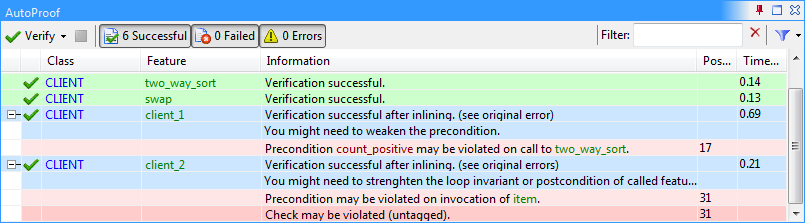
\includegraphics[width=\columnwidth]{images/eve_panel_twostep.png}
\caption{\AutoProof showing feedback of two-step verification.}
\label{fig:two-step-feedback}
\end{figure}


Routine \e{client_2} calls \e{two_way_sort} on a four-element array and checks that its first element is \e{False} after the call.
Modular verification cannot prove this assertion: \e{two_way_sort} has no postcondition, and hence its effects within \e{client_2} are undefined.
The second verification attempt inlines \e{two_way_sort} and unrolls the loop four times (since it notices that the call is on a four-element array); this proves that the first array element is \e{False} after the call (first line in Table~\ref{tab:two-step-unroll-summary}).
In all, \e{two_way_sort} is not to blame because its implementation works correctly for \e{client_2}.
As summarized in the second line of Table~\ref{tab:two-step-inline-summary}, the user can either just be happy with the result or endeavor to write down a suitable postcondition for \e{two_way_sort} so that the correctness proof can be generalized to arrays of arbitrary length.

Suppose we provide a postcondition that specifies sortedness using Eiffel's across syntax:
\begin{erunning}
across 1..(a.count-1) as k all
				(a[k] = a[k+1]) or (a[k] /= a[k+1] and a[k] = False)
\end{erunning}
Modular verification of \e{two_way_sort} fails to prove this postcondition because the loop invariant at line~\ref{l:loop-inv} does not say anything about the array content.
Two-step verification makes a second attempt where it unrolls the loop a finite number of times, say 5, and inlines \e{swap}.
The situation is in the second entry of Table~\ref{tab:two-step-unroll-summary}: we cannot verify that the arbitrary bound of five iterations generally holds (that is $j - i + 1 \leq 5$ holds before the loop), but the success of unrolling in this limited case suggests that \e{two_way_sort}'s implementation is correct.
If we want to get to a general proof, we should improve the loop invariant, and this is precisely the suggestion that two-step verification brings forward.



%============================================================================
\subsection{Evaluation}\label{evaluation}
%============================================================================

The examples of the previous sections have demonstrated the kind of feedback two-step verification provides.
This section contains a preliminary evaluation of the scalability of two-step verification, and of its benefits in terms of reduced annotation burden.

\begin{table}[ht]
\footnotesize
\setlength{\tabcolsep}{3.8pt}
\centering 
\begin{tabular}{ r l r| rrrr r r@{.}l | rrrr r r@{.}l |}
& & & \multicolumn{7}{c|}{\textsc{two-step}} &  \multicolumn{7}{c|}{\textsc{modular}} \\
& & & {\scriptsize $P$} & {\scriptsize $Q$} & {\scriptsize $I$} & {\scriptsize $A$} & & \multicolumn{2}{c|}{} & {\scriptsize $P$} & {\scriptsize $Q$} & {\scriptsize $I$} & {\scriptsize $A$} & \multicolumn{3}{c|}{} \\[-2pt]
& & \textit{code} & \multicolumn{4}{c}{\textit{spec}} & \textit{Boogie} & \multicolumn{2}{c|}{\textit{time}} & \multicolumn{4}{c}{\textit{spec}} & \textit{Boogie} & \multicolumn{2}{c|}{\textit{time}} \\
\hline
   &          &    &  {\scriptsize 1} & {\scriptsize 3} & {\scriptsize 0} & {\scriptsize 0}   & \multicolumn{3}{c|}{} &  {\scriptsize 1} & {\scriptsize 3} & {\scriptsize 4} & {\scriptsize 0} & \multicolumn{3}{c|}{} \\[-3pt]
1. & Maximum  & 32 & \multicolumn{4}{c}{\ 4} & 1541 \ & 2&06 & \multicolumn{4}{c}{\ 8} & 712 \ & 1&05 \\
   &          &    &  {\scriptsize 3} & {\scriptsize 1} & {\scriptsize 0} & {\scriptsize 0}   & \multicolumn{3}{c|}{} &  {\scriptsize 3} & {\scriptsize 1} & {\scriptsize 5} & {\scriptsize 0} & \multicolumn{3}{c|}{} \\[-3pt]
2. & Sum and Max  & 32 & \multicolumn{4}{c}{\ 4} & 1619 \ & 2&18 & \multicolumn{4}{c}{\ 9} & 720 \ & 1&04 \\
   &          &    &  {\scriptsize 2} & {\scriptsize 1} & {\scriptsize 0} & {\scriptsize 0}   & \multicolumn{3}{c|}{} &  {\scriptsize 2} & {\scriptsize 1} & {\scriptsize 5} & {\scriptsize 0} & \multicolumn{3}{c|}{} \\[-3pt]
3. & Two-way Sort  & 44 & \multicolumn{4}{c}{\ 3} & 1803 \ & 2&35 & \multicolumn{4}{c}{\ 8} & 742 \ & 1&06 \\
   &          &    &  {\scriptsize 2} & {\scriptsize 1} & {\scriptsize 0} & {\scriptsize 0}   & \multicolumn{3}{c|}{} &  {\scriptsize 2} & {\scriptsize 1} & {\scriptsize 10} & {\scriptsize 0} & \multicolumn{3}{c|}{} \\[-3pt]
4. & Dutch Flag  & 45 & \multicolumn{4}{c}{\ 3} & 1955 \ & 2&94 & \multicolumn{4}{c}{\ 13} & 786 \ & 1&14 \\
   &          &    &  {\scriptsize 3} & {\scriptsize 4} & {\scriptsize 0} & {\scriptsize 0}   & \multicolumn{3}{c|}{} &  {\scriptsize 3} & {\scriptsize 4} & {\scriptsize 7} & {\scriptsize 0} & \multicolumn{3}{c|}{} \\[-3pt]
5. & LCP  & 30 & \multicolumn{4}{c}{\ 7} & 1585 \ & 2&10 & \multicolumn{4}{c}{\ 14} & 730\ & 1&05 \\
\hline
   &          &    &  {\scriptsize 0} & {\scriptsize 0} & {\scriptsize 0} & {\scriptsize 7}   & \multicolumn{3}{c|}{} &  {\scriptsize 5} & {\scriptsize 13} & {\scriptsize 5} & {\scriptsize 7} & \multicolumn{3}{c|}{} \\[-3pt]
6. & Priority queue & 119 & \multicolumn{4}{c}{\ 7} & 2896 \ & 3&35 & \multicolumn{4}{c}{\ 30} & 1088 \ & 1&56 \\
   &          &    &  {\scriptsize 0} & {\scriptsize 0} & {\scriptsize 0} & {\scriptsize 11}   & \multicolumn{3}{c|}{} &  {\scriptsize 7} & {\scriptsize 18} & {\scriptsize 4} & {\scriptsize 11} & \multicolumn{3}{c|}{} \\[-3pt]
7. & Deque & 127 & \multicolumn{4}{c}{\ 11} & 1856 \ & 2&51 & \multicolumn{4}{c}{\ 40} & 1230 \ & 1&59 \\
   &          &    &  {\scriptsize 0} & {\scriptsize 0} & {\scriptsize 0} & {\scriptsize 1}   & \multicolumn{3}{c|}{} &  {\scriptsize 2} & {\scriptsize 3} & {\scriptsize 0} & {\scriptsize 1} & \multicolumn{3}{c|}{} \\[-3pt]
8. & Binary Search  & 48 & \multicolumn{4}{c}{\ 1} & 2479 \ & 3&21 & \multicolumn{4}{c}{\ 6} & 672 \ & 0&99 \\
\hline \hline
   &          &    &  {\scriptsize \textit{11}} & {\scriptsize \textit{10}} & {\scriptsize \textit{0}} & {\scriptsize \textit{19}}   & \multicolumn{3}{c|}{} &  {\scriptsize \textit{25}} & {\scriptsize \textit{44}} & {\scriptsize \textit{40}} & {\scriptsize \textit{19}} & \multicolumn{3}{c|}{} \\[-3pt]
& \textit{Total} & \textit{477} & \multicolumn{4}{c}{\ \textit{40}} & \textit{15734} \ & \textit{20}&\textit{70} & \multicolumn{4}{c}{\ \textit{128}} & \textit{6680} \ & \textit{9}&\textit{48}
\end{tabular}
\caption{Comparison of two-step and modular verification on selected examples.}
\label{tab:two-step:examples}
\end{table}


Table~\ref{tab:two-step:examples} lists the example programs.
The first labeled column after the program name contains the size of the implementation (not counting specification elements) in lines of code.
The rest of the table is split in two parts: the first one contains data about two-step verification; the second one the same data about modular verification.
The data reported includes: the amount of specification necessary to successfully verify the example (number of annotations, split into preconditions $P$, postconditions $Q$, invariants $I$ (loop invariants in examples 1--5; class invariants in examples 6--8), and intermediate assertions $A$); the size (in lines) of the Boogie code generated by AutoProof; and the time in seconds.
Two-step verification includes modular verification as first step, but normally requires less specification to be successful; correspondingly, the Boogie code and the time in the first part of the table sum up both steps.
 


The examples include: 
(1)~finding the maximum in an array, from the COST 2011 verification competition~\cite{BORMER11};
(2)~computing maximum and sum of the elements in an array, from the VSTTE 2010 verification competition~\cite{KLEBANOV11};
(3)~the two-way sort algorithm of Section~\ref{sec:ap-overview}, from the VSTTE 2012 verification competition~\cite{FILLIATRE12};
(4)~Dikstra's Dutch national flag algorithm~\cite{DIJKSTRA76};
(5)~computing the longest common prefix of two sequences, from the FM 2012 verification competition~\cite{HUISMAN12};
(6)~a priority queue implementation, from Tinelli's verification course~\cite{TINELLI2011}; 
(7)~a double-ended queue~\cite[Vol.~1, Sec.~2.2.1]{KNUTH11}; and
(8)~the binary search algorithm of Section~\ref{sec:ap-overview}, from the software verification benchmarks~\cite{VSI08}. 




In the experiments with the algorithms 1--5, two-step verification succeeds with loop unrolling of depth $n=6$, which corresponds to input arrays of the same length.
The outcome suggests either to use the unrolled loop, for inputs of bounded length; or to write a suitable loop invariant.
A correct loop invariant is necessary for modular verification alone to succeed, in which case the proof generalizes to arrays of arbitrary length.
We prove the following postconditions: (1) the output is the array maximum; (2) the output sum is less than or equal to the output maximum times the array length; (3) sortedness of the output, as formalized in Section~\ref{sec:examples-two-step}; (4) the output is partitioned in the three flag colors; (5) the output is the longest common prefix of the input array.



In the experiments 6--8 we verify \emph{clients} of the queue, double-ended queue, and binary search, which call some routines and then formalize their expectations on the result with \e{assert}s after the call.
The called routines have no specification (in particular, no postcondition); two-step verification verifies the clients using inlining of the callee, and suggests to add postconditions to generalize the proofs.
The postconditions are necessary for modular verification alone to succeed.

The evaluation suggests that two-step verification can check the implementation even when little or no specification is given; its feedback may then help write the necessary specifications to generalize proofs for modular verification.


The runtime overhead of performing two verification steps instead of one is roughly linear in all examples; in fact, unrolling and inlining blow up mainly in the presence of recursion.
To better assess how they scale, we have repeated two-step verification of examples 3 (using unrolling) and 6 (using inlining in the presence of recursion) for increasing value of the bound $n$.
Table~\ref{tab:two-step:blowup} shows the results in terms of size of the generated Boogie code (in lines) and time necessary to verify it (in seconds).
Unrolling scales gracefully until about $n=10$; afterward, the time taken by Boogie to verify increases very quickly, even if the size of the Boogie code does not blow up.
Inlining is more sensitive to the bound, since the size of the inlined code grows exponentially due to the conditional branch in \e{binary_search}'s body; the time is acceptable until about $n = 7$.
Notice that the heuristics for the choice of $n$ discussed in Section~\ref{sec:bounds} would generate running times in the order of tens of seconds, thus enforcing a reasonable responsiveness.



\begin{table}[th]
\centering 
\begin{tabular}{r| r r@{.}l | r r@{.}l }
	&
	\multicolumn{3}{c|}{\textsc{unrolling}}
	&
	\multicolumn{3}{c}{\textsc{inlining}}
	\\
	\textit{inlining/unrolling depth} $n$ &
	\textit{Boogie} 
	&
	\multicolumn{2}{c|}{\textit{time}}
	&
	\textit{Boogie} 
	&
	\multicolumn{2}{c}{\textit{time}}
	\\
  \hline
 3 & 864 & 1&07 & 1201 & 1&44 \\
 4 & 937 & 1&13 & 1822 & 2&26 \\
 5 & 1010 & 1&21 & 3054 & 4&23 \\
 6 & 1083 & 1&32 & 5518 & 10&93 \\
 7 & 1156 & 1&52 & 10446 & 30&64 \\
 8 & 1229 & 2&03 & 20302 & 112&32 \\
 10 & 1375 & 4&26 & \multicolumn{1}{c}{--} & \multicolumn{2}{c}{--} \\
 13 & 1594 & 37&52 & \multicolumn{1}{c}{--} & \multicolumn{2}{c}{--} \\
 15 & 1667 & 253&30 & \multicolumn{1}{c}{--} & \multicolumn{2}{c}{--}
\end{tabular}
\caption{Scalability of unrolling and inlining on examples 3 and 6 from Table~\ref{tab:two-step:examples}.}
\label{tab:two-step:blowup}
\end{table}






%============================================================================
\subsection{Related Work}\label{related-work}
%============================================================================

The steadily growing interest for techniques and tools that make verification more approachable indicates how some of the most glaring hurdles to the progress of formal methods lie in their applicability.
Tools such as Dafny~\cite{LEINO10}, Spec\#~\cite{BARNETT05}, VCC~\cite{COHEN09}, ESC/Java2~\cite{COK05,JAMES10}, and Why3~\cite{BOBOT11} define the state of the art in static program verification.
Their approaches rely on accurate specifications, which are not easy to write and get right.

One way to ameliorate this situation is inferring specifications automatically using static~\cite{CHANG05,KOVACS09,FURIA10} or dynamic~\cite{ERNST01,WEI11,WASYLKOVSKI11} techniques.
Specifications dynamically inferred are based on a finite number of executions, and hence may be unsound; this makes them unsuitable for use in the context of static verification.
Static techniques can infer sound specifications from the program text; these are useful to document existing implementations, to discover auxiliary assertions (such as loop invariants), or for comparison with specifications independently written, but proving an implementation correct against a specification inferred from it is mostly a vacuous exercise.

The simple implicit contracts that we use in our approach express well-formedness properties of the input program, which are tacitly assumed by programmers reasoning informally about it; therefore, there is no risk of circularity.
Some static verifiers use mathematical integers or assume purity of specification functions to have well-formedness by construction; a risk is that, when they are applied to real programming languages, the corresponding semantic gap may leave some errors go unnoticed.
ESC/Java2, for example, does not check for overflows~\cite{KINIRY06}, nor if specification expressions are executable (for example, null-dereferencing could happen when evaluating a precondition).
The Dafny verifier checks well-formedness of pre- and postconditions, and may consequently require users to add explicit contracts to satisfy well-formedness. Our implicit contracts are instead added and checked automatically, without requiring users to explicitly write them.
In this sense, they are similar to approaches such as VCC, which models the semantics of the C programming language as precisely as possible.

Besides inferring specifications, another approach to facilitate formal verification is combining complementary verification techniques.
CEGAR model-checking~\cite{BEYER07}, for example, uses model-checking exhaustive verification techniques on approximate program models, combined with a form of symbolic execution to determine whether the failed verification attempts are indicative of real implementation errors or only a figment of an imprecise abstraction.
Tools such as DSD-Crasher~\cite{CSALLNER08} and our EVE~\cite{TSCHANNEN11} integrate testing and static checking to find when the errors reported by the latter are spurious.
Collaborative verification~\cite{CHRISTAKIS12} is also based on the combination of testing and static verification, and on the explicit formalization of the restrictions of each tool used in the combination.
Two-step verification also integrates the results of different techniques, with the main purpose of improving error reporting and reducing the number of annotations needed, rather than complementing the limitations of specific techniques.

The Spec\# system includes a verification debugger~\cite{MOSKAL11} to inspect error models when verification fails; more recently, an interpreter for Boogie programs~\cite{POLIKARPOVA13} can help find the sources of failed verification attempts.
Debuggers for verification can be quite useful in practice, but achieve a lesser degree of automation than two-step verification, since users need to manually inspect and understand the error models using the debugger.



%############################################################################
\section{Polymorphic Calls}
\label{sec:m-polymorphic}
%############################################################################


The redefinition of a routine $r$ in a descendant class can \emph{strengthen} $r$'s original postcondition by adding an \e{ensure then} clause, which conjoins the postcondition in the precursor.
The example in Figure~\ref{example-exp} illustrates a difficulty occurring when reasoning about postcondition strengthening in the presence of polymorphic types.
The deferred (abstract) class \e{EXP} models nonnegative integer expressions and provides a routine \e{eval} to evaluate the value of an expression object; even if \e{eval} does not have an implementation in \e{EXP}, its postcondition specifies that the evaluation always yields a nonnegative value stored in attribute \e{last_value}, which is set as side effect.
Classes \e{CONST} and \e{PLUS} respectively specialize \e{EXP} to represent integer (nonnegative) constants and addition.
Class \e{ROOT} is a client of the other classes, and its \e{main} routine attaches an object of subclass \e{CONST} to a reference with static type \e{EXP}, thus exploiting polymorphism.
Similar issues occur when a descendant class \emph{weakens} a some routine $r$'s precondition with an \e{require else} clause.


\begin{figure}[!ht]
\begin{tabular}{ll}

{\begin{erunning}
deferred class EXP
feature
	last_value: INTEGER
	eval
		deferred
		ensure
			last_value >= 0
		end
end
 #\ # 
 #\ # 
 #\ # 
 #\ # 
\end{erunning}}
&
\hspace{5mm}
{\begin{erunning}
class PLUS inherit EXP feature 
	left, right: EXP
	eval do
			left.eval; right.eval
			last_value := left.last_value + 
						  right.last_value
		ensure then
			last_value = left.last_value + 
						 right.last_value
		end
invariant
	left /= right /= Current
end
\end{erunning}}
\vspace{5mm}
\\
{\begin{erunning}
class CONST inherit EXP
feature 
	value: INTEGER
	eval do
			last_value := value
		ensure then
			last_value = value
		end
invariant
	value >= 0
end
\end{erunning}}
&
\hspace{5mm}
{\begin{erunning}
class ROOT
feature    
	main
		local
				e: EXP
		do
			e := create {CONST}.make (5);
			e.eval
			check e.last_value = 5 end    
		end
end 
\end{erunning}}

\\

\end{tabular}
\caption{Nonnegative integer expressions.}\label{example-exp}
\end{figure}

The verification goal is proving that, after the invocation $e.eval$ (in class \e{ROOT}), \e{eval}'s postcondition in class \e{CONST} holds, which subsumes the \e{check} statement in the caller.
Reasoning about the invocation only based on the static type \e{EXP} of the target \e{e} guarantees the postcondition \e{last_value >= 0}, which is however too weak to establish that \e{last_value} is exactly 5.

Other approaches, such as M\"uller's~\cite{MUELLER02}, have targeted these issues in the context of Hoare logics, but they usually are unsupported by automatic program verifiers.
In particular, with the Boogie translation of polymorphic assignment implemented in Spec\#, the assertion \e{check e.last_value = 5 end} in class \e{ROOT} can be verified only if \e{eval} is declared \emph{pure}; \e{eval} is, however, not pure.
The Spec\# methodology selects the pre and postconditions according to static types for non-pure routines: the call \e{e.eval} only establishes \e{e.last_value >= 0}, not the stronger \e{e.last_value = 5} that follows from \e{e}'s dynamic type \e{CONST}, unless an explicit cast redefines the type \e{CONST}.
The rest of the section describes the solution implemented in \AutoProof, which handles contracts of redefined routines.




%============================================================================
\subsection{Polymorphism in Boogie}
%============================================================================

The Boogie translation implemented in \AutoProof can handle polymorphism appropriately even for non-pure routines; it is based
on a methodology for agents~\cite{NORDIO10} and on a methodology for pure routines~\cite{DARVAS07,LEINO08b}.
The rest of the section discusses how to translate postconditions and preconditions of redefined routines in a way that accommodates polymorphism, while still supporting modular reasoning.


%----------------------------------------------------------------------------
\subsubsection{Postconditions}
%----------------------------------------------------------------------------

The translation of the postcondition of a routine $r$ of class $X$ with result type $T$ (if any) relies on an auxiliary function \b{post.X.r}:
\begin{brunning}
function post.X.r (h1, h2: HeapType; c: ref; res: T) returns (bool);
\end{brunning}
which predicates over two heaps (the pre and post-states in $r$'s postcondition), a reference \b{c} to the current object, and the result \b{res}.
$r$'s postcondition in Boogie references the function \b{post.X.r}, and includes the translation $\nabla_{post}(X.r)$ of $r$'s postcondition clause syntactically declared in class \e{X}:\footnote{The translation differs for calls to \e{Precursor} (\lstinline[language=Java]|super| in Java and \lstinline[language={[Sharp]C}]|base| in C\#).}
\begin{brunning}
procedure X.r (Current: ref) returns (Result: T);
  free ensures post.X.r (Heap, old(Heap), Current, Result);
  ensures $\nabla_{post}(X.r)$;
\end{brunning}
\b{post.X.r} is a \b{free ensures}, hence it is ignored when proving $r$'s implementation and is only necessary to reason about usages of $r$.

The function \b{post.X.r} holds only for the type $X$; for each class $Y$ which is a descendant of $X$ (and for $X$ itself), an axiom links $r$'s postcondition in $X$ to $r$'s strengthened postcondition in $Y$:
\begin{brunning}
axiom (forall h1, h2: HeapType; c: ref; r: T ::
    type_of(c) <: Y ==> (post.X.r(h1, h2, c, r) ==> #$\nabla_{post}(Y.r)$#));
\end{brunning}
The function \b{type_of} returns the type of a given reference; hence the postcondition predicate $post.X.r$ implies an actual postcondition $\nabla_{post}(Y.r)$ according to $c$'s dynamic type. 

In addition, for each redefinition of $r$ in a descendant class $Z$, 
the translation defines a fresh Boogie procedure $Z.r$ with 
corresponding postcondition predicate $post.Z.r$ and axioms 
for all of $Z$'s descendants.


%----------------------------------------------------------------------------
\subsubsection{Preconditions}
%----------------------------------------------------------------------------


Eiffel also supports \emph{weakening of preconditions}. Therefore, the precondition
of a routine can also depend on the dynamic type. We use a similar
translation as for the postcondition. Given a routine $r$ of type $X$, 
a precondition predicate is generated and used in the signature 
of the generated Boogie procedure:
\begin{brunning}
function pre.X.r(h: HeapType; c: ref) returns (bool);
\end{brunning}
which predicates over one heap and a reference \e{c} to the current object.
\e{r}'s precondition in Boogie references the function \b{pre.X.r}, and it includes the translation $\nabla_{pre}(X.r)$ of $r$'s precondition originally declared in class $X$:
\begin{brunning}
procedure X.r (Current: ref) returns (Result: T);
	requires pre.X.r(Heap, Current);
	free requires #$\nabla_{pre}(X.r)$#
\end{brunning}
Conversely to the postcondition, establishing $r$'s precondition is a responsibility of callers of $r$; clients have to establish the precondition determined by the dynamic type---captured by the function \b{pre.X.r}---, whereas the precondition originally given in $X$ is given as a \b{free requires} and is only used to prove $r$'s implementation.
\begin{brunning}
axiom (forall h: HeapType; c: ref ::
		type_of(c) <: Y ==> (#$\nabla_{pre}(Y.r)$# ==> pre.X.r(h, c)));
\end{brunning}
To establish \b{pre.X.r}, it is enough to establish any of the clauses $\nabla_{pre}(Y.r)$.


\begin{bfigure}[p]{Simplified Boogie translation of the Eiffel classes in Figure~\ref{example-exp}.}{fig-exp-boogie}
function post.EXP.eval(h1, h2: HeapType; c: ref) returns (bool);

procedure EXP.eval(current: ref); #\label{l:exp:boogie:a}#
	free ensures post.EXP.eval(Heap, old(Heap), current); #\label{l:exp:boogie:k}#
	ensures Heap[current, last_value] >= 0;
	// other specification omitted #\label{l:exp:boogie:b}#

axiom (forall h1, h2: HeapType; o: ref :: #\label{l:exp:boogie:c}#
	type_of(o) <: EXP ==> 
	(post.EXP.eval(h1, h2, o) ==> (h1[o, last_value] >= 0)) ); #\label{l:exp:boogie:d}#
axiom (forall h1, h2: HeapType; o: ref :: #\label{l:exp:boogie:e}#
	type_of(o) <: CONST ==> 
	(post.EXP.eval(h1, h2, o) ==> h1[o, last_value] == h1[o, value]) ); #\label{l:exp:boogie:f}#
axiom (forall h1, h2: HeapType; o: ref :: #\label{l:exp:boogie:g}#
	type_of(o) <: PLUS ==> 
	(post.EXP.eval(h1, h2, o) ==> (h1[o, last_value] == 
		h1[h1[o, left], last_value] + h1[h1[o, right], last_value])) ); #\label{l:exp:boogie:h}#

implementation ROOT.main (Current: ref) {
		var e: ref;
	entry:
		// translation of: #\textbf{create} \{\textit{CONST}\} \textit{e.make} (5)#
		havoc e;
		assume Heap[e, allocated] == false;
		Heap[e, allocated] := true;
		assume type_of(e) == CONST; #\label{l:exp:boogie:i}#
		call CONST.make(e, 5);
		// translation of: #\textit{e.eval}#
		call EXP.eval(e);
		// translation of: #\textbf{check} \textit{e.last\_value} = 5 \textbf{end}#
		assert Heap[e, last_value] == 5; #\label{l:exp:boogie:j}#
		return;
}
\end{bfigure} 



%============================================================================
\subsection{An Example of Polymorphism with Postconditions}
%============================================================================

Figure~\ref{fig-exp-boogie} shows the essential parts of the Boogie translation of the example in Figure~\ref{example-exp}. 
The translation of routine \e{eval} in lines \ref{l:exp:boogie:a}--\ref{l:exp:boogie:b} references the function \b{post.EXP.eval}; the axioms in lines \ref{l:exp:boogie:c}--\ref{l:exp:boogie:h} link that function to $r$'s postcondition in \e{EXP} (lines \ref{l:exp:boogie:c}--\ref{l:exp:boogie:d}) and to the additional postcondition introduced in \e{CONST} (lines \ref{l:exp:boogie:e}--\ref{l:exp:boogie:f}) and \e{PLUS} (lines \ref{l:exp:boogie:g}--\ref{l:exp:boogie:h}) for the same routine.

The rest of the figure shows the translation of the client class \e{ROOT}. To verify the assertion on line~\ref{l:exp:boogie:j} the verifier will use the fact that the reference \b{e} is of type \e{CONST} (line~\ref{l:exp:boogie:i}), that the postcondition function \b{post.EXP.eval} holds thanks to the postcondition of \e{eval} (line~\ref{l:exp:boogie:k}), and the axiom generated for the specific subtype (line~\ref{l:exp:boogie:e}). With this information, the verifier can establish that the assertion holds.


%============================================================================
\subsection{Related Work}
%============================================================================


Spec\#~\cite{BARNETT05} uses dynamic postconditions for pure functions, taking the dynamic object type into account. In contrast, our approach works for functions that have side-effects and for adaptations of preconditions as well.

Rapid Type Analysis~\cite{BACON96} can be used to determine all possible types of an object at a call site.
The algorithm analyses the full system and is therefore non-modular.
For local variables that are only available in the context of a single routine this analysis would be suitable even for modular verification.

Using abstract interpretation~\cite{COUSOT77}, Rapid Atomic Type Analysis~\cite{LOGOZZO10} can be used to infer precise types of numeric variables, even for dynamically typed languages.


%############################################################################
\section{Exceptions}
\label{sec:m-exceptions}
%############################################################################

Eiffel's exception handling mechanism is different from most other object-oriented programming languages such as C\# and Java.\footnote{Other work has formalized the semantics of Java exceptions~\cite{MUELLER07} and compared it against Eiffel's~\cite{NORDIO09}.}
This section presents Eiffel's exception mechanism (Section~\ref{sec:m-exceptions:eiff-except-mech}), discusses how to annotate exceptions (Section~\ref{sec:m-exceptions:spec-except}), and describes the translation of Eiffel's exceptions to Boogie (Section~\ref{sec:m-exceptions:translation-boogie}) with the help of an example and a small case study (Section~\ref{sec:m-exceptions:example}).

The methodology described here applies to the Eiffel exception mechanism as described in the Eiffel ECMA standard~\cite{ECMA367}.
Since the Eiffel compilers existing today are still using the old exception mechanism, this methodology is not implemented in \AutoProof.


%============================================================================
\subsection{How Eiffel Exceptions Work} \label{sec:m-exceptions:eiff-except-mech}
%============================================================================


Eiffel exception handlers are specific to each routine, where they occupy an optional \e{rescue} clause, which follows the routine body (\e{do}).
A routine's \e{rescue} clause is ignored whenever the routine body executes normally. 
If, instead, executing the routine body triggers an exception, control is transferred to the  \e{rescue} clause for exception handling.
The exception handler will try to restore the object state to a condition where the routine can execute normally.
To this end, the body can run more than once, according to the value of an implicit variable \e{Retry}, local to each routine: when the execution of the handler terminates, if \e{Retry} has value \e{True} the routine body is run again, otherwise \e{Retry} is \e{False} and the pending exception propagates to the \e{rescue} clause of the caller routine\footnote{This is how Eiffel's exception mechanism is described in the current Eiffel specification draft by the Eiffel ECMA committee. The main Eiffel compiler is using the older exception mechanism, where \e{retry} is a statement that immediately exits the rescue clause}.

Figure~\ref{fig:exceptions-eiffel} illustrates the Eiffel exception mechanism with an example. 
The routine \e{attempt_transmission} tries to transmit a message by calling \e{unsafe_transmit}; if the latter routine terminates normally, then also \e{attempt_transmission} terminates normally without executing the \e{rescue} clause.
On the contrary, an exception triggered by \e{unsafe_transmit} transfers control to the \e{rescue} clause, which re-executes the body \e{max_attempts} times; if all the attempts fail to execute successfully, the attribute \e{failed} is set and the exception propagates. 

\begin{efigure}[ht]{An Eiffel routine with exception handler.}{fig:exceptions-eiffel}
attempt_transmission (m: STRING)
	local
		failures: INTEGER
	do
		failed := False
		unsafe_transmit (m)
	rescue
		failures := failures + 1
		if failures < max_attempts then
			Retry := True
		else
			failed := True
		end
	end
\end{efigure}




%============================================================================
\subsection{Specifying Exceptions} \label{sec:m-exceptions:spec-except}
%============================================================================


The postcondition of a routine with \e{rescue} clause specifies the program state both after normal termination and when an exception is triggered. 
The two post-states are in general different, hence we introduce a global Boolean variable \e{ExcV}, which is \e{True} if and only if the routine has triggered an exception.
Using this auxiliary variable, specifying postconditions of routines with exception handlers is straightforward.
For example, the postcondition of routine \e{attempt_transmission} in Figure~\ref{fig:exceptions-eiffel} says that \e{failed} is \e{False} if and only if the routine executes normally:

\begin{erunning}
attempt_transmission (m: STRING)
	ensure
		ExcV implies failed
		not ExcV implies not failed
\end{erunning} 

The example also shows that the execution of a \e{rescue} clause behaves as a loop: a routine \e{r} with exception handler \e{r do$\ s_1\ $rescue$\ s_2\ $end} behaves as the loop that first executes $s_1$ unconditionally, and then repeats $s_2 \,;\, s_1$ until $s_1$ triggers no exceptions or \e{Retry} is \e{False} after the execution of $s_2$ (in the latter case, $s_1$ is not executed anymore).
To reason about such implicit loops, we introduce a \emph{rescue invariant}~\cite{NORDIO09-2,NORDIO08}; the rescue invariant holds after the first execution of $s_1$ and after each execution of $s_2\,;\,s_1$.
A suitable rescue invariant of routine \e{attempt_transmission} is:

\begin{erunning}
rescue invariant
	not ExcV implies not failed
	(failures < max_attempts) implies not failed
\end{erunning} 


%============================================================================
\subsection{Eiffel Exceptions in Boogie} \label{sec:m-exceptions:translation-boogie}
%============================================================================

The auxiliary variable \e{ExcV} becomes a global variable in Boogie, so that every assertion can reference it.
The translation also introduces an additional precondition \boogie{ExcV = false} for every translated routine, because normal calls cannot occur when exceptions are pending, and adds ExcV to the modifies clause of every procedure.
Then, a routine with body $s_1$ and rescue clause $s_2$ becomes in Boogie:

\begin{brunning}
	$\tr{s_1, excLabel}$
excLabel:
	while (ExcV) 
	invariant $\tr{I_{rescue}}$;
	{
		ExcV := false;
		Retry := false;
		$\tr{s_2, endLabel}$  
		if (!Retry) { ExcV := true; goto endLabel; }
		$\tr{s_1, excLabel}$
	}
endLabel:
\end{brunning} 

\noindent
where $\tr{s, l}$ denotes the Boogie translation $\tr{s}$ of the instruction $s$, followed by a jump to label $l$ if $s$ triggers an exception:
\begin{equation*}
\tr{s, l} \ =\ \begin{cases}
  \tr{s', l} \,;\,\tr{s'', l} &  \text{if } s \text{ is the compound }s'\,;\,s'' \\
  \tr{s} \,;\, \text{\b{if (ExcV) $\,$\{goto l;\}}}  &  \text{otherwise}
 \end{cases}
\end{equation*}

Therefore, when the body $s_1$ triggers an exception, \b{ExcV} is set and the execution enters the rescue loop. %, which handles the exception.
On the other hand, an exception that occurs in the body of $s_2$ jumps out of the loop and to the end of the routine.

The exception handling semantics is only superficially similar to having control-flow breaking instructions such as \emph{break} and \emph{continue}---available in languages other than Eiffel---inside standard loops: the program locations where the control flow diverts in case of exception are implicit, hence the translation has to supply a conditional jump after every instruction that might trigger an exception.
This complicates the semantics of the source code, and correspondingly the verification of Boogie code translating routines with exception handling. 
This makes it not only harder for the verifier to prove a routine, but also for the programmer to understand the exact semantics of the code.


%============================================================================
\subsection{Example and Case Study} \label{sec:m-exceptions:example}
%============================================================================


Figure~\ref{fig:exceptions-boogie} shows the translation of the example in Figure~\ref{fig:exceptions-eiffel}. 
To simplify the presentation, Figure~\ref{fig:exceptions-boogie} renders the attributes \e{max_attempts}, \e{failed}, and \e{transmitted} (set by \e{unsafe_transmit}) as variables rather than locations in a heap map.
The loop in lines~\ref{loop-begin}--\ref{loop-end} maps the loop induced by the \e{rescue} clause, and its invariant (lines \ref{inv1} and \ref{inv2}) is the rescue invariant.

\begin{bfigure}[hp]{Boogie translation of the Eiffel routine in Figure~\ref{fig:exceptions-eiffel}.}{fig:exceptions-boogie}
var max_attempts: int; 
var failed: bool; 
var transmitted: bool;

procedure unsafe_transmit (m: ref);
	free requires ExcV == false;
	modifies ExcV, transmitted;
	ensures ExcV <==> !transmitted;

procedure attempt_transmission (m: ref);
	free requires ExcV == false;
	modifies ExcV, transmitted, max_attempts, failed;
	ensures ExcV <==> failed;

implementation attempt_transmission (m: ref)
{
		var failures: int;
		var Retry: bool;  
	entry:
		failures := 0; Retry := false; failed := false;
		call unsafe_transmit (m); if (ExcV) { goto excL; }       
	excL:
			while (ExcV) #\label{loop-begin}#
			invariant ! ExcV ==> ! failed; #\label{inv1}#
			invariant (failures < max_attempts) ==> ! failed; #\label{inv2}#
			{    
				ExcV := false; Retry := false;
				failures := failures + 1; 
				if (failures < max_attempts) {
					Retry := true;
				} else {
					failed := true;
				}
				if (! Retry) {ExcV := true; goto endL;}    
				failed := false
				call unsafe_transmit (m); if (ExcV) { goto excL; }
			}  #\label{loop-end}#
	endL:
		return;
}     
\end{bfigure}

We have done a small case study with a set of routines presented in Meyer's book~\cite{MEYER97} when describing Eiffel exceptions and a second set of classes that are part of the EiffelStudio compiler. To verify them, we extended the original contracts with postconditions to express the behavior when exceptions are triggered, and with rescue invariants. The translation of the examples to Boogie was done by hand, as the described methodology is not implemented in our verifier. The results of the case study are summarized in the following table:

\begin{center}
\footnotesize
\begin{tabular}{ l  c c c c c }
  \textsc{Example name} \ \ & \textsc{Classes}\ \ & \textsc{LOC\newline Eiffel}\ \ \ \ & \textsc{LOC\newline Boogie}\ \ \ \ & \textsc{Time [s]} \\ \hline
  Textbook OOSC2   & 1 & 106 & 481 & 2.33  \\
  Runtime ISE      & 4 & 203 & 561 & 2.32 \\
\end{tabular}
\end{center}

The most difficult part of verifying these example was inventing rescue invariants. Even when the examples are simple, the rescue invariants may be subtle, because not only is the loop to reason about implicit, but they also have to include clauses both for normal and for exceptional termination.



%============================================================================
\subsection{Related Work} \label{sec:m-exceptions:related-work}
%============================================================================

Other object-oriented languages such as Java or C\# have exception mechanisms that allow to catch exceptions for arbitrary code blocks. If exceptions are not catched, they are thrown to the calling context. This execution model---in absence of unusual situations like using jump instructions in the catch block---does not introduce implicit loops and therefore does not need exception invariants.

To deal with exceptional executions of routines, Java-based verifiers such as Krakatoa~\cite{MARCHE05} and OpenJML~\cite{COK11} allow postconditions for the case of an uncaught exception. This is equivalent to using an exception value to conditionally trigger some postconditions in the regular case and other postconditions in the exceptional case.

Spec\# provides a special annotation to signal to clients of a routine which exceptions will be triggered if the caller does not fulfill particular precondition clauses~\cite{LEINO04b}



\imagechapter
%############################################################################
\chapter{Conclusions and Future Work}
\label{sec:concl_fut}
\chapterimage{images/conclusions}
%############################################################################

%============================================================================
\section{Conclusions}
\label{sec:conclusions}
%============================================================================

This thesis presented work in the area of automated software verification with a focus on usability and tool support.

To combine verification tools in an IDE we have developed a scoring system to aggregate results in a single interface.
The system works by having each tool assign a score for each routine and provide a confidence in the soundness of its own result.
A single routine score computed based on the results and confidence of each tool.
To create a class score, routine scores are combined based on a routine's importance.
The developer can investigate the correctness of the system at different granularity levels: per class, per feature, and per tool result.
A prototype of this system---the \VAssist---has been implemented as part of \EVE combining the output of three diverse tools: \AutoProof, \AutoTest, and \Inspector.
The implementation shows that integration on this abstraction level facilitates the addition of new tools in the system.

With \AutoProof we have developed a state-of-the-art auto-active verifier for a real complex object-oriented language.
\AutoProof supports a powerful methodology for framing and class invariants which make it applicable in practice to idiomatic object-oriented patterns.
In addition, \AutoProof supports a methodology to deal with function objects (agents) and polymorphism.
Integrating two-step verification, implicit contracts, inlining, and unrolling, \AutoProof tries to cater not just to the verification experts but also be accessible for novices.
We have evaluated \AutoProof on a rich collection of benchmark problems, all of which are available in an online repository, with a specific focus on verification challenges and object-oriented patterns.
\AutoProof has also been used to verify full functional correctness of a general-purpose container library.
The results attest \AutoProof's competitiveness among tools in its league on cutting-edge functional verification of object-oriented programs.
We have given an in-depth description of several solutions to verification challenges, highlighting various aspects of using \AutoProof in practice.
It is possible to use \AutoProof for these challenges, although inside knowledge of the back-end verifier is necessary sometimes for a successful verification.

The work on \AutoProof has gone on over several years.
The prototype version was created as a proof-of-concept and used an inflexible design that was difficult to extend.
To ease further development, a new version of \AutoProof was built with usability and extensibility in mind.
The implementation uses clear abstractions and exhibits a solid object-oriented design; \AutoProof offers extension points to integrate new translation from Eiffel to Boogie, as well as facilities to translate Eiffel directly to custom Boogie code.
This allows to build Eiffel libraries with custom Boogie axiomatizations without the need of modifying \AutoProof.
We provide various interfaces for using \AutoProof through a graphical user interface, command-line interface, and online and embedded in websites.

We have developed two-step verification, a technique for improving the feedback of automated verifiers. Two-step verification does a second verification attempt for each failed verification whilst inlining routine calls and unrolling loops. By combining the outcome of both verification attempts the verifier can improve the error reporting in cases where the implementation of the verified routine is correct and the specification has to be adapted. The evaluation of two-step verification has shown that for small to moderate examples the overhead is manageable.

To support the Eiffel programming language more fully, we have proposed methodologies for handling polymorphic calls and the exception mechanism of Eiffel. Our methodology for polymorphism takes advantage of redefined contracts whenever the dynamic type of a dynamically bound reference can be inferred from the context. This is achieved by using uninterpreted functions representing pre- and postconditions that are linked to the concrete specifications of a routine based on the dynamic type. We have presented a translation of Eiffel's peculiar exception mechanism to Boogie. Routines that trigger exceptions need an additional postcondition to specify the routine's effect in case of an exception and, since the exception mechanism introduces an implicit loop, a rescue invariant is necessary to reason about the exceptional case.



%============================================================================
\section{Future Work}
\label{sec:futurework}
%============================================================================


%----------------------------------------------------------------------------
\subsubsection{Integrating suggestion tools}
%----------------------------------------------------------------------------

Our tool integration in \EVE has been limited to verification and analysis tools. Another category of tools that developers benefit from are \emph{contract inference tools} and \emph{fixing tools} such as Daikon~\cite{ERNST07} or \AutoFix~\cite{PEI11,PEI14}. Although these tools cannot be integrated directly with the scoring system implemented in the \VAssist, the information collected from the verification tools can be used to target inference and fixing tools to the areas of a program that most benefit from their work. The static verification tools are indicative of the level of specifications of a program element. If static verification fails while testing succeeds, contract inference could be used to improve the available specifications to help the static verifiers. When testing fails as well, fixing tools can try to remove the found bugs. Also, verification tools can be used to validate suggestions. Specifications and fixes generated by suggestion tools can be validated by the verification tools.

The workflow of the tool interactions could therefore be as follows:
\begin{itemize}
\item
A program element is verified statically. If the verification is successful, additional verifications are only run if the tool's confidence is not 100\% (which indicates unsoundness). If the verification fails, other verification tools are run; in addition, contract inference tools are used on the program elements involved to possibly improve the existing specification.

\item
A program element is verified dynamically. If the verification is successful, we run additional verification tools only if the score is not yet high enough.
If the verification fails a bug was uncovered; fixing tools are used to come up with an automatic fix for the bug.

\end{itemize}


%----------------------------------------------------------------------------
\subsubsection{Language design for verification}
%----------------------------------------------------------------------------

\begin{efigure}[!ht]{Adding additional semantics to specifications.}{fig:langforverification}
remove
	require -- regular precondition
		not is_empty
	require ("AutoProof") -- precondition only for AutoProof
		modify_model (Current.sequence)
	do ...
	ensure -- regular postcondition
		count = old count - 1
	ensure ("ghost") -- non-executable specification
		sequence = old sequence.but_first
	end
\end{efigure}

Our work on supporting verification of a full object-oriented programming language like Eiffel has taught us that specification based on regular executable code is not sufficient.
For the verification of complex properties the language needs support for additional annotations such as framing or termination, but also ghost code with an expressiveness rivaling or even surpassing regular code seems indispensable~\cite{FILLIATRE14}.
A flexible language extension that supports the design and implementation of advanced verification tools natively would be desirable.
One approach in this direction would be to split specifications into multiple categories, as indicated in Figure~\ref{fig:langforverification}.
The different types of specifications could add additional semantics to the specifications:
\begin{itemize}
\item Separate specifications that are executable or non-executable.
\item Highlight specifications that carry addition language semantics such as waiting-conditions in SCOOP programs.
\item Mark specifications that are entirely tool-specific.
\end{itemize}
An additional challenge in this work is to guarantee consistency of specifications of different categories.


%----------------------------------------------------------------------------
\subsubsection{Verification of concurrent programs}
%----------------------------------------------------------------------------

\AutoProof only targets sequential programs. The ever growing importance of concurrent programming makes it worthwhile to investigate extending \AutoProof to concurrent programs. Eiffel has adopted the SCOOP concurrency model~\cite{MEYER97,NIENALTOWSKI07}, which is therefore a natural target for \AutoProof.
Since SCOOP has clearly specified locking based on \e{separate} arguments and synchronization points based on feature calls on separate entities, execution of individual routines can be handled using the sequential model of Eiffel.

\begin{efigure}[!ht]{Extract from producer-consumer pattern in SCOOP.}{fig:fw:scoop}
store (a_buffer: separate BUFFER [INTEGER]; an_element: INTEGER)
	require
		not a_buffer.is_full
	do
		a_buffer.put (an_element)
	ensure
		not a_buffer.is_empty
		a_buffer.count = old a_buffer.count + 1
	end
\end{efigure}

Consider as an example the code in Figure~\ref{fig:fw:scoop}, an extract from the producer-consumer pattern written in SCOOP.
SCOOP guarantees that the separate argument is locked during the execution of the routine, the execution of this isolated routine is therefore equivalent to a sequential execution.

Interesting situations arise in collaborative structures, where one does not always hold a lock on another object, but requires certain properties to hold.
The greatest challenge then is to combine the SCOOP model with semantic collaboration~\cite{POLIKARPOVA14} ensuring that the guarantees provided by the framing model are retained.




%----------------------------------------------------------------------------
\subsubsection{Supporting more domain theories}
%----------------------------------------------------------------------------

Given \AutoProof's goal of targeting a real programming language, there are few domain-specific features of the Eiffel language that are not fully supported but are used in practice in a variety of programs: reasoning in \AutoProof about strings and floating-point numbers is limited by the imprecision of the verification models of such features.
Although strings can be modeled in \AutoProof based on the underlying data structure, this approach requires a larger effort of the back-end verifier.
A more efficient is possible by bypassing this indirection and use \AutoProof's translation capabilities to directly map some language elements to Boogie.

\begin{efigure}[!ht]{Specifications involving strings.}{fig:fw:strings}
set_name (n: STRING)
	require
		two_letters_minimum: n.sequence.count >= 2
	do
		name := n
	ensure
		name.sequence = n.sequence
	end
\end{efigure}

Currently, programs that use strings require developers to write specifications involving the string's model query as shown in Figure~\ref{fig:fw:strings}.
This is not just a burden on the developer, also the verifier uses an indirection by modeling the string as an object containing an array of characters.
By adding a direct translation for strings in \AutoProof, Eiffel strings could be mapped directly to a Boogie array, removing the need to write specifications over model queries while simultaneously making the verification easier for the verifier.


%----------------------------------------------------------------------------
\subsubsection{Debugging of failed verifications}
%----------------------------------------------------------------------------

When a program fails, developers have debuggers available that allow to inspect the state of the program at the point and the time of the fault.
The feedback of a failed verification with \AutoProof is currently a single message indicating which assertion could not be verified.
To remedy this situation, \AutoProof could integrate with the Boogie verification debugger~\cite{GOUES11}.
For the integration, the generated Boogie code needs to be instrumented with special commands.
Boogie then capture the state of the internal model at these locations.
An additional translation step is necessary to map the Boogie model to variables in the Eiffel program, so the \AutoProof output needs to be augmented with additional trace annotations for each generated Boogie variable.
A graphical user interface can then be developed that visualizes the verifiers' model and gives users a detailed view of the state of the values the verifier has instantiated at each program location.




  \appendix

\imagechapter
%############################################################################
\chapter{\AutoProof Tutorial}
\label{sec:ap-tutorial}
\chapterimage{images/tutorial}
%############################################################################


\AutoProof is an auto-active\footnote{\AutoProof tries to achieve an intermediate degree of automation in the continuum that goes from \emph{auto}matic to inter\emph{active}.} verifier for the Eiffel programming language; it proves functional correctness of Eiffel programs annotated with contracts. The goal of this tutorial is to show how to verify Eiffel programs with \AutoProof through hands-on exercises.

%===========================================================
\subsection*{Preparations}
%===========================================================

To use \AutoProof locally you can install EVE on your machine. Although it is possible to use the online version of \AutoProof to do the verification exercises, some options are not available on the web.

You can download the EVE delivery at
\begin{center}
\url{http://se.inf.ethz.ch/research/eve/builds}
\end{center}

Downloads for the examples and exercises as well as links to using the web interface of \AutoProof are available here:
\begin{center}
\url{http://se.inf.ethz.ch/research/autoproof/tutorial}
\end{center}


%===========================================================
\subsection*{Structure}
%===========================================================

Each of the following sections describes in detail the use of \AutoProof based on increasingly complex examples. Each example is used throughout one section to explain some of the concepts behind \AutoProof and how they are used to verify programs. Each section also has hands-on exercises with verification tasks for one or more programs.

%############################################################################
\section{Verification of Basic Properties}
%############################################################################

To prove functional correctness automatically, a program needs a machine-readable specification. We are using Eiffel---an object-oriented programming language--- which allows one to write contracts as part of the program. Each Eiffel routine is equipped with pre- and postconditions and each class has a class invariant.

We will use the \emph{Account} example to show the basic concepts of \AutoProof. The example consists of the two classes \e{ACCOUNT} and \e{ACCOUNT_TEST}. The first class models a bank account and the second class consists of two test cases that show proper and improper usage of the class. The full code of class \e{ACCOUNT} is shown in Figure~\ref{code:account}. 

First you can look through the example and verify the two classes; all routines, except for the deliberately failing test case, will be successfully verified.

\begin{figure}
\begin{tabular}{ll}
{\begin{erunning}[basicstyle=\scriptsize,numbers=left]
note
	description: "Account class."
	model: balance, credit_limit

class ACCOUNT
create make

feature {NONE} -- Initialization

	make
			-- Initialize empty account.
		note
			status: creator
		do
			balance := 0
			credit_limit := 0
		ensure
			balance_set: balance = 0
			limit_set: credit_limit = 0
		end

feature -- Access

	balance: INTEGER
			-- Balance of this account.

	credit_limit: INTEGER
			-- Credit limit of this account.

	available_amount: INTEGER
			-- Amount available on this account.
		note status: functional
		do
			Result := balance + credit_limit
		end

feature -- Element change

	set_credit_limit (limit: INTEGER)
			-- Set `credit_limit' to `limit'.
		require
			valid: limit >= (0).max(-balance)
			modify_model ("credit_limit", Current)
		do
			credit_limit := limit
		ensure
			limit_set: credit_limit = limit
		end
\end{erunning}}
&
\hspace{3mm}
{\begin{erunning}[basicstyle=\scriptsize,numbers=left,firstnumber=last]

	deposit (amount: INTEGER)
			-- Deposit `amount' in this account.
		require
			amount_non_negative: amount >= 0
			modify_model ("balance", Current)
		do
			balance := balance + amount
		ensure
			balance_set: balance = old balance + amount
		end

	withdraw (amount: INTEGER)
			-- Withdraw `amount' from this account.
		require
			amount_not_negative: amount >= 0
			amount_available: amount <= available_amount
			modify_field (["balance", "closed"], Current)
		do
			balance := balance - amount
		ensure
			balance_set: balance = old balance - amount
		end

feature -- Basic operations

	transfer (amount: INTEGER; other: ACCOUNT)
			-- Transfer `amount' from this to `other'.
		require
			amount_not_negative: amount >= 0
			amount_available: amount <= available_amount
			no_aliasing: other /= Current
			modify (Current, other)
		do
			balance := balance - amount
			other.deposit (amount)
		ensure
			balance = old balance - amount
			other.balance = old other.balance + amount
			credit_limit = old credit_limit
			other.credit_limit = old other.credit_limit
		end

invariant
	limit_not_negative: credit_limit >= 0
	balance_not_credit: balance >= -credit_limit

end
\end{erunning}}
\end{tabular}
\caption{Account example.}
\label{code:account}
\end{figure}


%===========================================================
\subsection{Input Language}
%===========================================================

%----------------------------------------------
\subsubsection*{Eiffel Programs and Contracts}
%----------------------------------------------

Here we give a short overview of the Eiffel programming language based on the \emph{Account} example.

\paragraph{Class definition}

Eiffel is object-oriented. Classes are defined with the \e{class} keyword. If no inheritance clause is given (as in this example), then the class implicitly inherits from the class \e{ANY}, which serves as a common ancestor for all classes.

\begin{erunning}
class
	ACCOUNT
\end{erunning}

\paragraph{Constructors}

To define constructors for the class, you can use the \e{create} keyword, followed by a comma-separated list of constructors called \emph{creation routines}. If no constructor is defined, the routine \e{default_create} will implicitly become the only creation routine. In our example the routine \e{make} will be the creation procedure.

\begin{erunning}
create
	make
\end{erunning}

\paragraph{Features and visibility}

Routines and attributes (together called \emph{features}) are defined in feature blocks using the \e{feature} keyword. Feature blocks can declare a visibility restriction by indicating a list of class names in curly braces. For example the first feature block restricts the access of the make routine to \e{NONE}, essentially hiding the routine from all other classes (no class can inherit from \e{NONE}). The other feature blocks do not have any access restriction and thus the features inside these feature blocks are public. It is common to name feature clauses by adding a comment using the double-dash \e{--} comment style (there are no multi-line comments in Eiffel).

\begin{erunning}
feature {NONE} -- Initialization
feature -- Access
feature -- Basic operations
\end{erunning}

\paragraph{Attributes}

Attributes are defined with an attribute name followed by the type of the attribute. For all features it is common to add a comment on the line following the feature declaration.

\begin{erunning}
	balance: INTEGER
		-- Balance of this account.
\end{erunning}

\paragraph{Routines}

A routine declaration consists of the routine name, optional parameters, optional return type, optional precondition, routine body and optional postcondition. The precondition denoted by the \e{require} keyword and postcondition denoted by the \e{ensure} keyword are the specification of the routine. The precondition holds prior to the execution of the routine, and the postcondition holds afterwards. Therefore the precondition is the responsibility of the client of the routine, whereas the postcondition has to be established by the routine itself. If a pre- or postcondition is omitted, the routine will have an implicit pre- or postcondition of \e{True}.

\begin{erunning}
	set_credit_limit (limit: INTEGER)
			-- Set `credit_limit' to `limit'.
		require
			valid: limit >= (0).max(-balance)
			modify_model ("credit_limit", Current)
		do
			credit_limit := limit
		ensure
			limit_set: credit_limit = limit
		end
\end{erunning}

\paragraph{Assertion tags}

Each assertion, be it a precondition, a postcondition, a class or loop invariant, or an intermediate check instruction, can have an \emph{assertion tag}. These tags are useful for debugging, as the feedback from \AutoProof will specify the tag of violated assertions.

\paragraph{Class invariants}

Class invariants are written at the end of a class using the \e{invariant} keyword. Class invariants define the state of a consistent object and hold by default whenever an object is visible to other classes, for example at the beginning and end of each public routine.

\begin{erunning}
invariant
	credit_limit_not_negative: credit_limit >= 0
	balance_not_below_credit: balance >= -credit_limit
\end{erunning}

There are more details on how to write an Eiffel program and what specification can be written for the verification with \AutoProof; this will be explained throughout the rest of the tutorial.

%----------------------------------------------
\subsubsection*{\AutoProof Annotations}
%----------------------------------------------

\AutoProof supports tow forms of custom annotations: note clauses for features and classes, and dummy routines made available through \e{ANY}.

Note clauses are used to denote special types of routines and attributes that influence the verification like creation routines (see Section~\ref{sec:creator}) or ghost features (see Section~\ref{sec:ghost}). Additionally, note clauses are used to disable defaults for implicit pre-/postconditions of the ownership methodology (see Section~\ref{sec:wrapping}). %and~\ref{sec:semicola}).

The second form of \AutoProof annotations are dummy features (routines and functions with empty implementation) that can be used in assertions or regular code. These features are defined in class \e{ANY} and are available everywhere. \AutoProof gives special semantics to these features, for example to specify modifies clauses (see Section~\ref{sec:framing}).

You can look at the \AutoProof manual for a complete listing of custom annotations of both note clauses and dummy features\footnote{\url{http://se.inf.ethz.ch/research/autoproof/manual/\#annotations}}.

%===========================================================
\subsection{Basic Properties}
%===========================================================

%----------------------------------------------
\subsubsection*{Booleans}
%----------------------------------------------

The Eiffel boolean operations \e{not}, \e{and}, \e{or}, \e{xor}, and \e{implies} are supported by \AutoProof. The semi-strict operators \e{and then} and \e{or else} are also supported with the correct semantics that the right-hand side only needs to be valid if the left-hand side does not already define the overall value of the expression.

%----------------------------------------------
\subsubsection*{Integers}
%----------------------------------------------

The Eiffel integer operations \e{+}, \e{-}, \e{*}, \e{//} (quotient of integer division), and \e{\\\\} (remainder of integer division) are supported by \AutoProof. Integers in \AutoProof can be modeled in two modes, either as mathematical integers or as machine integers. By default integers will be modeled as mathematical integers, though \AutoProof can also check overflows of bounded integers (see Section~\ref{sec:overflow}).

The Eiffel comparison operations on integers \e{=}, \e{/=}, \e{<}, \e{>}, \e{<=}, and \e{>=} are all supported.

%----------------------------------------------
\subsubsection*{References}
%----------------------------------------------

Comparison of objects always uses reference equality. The standard equality operator \e{a = b} and inequality operator \e{a /= b} work as expected; object equality \e{a ~ b} and inequality \e{a /~ b} are not supported and will fall back to reference equality when used.

%===========================================================
\subsection{Models}
%===========================================================

\AutoProof supports \emph{model-based contracts}. Models are used to express the \emph{abstract state space} of a class and describe its changes. To define the model of a class you add a \e{model} annotation to the \e{note} clause of the class. The model may only consist of attributes of the class.

\begin{SCfigure}[50][!h]
\begin{erunning}
note
	model: balance, credit_limit
class ACCOUNT ...
\end{erunning}
\hspace{0.5cm}
\caption*{This makes the two attributes \e{balance} and \e{credit_limit} model fields of the class.}
\end{SCfigure}

The idea behind model-based contracts is to have an abstract and concise yet expressive way to specify the interface of a class. When using models you use the class invariant to describe object validity in terms of the model attributes. The effect of each procedure is expressed by relating the pre-state of the model fields to their post-state. In addition you can express the framing specification in terms of the model fields.

The Mathematical Model Library (MML, see Section~\ref{sec:mml}) can be used to model complex behavior. Also, ghost attributes might be introduced to define abstract behavior in terms of other functions or attributes and can then be used as model fields (see Section~\ref{sec:ghost}).

%\todo{expand? add example?}

%===========================================================
\subsection{Framing} \label{sec:framing}
%===========================================================

The framing model that \AutoProof uses is based on \emph{modifies clauses}. The \e{ACCOUNT} class deliberately used three different ways of specifying the modifies clause to demonstrate the differences between them.

\subsubsection*{\e{modify_model (fields, objects)}}

Using \e{modify_model} you can specify that model fields may change during the execution of a routine. You can specify one or more model fields by providing as first parameter a manifest string with the name of the model attribute or a manifest tuple with multiple manifest strings. The second parameter is either a single object, a single set of objects of type \e{MML_SET}, or a manifest tuple with mixed objects or sets of objects.

\begin{SCfigure}[50][!h]
\begin{erunning}
deposit (amount: INTEGER)
	require
		...
		modify_model ("balance", Current)
	do ... end
\end{erunning}
\hspace{0.5cm}
\caption*{This routine is allowed to modify the model field \e{balance} of the \e{Current} object.}
\end{SCfigure}

The effect of \e{modify_model} is as follows: each model attribute specified in the \e{modify_model} clause \emph{as well as each non-model attribute} can be modified in the routine. All model fields that are not listed remain unchanged. This means in turn that for clients all non-model attributes are potentially modified even though they are not listed in the modifies clause.

\subsubsection*{\e{modify_field (fields, objects)}}

With \e{modify_field} you specify directly which attributes may be changed by a routine. As before,
you can specify one or more attribute names by providing as first parameter a manifest string with the name of the model attribute or a manifest tuple with multiple manifest strings. The second parameter is again either a single object, a single set of objects of type \e{MML_SET}, or a manifest tuple with mixed objects or sets of objects.

\begin{SCfigure}[50][!h]
\begin{erunning}
withdraw (amount: INTEGER)
	require
		...
		modify_field (["balance", "closed"], Current)
	do ... end
\end{erunning}
\hspace{0.5cm}
\caption*{This routine is allowed to modify the attributes \e{balance} and \e{closed} of the \e{Current} object.}
\end{SCfigure}

This way of specifying the modifies clause is lower-level than specifying which model fields may change. This is also the reason we are required to add the ghost field \e{closed} in the example shown here. The \e{closed} field is a boolean flag that is \e{True} whenever an object is in a consistent state (see Section~\ref{sec:ownership} for details).

\subsubsection*{\e{modify (objects)}}

The third option to specify modifies clauses is to give a list of objects which can be modified without limiting the modifications to certain attributes or model fields. For this modifies clause you can specify mixed objects or sets of objects.

\begin{SCfigure}[50][!h]
\begin{erunning}
transfer (amount: INTEGER; other: ACCOUNT)
	require
		...
		modify (Current, other)
	do ... end
\end{erunning}
\hspace{0.5cm}
\caption*{This routine is allowed to modify all attributes of \e{Current} and \e{other}.}
\end{SCfigure}

Since the objects may be modified freely, you have to specify the full effect on the modified objects. For example the \e{transfer} procedure of the account example, the postcondition not only describes the effect on the \e{balance} attribute of the two objects but also has clauses to specify that the \e{credit_limit} attribute does not change. This is for demonstration purposes only, it would be a better design to use \e{modify_model} instead (\emph{try to change it!}).

Giving an empty tuple as argument---\e{modify ([])}---denotes that nothing may be modified, i.e., that the routine is \emph{pure}.

\subsubsection*{Default Modifies Clauses}

When no modifies clause is given a default modifies clause is used based on the type of routine:
\begin{itemize}
\item For \textbf{procedures} (routines without a return value), the default modifies clause is \e{modify (Current)}. So all attributes can be modified in a procedure if no specific modifies clause is given.
\item For \textbf{functions} (routines with a return value), the default modifies clause is \e{modify ([])}. Therefore, by default, all functions are \emph{pure}.
\end{itemize}

When you overwrite the default modifies clause for procedures, for example to modify an object passed as parameter, and you want to be able to modify the \e{Current} object as well, you will need to add \e{modify (Current)} to the modifies clause (or a more specific version when only a subset of the attributes needs to be modifiable).

\subsubsection*{Combining modifies annotations}

You can add several modifies annotations to a modifies clause. The set of modifiable objects and attributes is the union of all modifies annotations.

%===========================================================
\subsection{Routine Annotations}
%===========================================================

%----------------------------------------------
\subsubsection*{Creation Procedures} \label{sec:creator}
%----------------------------------------------

Creation procedures can be used as regular routines as well. Therefore, \AutoProof will verify all creation routines twice, once as creation routines and once as regular routines. The context of the verification is different for the two verifications, as for example for creation routines all attributes are initialized to their default values before the routine is executed.

You can instruct \AutoProof to verify a creation routine only once by adding a \e{creator} annotation. This denotes the routine as being creation-only and \AutoProof will not verify it as a regular routine.

\begin{SCfigure}[50][!h]
\begin{erunning}
make
	note
		status: creator
	do ... end
\end{erunning}
\hspace{0.5cm}
\caption*{Marks \e{make} to be only a creation routine.}
\end{SCfigure}

%----------------------------------------------
\subsubsection*{Functional Functions}
%----------------------------------------------

\AutoProof supports a special type of function, consisting of only a single assignment to \e{Result}. To declare such a function you have to add a \e{functional} annotation to the function. These functions are defined by their implementation and have an implicit postcondition; given an implementation \e{Result := x} the implicit postcondition will be \e{Result = x}.

\begin{SCfigure}[50][!h]
\begin{erunning}
available_amount: INTEGER
	note
		status: functional
	do
		Result := balance + credit_limit
	end
\end{erunning}
\hspace{0.5cm}
\caption*{Marks \e{available_amount} to be \emph{functional}, therefore only consisting of a single assignment to \e{Result}.}
\end{SCfigure}


%===========================================================
\subsection{Debugging Verification}
%===========================================================

The only feedback given by \AutoProof is whether a routine is successfully verified or if some specific assertions could not be proven. When the verification fails it can be necessary to find out which facts the verifier could establish or even guide the verifier to the right conclusion. For this you can use intermediate assertions (\e{check} instructions in Eiffel). During the debugging process it can also be beneficial to \emph{assume} specific facts and thus limit the possible executions that the verifier considers during the proof.

%----------------------------------------------
\subsubsection*{Assertions}
%----------------------------------------------

Using Eiffel's \e{check} instruction you can add an intermediate assertion that will be verified by \AutoProof. This can help to check if you have the same understanding of the state at a program point as the verifier. You can add multiple expressions to a single check instruction, and each expression can be equipped with a tag. \AutoProof will show the tags in error messages.

\begin{SCfigure}[50][!h]
\begin{erunning}[numbers=none]
check tag: expr end
\end{erunning}
\hspace{0.5cm}
\caption*{Check instruction to establish if \e{expr} holds.}
\end{SCfigure}

Note that it is possible that when you have multiple consecutive assertions successfully verified, removing an intermediate assertion will make the verification of later assertions fail. In these cases you have to keep the assertion in order to guide the verifier towards the successful verification.

%----------------------------------------------
\subsubsection*{Assumptions}
%----------------------------------------------

Eiffel does not support assumptions out of the box. To write an assumption in \AutoProof, you have to write a check instruction with the special tag \e{assume}. \AutoProof will assume the expression for the rest of the routine without checking it.

You can use assumptions to limit the executions considered by the verifier. For example by assuming \e{False} in a branch of a conditional instruction the verification of that branch will always succeed.

\begin{SCfigure}[50][!h]
\begin{erunning}
if ... then
	...
else
	check assume: False end
end
\end{erunning}
\hspace{0.5cm}
\caption*{Ignores all code path that go through the \e{else} branch.}
\end{SCfigure}

Another way to use assumptions to limit executions it by restricting the state space of otherwise unrestricted values. This can be used for example to ignore executions where an array is empty.

\begin{SCfigure}[50][!h]
\begin{erunning}[numbers=none]
check assume: not a.is_empty end
\end{erunning}
\hspace{0.5cm}
\caption*{Ignores executions where \e{a} is empty.}
\end{SCfigure}

%----------------------------------------------
\subsubsection*{Inconsistencies}
%----------------------------------------------

It can happen that verification succeeds due to inconsistent contracts or assumptions. If you for example have a routine with the precondition \e{a > 0} and an additional class invariant \e{a < 0} (or an assumption \e{a < 0} in the body of the routine), your specification is inconsistent. This is essentially equivalent to an assumption of \e{False} and the verifier will be able to derive any fact from it, including false ones.

A quick (though not completely safe) check for inconsistencies is to add an assertion or postcondition \e{False} to your routine. If the verifier manages to prove the assertion, this is a sign for an inconsistency in the specification.


%===========================================================
\subsection{Hands-On: Clock}
%===========================================================

The \e{CLOCK} class is modeling a clock counting seconds, minutes and hours of a day. The class contains routines to create the clock, set the time, and increase the time.

\begin{enumerate}[label=\bfseries Task \arabic*:, leftmargin=1.8cm]
\item Add a \e{model} declaration to define the abstract model.
\item Add a class \e{invariant} to restrict the attribute values.
\item Add a precondition to the creation procedure \e{make}. \\ 
      You should be able to verify \e{make} and \e{test_make}.
\item Add the specification to the \e{set_*} procedures. \\ 
      You should be able to verify the \e{set_*} and \e{test_set} procedures.
\item Add the specification to the \e{increase_*} procedures. \\
      You should be able to verify both classes completely.
\end{enumerate}


%############################################################################
\newpage
\section{Verification of Algorithmic Problems}
%############################################################################

An important aspect in the verification of programs is verifying algorithms. In this section we will focus on the verification of algorithmic problems on arrays, such as searching and sorting. The concepts needed to verify array algorithms are also necessary for other types of algorithms.

We use the algorithm of finding the maximum element of an integer array as an example. The code is shown in Figure~\ref{code:max_in_array}. You can look through the example again and verify it. In the rest of this section we will explain in detail how one verifies such an algorithm.

\begin{figure}[!h]
\begin{adjustwidth}{-10pt}{-10pt}
\begin{erunning}[basicstyle=\footnotesize,numbers=left]
class MAX_IN_ARRAY
feature -- Basic operations

	max_in_array (a: SIMPLE_ARRAY [INTEGER]): INTEGER
			-- Find the maximum element of `a'.
		require
			array_not_empty: a.count > 0
		local 
			i: INTEGER
		do
			Result := a[1]
			from
				i := 2
			invariant
				i_in_bounds: 2 <= i and i <= a.sequence.count + 1
				max_so_far: across 1 |..| (i-1) as c all a.sequence[c.item] <= Result end
				in_array: across 1 |..| (i-1) as c some a.sequence[c.item] = Result end
			until
				i > a.count
			loop
				if a[i] > Result then
					Result := a[i]
				end
				i := i + 1
			variant
				a.count - i
			end
		ensure
			is_maximum: across 1 |..| a.count as c all a.sequence[c.item] <= Result end
			in_array: across a.sequence.domain as c some a.sequence[c.item] = Result end
		end

end
\end{erunning}
\end{adjustwidth}
\caption{\emph{Maximum in array} example.}
\label{code:max_in_array}
\end{figure}

%===========================================================
\subsection{Mathematical Model Library} \label{sec:mml}
%===========================================================

To express complex mathematical properties, \AutoProof supports the \emph{Mathematical Model Library}. This library consists of classes modeling sets, bags (or multisets), sequences, maps, intervals, and relations. You can find an API description of these classes online\footnote{\url{http://se.inf.ethz.ch/research/autoproof/reference/}}.

MML classes do not have an implementation and should therefore only ever be used for specifications (using \emph{ghost fields} and \emph{ghost code} as discussed in Section~\ref{sec:ghost}). They have an efficient axiomatization in the back-end verifier, and are therefore well suited to be used with \AutoProof.

%----------------------------------------------
\subsubsection*{MML Types}
%----------------------------------------------

The most important MML types are:
\begin{itemize}
\item \e{MML_SET [G]}: A set contains distinct objects. Each element can only be contained once and the order is irrelevant.
\item \e{MML_SEQUENCE [G]}: A sequence is an ordered list of elements. Indexing starts at 1.
\item \e{MML_BAG [G]}: A bag (or multiset) is a set where each element can appear multiple times. The order of elements is irrelevant.
\end{itemize}

%----------------------------------------------
\subsubsection*{Shorthand Notations}
%----------------------------------------------

Several shorthand notations exist to declare sets and sequences making the use of MML classes easier.
\begin{itemize}
\item Sets of type \e{MML_SET [ANY]} can be declared using the Eiffel manifest tuple notation: \e{s := [a, b]}.
\item Sets of type \e{MML_SET [G]} can be declared using the Eiffel manifest array notation: \e{s := <<a, b>>}.
\item Sequences of type \e{MML_SEQUENCE [G]} can be declared using the Eiffel manifest array notation: \e{s := <<a, b>>}.
\item Use \e{\{MML_SET [G]\}.empty_set} to declare an empty set.
\item Use \e{\{MML_SEQUENCE [G]\}.empty_sequence} to declare empty sequences.
\end{itemize}

For the last two shorthands it is not possible to use the empty array notation \e{<< >>} due to the intricacies of Eiffel typing.

%===========================================================
\subsection{\e{SIMPLE_ARRAY} and \e{SIMPLE_LIST}}
%===========================================================

When you want to use arrays or lists in verification, you need classes that have a fully specified interface. The classes from EiffelBase do not offer this, therefore when verifying algorithms with \AutoProof, you should use the two provided classes \e{SIMPLE_ARRAY [G]} and \e{SIMPLE_LIST [G]}. Both classes have a ghost model field \e{sequence} of type \e{MML_SEQUENCE [G]} and all features are specified in terms of the model. You can find an API description of these classes online\footnote{\url{http://se.inf.ethz.ch/research/autoproof/reference/}}.

To make it easier for \AutoProof to deal with specifications involving these classes you should use the \e{sequence} model field when writing complex assertions involving the container contents. For example the loop invariant of the \e{max_in_array} function is written as:
\begin{erunning}
2 <= i and i <= a.sequence.count + 1
across 1 |..| (i-1) as c all a.sequence[c.item] <= Result end
across 1 |..| (i-1) as c some a.sequence[c.item] = Result end
\end{erunning}
Were you to replace \e{a.sequence} with just \e{a}, \AutoProof would not verify the routine anymore (\emph{try it!}).

%===========================================================
\subsection{Quantifiers}
%===========================================================

Eiffel supports bounded universal and existential quantifiers with the \e{across} expression. In our example, where we find the maximum in an array, we can use this to express the desired postcondition that all elements in the array are smaller or equal to the result. Universal quantification is done using the \e{across..all} expression. With the Eiffel interval expression \e{1 \|..\| a.count} we can quantify over all integers between (and including) \e{1} and \e{a.count}. 

\begin{erunning}[numbers=none]
across 1 |..| a.count as c all a.sequence[c.item] <= Result end
\end{erunning}

The across loop uses a cursor, therefore we have to use \e{c.item} to access the current element of the iteration. For the correctness of the algorithm we also have to express that the result is an element of the array, not just larger than all elements. We can do this with an existential quantification using Eiffel's \e{across..some} loop.

\begin{erunning}[numbers=none]
across a.sequence.domain as c some a.sequence[c.item] = Result end
\end{erunning}

In the last example we used the \e{domain} query for the quantification to show that you can use different approaches to reach the same goals. This query defined in \e{MML_SEQUENCE} returns a set of integer values that contains all index values of the sequence and is therefore equivalent to using an interval from \e{1} to \e{a.count} (all MML sequences are indexed from 1).

\AutoProof supports the following domains for quantification:
\begin{itemize}
\item Integer intervals. The quantified variable will be of type \e{INTEGER}.
\item Sets of type \e{MML_SET [G]}. The quantified variable will be of type \e{G}.
\item Sequences of type \e{MML_SEQUENCE [G]}. The quantified variable will be of type \e{G}. This is equivalent to quantifying over the \e{range} of a sequence.
\item Objects of type \e{SIMPLE_ARRAY [G]} or \e{SIMPLE_LIST [G]}. The quantified variable will be of type \e{G}. This is equivalent to quantifying over the \e{sequence} of the array or list.
\end{itemize}

%===========================================================
\subsection{Termination}
%===========================================================

\AutoProof will verify termination of loops and direct recursive calls (indirect recursion is not checked). To prove termination you can define \emph{loop variants} for loops or \emph{decreases clauses} for loops and recursive routines.

%----------------------------------------------
\subsubsection*{Loop Variant}
%----------------------------------------------

The loop variant is an integer expression that is non-negative and decreases with each loop iteration. This implies that the loop can only be executed a finite number of times.

\begin{SCfigure}[50][!h]
\begin{erunning}
loop ...
variant
	a.count - i
end
\end{erunning}
\hspace{0.5cm}
\caption*{The loop variant decreases each loop iteration and stays non-negative.}
\end{SCfigure}

\AutoProof infers loop variants of simple loops. For example a loop with exit condition \e{a > b} will have an inferred loop variant of \e{b - a}. In the example in Figure~\ref{code:max_in_array} specifying the variant is not necessary.

%----------------------------------------------
\subsubsection*{Decreases Clause}
%----------------------------------------------

In complex algorithms it is possible that an integer value is not enough to express the loop variant. For these cases \AutoProof supports \e{decreases} clauses. A decreases clause can contain multiple arguments of type \e{INTEGER}, \e{MML_SET}, or \e{MML_SEQUENCE}. The semantics of a decreases clause is that in each loop iteration the tuple that contains all the elements of the decreases clause needs to become lexicographically smaller while remaining bounded from below. The lower bound is 0 for integers and is the empty set or empty sequence for sets and sequences.

The decreases clause for a loop is written in the loop invariant.

\begin{SCfigure}[50][!h]
\begin{erunning}
from ...
invariant
	decreases (a.count - i)
until ...
\end{erunning}
\hspace{0.5cm}
\caption*{Decreases clause equivalent to the previous loop variant.}
\end{SCfigure}

For recursive functions the decreases clause is added to the precondition. Otherwise it behaves like the decreases clause for loops: at each recursive call the value of the decreases clause must become smaller while remaining bounded.

\begin{SCfigure}[50][!h]
\begin{erunning}
f (a: SET [INTEGER]; b: INTEGER)
	require
		decreases (a, b)
	do ... end
\end{erunning}
\hspace{0.5cm}
\caption*{Decreases clause of a recursive function.}
\end{SCfigure}

%----------------------------------------------
\subsubsection*{Non-termination}
%----------------------------------------------

Sometimes it is not desirable to prove termination of an algorithm. For these cases you can add an empty decreases clause to the loop or recursive function and \AutoProof will skip the termination check.

\begin{SCfigure}[50][!h]
\begin{erunning}
from ...
invariant
	decreases ([])
until ...
\end{erunning}
\hspace{0.5cm}
\caption*{A possibly non-terminating loop.}
\end{SCfigure}

%===========================================================
\subsection{Hands-On: Linear and Binary Search}
%===========================================================

With the knowledge we have so far we now verify algorithms searching an element in an array. These algorithms do not change the array and are therefore \emph{pure}, thus simplifying the specification.

%----------------------------------------------
\subsubsection*{Linear Search}
%----------------------------------------------

\begin{enumerate}[label=\bfseries Task \arabic*:, leftmargin=1.8cm]
\item Add the loop variant to verify that the loop terminates. \\
      You should be able to verify \e{linear_search} in its current form.
\item Add postconditions to \e{linear_search} to verify the test class. \\
      You should be able to verify the test class.
\item Add loop invariants to verify the postcondition. \\
      You should be able to verify both classes completely.
\end{enumerate}

%----------------------------------------------
\subsubsection*{Binary Search}
%----------------------------------------------

\begin{enumerate}[label=\bfseries Task \arabic*:, leftmargin=1.8cm]
\item Add loop invariants to verify that all array accesses are valid.
\item Add the loop variant to verify that the loop terminates. \\
      You should be able to verify \e{binary_search} in its current form.
\item Add precondition to require input arrays to be sorted.
\item Add postconditions to \e{binary_search} to verify the test class. \\
      You should be able to verify the test class.
\item Add loop invariants to verify the postcondition. \\
      You should be able to verify both classes completely.
\end{enumerate}

%----------------------------------------------
\subsubsection*{Recursive Binary Search}
%----------------------------------------------

\begin{enumerate}[label=\bfseries Task \arabic*:, leftmargin=1.8cm]
\item Add the specification to \e{binary_search} (you can reuse the specification of the iterative version). \\
      You should be able to verify the test class.
\item Add precondition to \e{binary_search_recursive_step} to require the input array to be sorted and to verify that all array accesses are valid.
\item Add a decreases clause to to prove termination of the recursion. \\
      You should be able to verify \e{binary_search_recursive_step} in its current form.
\item Add postconditions to \e{binary_search_recursive_step} to verify the algorithm. \\
      You should be able to verify both classes completely. \\
      \textbf{Note: you might need intermediate assertions to verify the postcondition.}
\end{enumerate}


%===========================================================
\newpage
\subsection{Ghost State and Ghost Functions} \label{sec:ghost}
%===========================================================

The next examples---iterative and recursive binary search---have preconditions that the input array is sorted. Writing an expression that expresses this property directly in the precondition can become unwieldy. It is beneficial to write helper functions that capture such properties with a meaningful name and that allow reuse of the function.

The \emph{sorted} property was expressed over the \emph{sequence} of the array, which is of type \e{MML_SEQUENCE}. As mentioned before (see Section~\ref{sec:mml}), MML types are not executable and can only be used for specification purposes. We call code that is used only for specification purposes \emph{ghost code}; ghost code is never executed and only interpreted by the verifier.

To write expressive specifications \AutoProof supports ghost code in the form of \emph{ghost functions}, using \emph{ghost attributes}, and writing \emph{lemmas}. Ghost code should never influence executable code, therefore assignments from ghost code to regular attributes is not allowed. \AutoProof does \textbf{not} enforce this currently, so using ghost code outside specifications may lead to undefined behavior.

%----------------------------------------------
\subsubsection*{Ghost Functions}
%----------------------------------------------

Ghost functions are useful to write helper functions usable in specifications, for example to express that a sequence is sorted. To mark a function as \emph{ghost} you add a \e{note} clause with \e{status: ghost}. If the function is also \emph{functional}, the note clause can be shortened by combining the two \e{status} properties.

\begin{erunning}
is_sorted (s: MML_SEQUENCE [INTEGER]): BOOLEAN
		-- Is `s' sorted?
	note
		status: functional, ghost
	do
		Result := across 1 |..| s.count as i all
		            across 1 |..| s.count as j all
		              i.item <= j.item implies s[i.item] <= s[j.item] end end
	end
\end{erunning}

With ghost function like the one shown above we can simplify contracts and promote reuse of specification constructs, for example in iterative and recursive binary search (\emph{try it!}).

%----------------------------------------------
\subsubsection*{Ghost State}
%----------------------------------------------

Ghost state is introduced by having \emph{ghost attributes}. These attributes can be used like regular attributes in contracts, frame conditions, code, and as model fields. Most commonly you would use ghost attributes to define model fields that are then related to existing attributes or other objects through class invariants and other contracts. A linked list could for example represents its contents in form of a sequence using a ghost attribute to store the sequence and then declaring this attribute to be a model field.

To declare a ghost attribute you need to add a \e{note} clause to the attribute. The Eiffel syntax for doing this is the following:

\begin{erunning}
sequence: MML_SEQUENCE [INTEGER]
	note status: ghost
	attribute
	end
\end{erunning}

%----------------------------------------------
\subsubsection*{Lemmas}
%----------------------------------------------

Intermediate assertions are not always sufficient for difficult proofs. In these cases you can use \emph{lemma} procedures to support verification. Calling a lemma procedure has the same effect as calling other procedures: the verifier asserts the precondition and assumes the postcondition. Lemmas can therefore be used to add $A(x)\implies B(x)$ to the fact space, where $A(x)$ is the precondition and $B(x)$ is the postcondition of the lemma.

Lemmas are implicitly \emph{ghost} and \emph{pure}. You declare a lemma using a special \e{note} clause.
\begin{erunning}
lemma (x)
	note status: lemma
	require
		$A (x)$
	do
		-- Proof that A(x) implies B(x)
	ensure
		$B (x)$
	end
\end{erunning}

Lemmas are proven like a regular procedures. You might need to \emph{implement} a proof; sometimes you can use recursion in a lemma which is akin to an induction proof.

%===========================================================
\subsection{Accessing Pre-state}
%===========================================================

Eiffel allows the use of \e{old} expressions in postcondition to express the effect of a routine in relation to the pre-state. This syntax is limited, as it cannot be used in \e{across} expressions or in the body of the routine (e.g. in loop invariants).

\AutoProof offers an extension to the \e{old} mechanism through a ghost query \e{old_} defined in \e{ANY}. This query can be used anywhere in the code or in the postcondition to reference the value of an expression in the pre-state of the routine.

\begin{SCfigure}[50][!h]
\begin{erunning}[numbers=none]
check s.old_[i] = s[i] end
\end{erunning}
\hspace{0.5cm}
\caption*{Assertion that item \e{s [i]} is unchanged.}
\end{SCfigure}

%===========================================================
\subsection{Integer Overflows} \label{sec:overflow}
%===========================================================

\AutoProof can check a program for integer overflows. By default overflow checking is disabled. You can enable it among \AutoProof's options or, if you use the command line version, with the \e{-overflow} command line option.

%===========================================================
\subsection{Hands-On: Sorting}
%===========================================================

The next examples are about sorting of arrays. The algorithms shown here are in-place algorithms that operate on the array directly. As a preliminary exercise we look at the notion of permutation of arrays and how to express this in \AutoProof.

%----------------------------------------------
\subsubsection*{Permutation}
%----------------------------------------------

\begin{enumerate}[label=\bfseries Task \arabic*:, leftmargin=1.8cm]
\item Find the correct encoding of permutation (only one is correct).
\item For each incorrect encoding try to find two sequences that successfully pass the check instruction while not being real permutations.
\end{enumerate}

%----------------------------------------------
\subsubsection*{Gnome Sort}
%----------------------------------------------

\begin{enumerate}[label=\bfseries Task \arabic*:, leftmargin=1.8cm]
\item Add the frame specification, pre- and postcondition to \e{gnome_sort}. \\
      Add implementation of \e{is_part_sorted}. \\
      You should be able to verify the test class.
\item Add loop invariants to verify that all array accesses are valid.
\item Add loop invariants to verify the postcondition. \\
      You should be able to verify both classes completely.
\item Enable overflow checking and verity absence of overflows.
\end{enumerate}

%----------------------------------------------
\subsubsection*{Insertion Sort}
%----------------------------------------------

\begin{enumerate}[label=\bfseries Task \arabic*:, leftmargin=1.8cm]
\item Add a precondition and loop invariant to \e{insertion_sort} and the precondition to \e{swap} to verify that all array accesses are valid.
\item Add the loop variants to verify that the loops terminate. \\
      You should be able to verify \e{insertion_sort} and \e{swap} in its current form.
\item Add the postcondition to \e{insertion_sort}. \\
      You should be able to verify the test class. \\
      \textbf{You might want to introduce helper functions.}
\item Add the postcondition to \e{swap} and the necessary loop invariants to verify the postcondition. \\
      You should be able to verify both classes completely.
\item Enable overflow checking and verity absence of overflows.
\end{enumerate}


%============================================================================
\section{Object Consistency and Ownership} \label{sec:ownership}
%============================================================================

For this section we use an unbalanced binary tree as an example. Each tree node has a value and one or two children. The \e{maximum} function returns the maximum element in the tree. An excerpt of the tree node class is shown in Figure~\ref{code:tree_node}.

\begin{figure}
\begin{adjustwidth}{-4pt}{-4pt}
\begin{tabular}{ll}
{\begin{erunning}[basicstyle=\scriptsize,numbers=left]
class TREE_NODE

create
	make, make_with_children

feature {NONE} -- Initialization

	make (a_value: INTEGER)
			-- Initialize node.
		note
			status: creator
		do
			value := a_value
		ensure
			value_set: value = a_value
			no_left: left = Void
			no_right: right = Void
		end

	make_with_children (a_value: INTEGER; 
			    a_l, a_r: TREE_NODE)
			-- Initialize node.
		note
			status: creator
			explicit: contracts
		require
			a_l.is_wrapped
			a_r.is_wrapped

			modify (Current)
			modify_field ("owner",[a_l,a_r])
		do
			value := a_value
			left := a_l
			right := a_r
		ensure
			value_set: value = a_value
			left_set: left = a_l
			right_set: right = a_r
			default_is_closed: is_wrapped
		end

feature -- Access

	value: INTEGER
			-- Value of this node.
\end{erunning}}
&
\hspace{4mm}
{\begin{erunning}[basicstyle=\scriptsize,numbers=left,firstnumber=last]

	left, right: TREE_NODE
			-- Left and right node (Void if none).

feature -- Basic operations

	maximum: INTEGER
			-- Maximum value of this tree.
		require
			decreases (sequence)
		do
			Result := value
			if left /= Void then
				check owns.has (left) end
				Result := Result.max (left.maximum)
			end
			if right /= Void then
				check owns.has (right) end
				Result := Result.max (right.maximum)
			end
		ensure
			max: across sequence.domain as i all 
			              sequence[i.item] <= Result end
			exists: sequence.has (Result)
		end

feature -- Model

	sequence: MML_SEQUENCE [INTEGER]
			-- Sequence of values.
		note
			status: ghost
		attribute
		end

invariant
	owns_def: owns = {like owns}[[left,right]] / Void
	sequence_def: sequence =
		(if left = Void 
		   then {like sequence}.empty_sequence 
		   else left.sequence end) +
		{like sequence}[<<value>>] +
		(if right = Void 
		   then {like sequence}.empty_sequence 
		   else right.sequence end)
end
\end{erunning}}
\end{tabular}
\end{adjustwidth}
\caption{Excerpt of the binary tree example.}
\label{code:tree_node}
\end{figure}




%===========================================================
\subsection{State of an Object}
%===========================================================


\AutoProof uses an invariant model where objects can be in a consistent state or in a potentially inconsistent state. Consistent objects are \emph{closed} and their class invariants are guaranteed to hold. Inconsistent objects are \emph{open} and their class invariant is potentially violated. Objects can only be modified when they are open, changing the value of an attribute is not allowed when an object is closed.

\AutoProof supports a dynamic ownership model where objects can be \emph{owned} by other objects. The ownership relations can evolve during runtime. Objects that are unowned or whose owner is open are called \emph{free}. We define a shorthand for objects that are \emph{closed} and \emph{free} calling them \emph{wrapped}. When an object is in a consistent state, the ownership tree rooted in that object is guaranteed to be consistent as well.

To model the object consistency and ownership relation, each objects has a boolean ghost field \e{closed}, a ghost field \e{owner} pointing to the potential owner of the object, and a ghost field \e{owns} that contains the set of all owned objects. The relationship between the \e{owns} set and \e{owner} field is guaranteed to hold for objects in a consistent state. A special case is \e{Void} which is always \e{open}. \e{Void} can therefore never be owned and must not be part of the \e{owns} set.

\begin{figure}[!htb]
\begin{center}
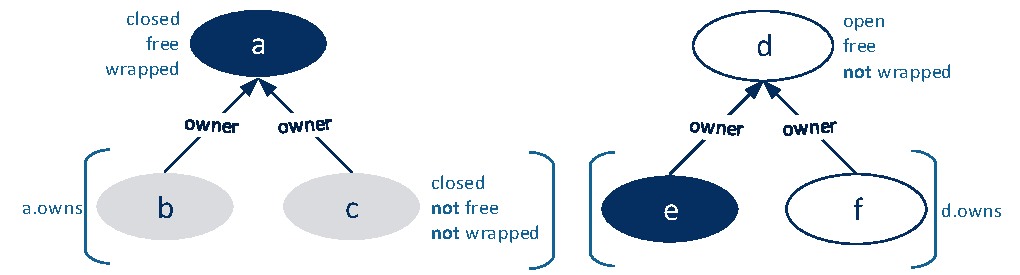
\includegraphics[width=\columnwidth]{images/objectstate.pdf}
\end{center}
\caption{Example of an object structure at run-time.} 
\label{fig:objectstate}
\end{figure}

We illustrate the possible object states on the example object structure of Figure~\ref{fig:objectstate}. The object structure consist of six objects:

\begin{itemize}
\item Object \e{a} is \emph{closed}, therefore its class invariant is guaranteed to hold. It does not have an owner and thus is \emph{free}. As it is both free and closed, it is also \emph{wrapped}. The object \e{a} owns the two objects \e{b} and \e{c}. This is defined through its \e{owns} set, i.e. \e{a.owns = \{b, c\}}.

\item Objects \e{b} and \e{c} are both owned by \e{a}, so their \e{owner} ghost field points to \e{a}. Since they are \emph{owned} they are \emph{not free}. As their owner \e{a} is \emph{closed}, the two objects \e{b} and \e{c} are \emph{closed} as well, as they are in \e{a}'s ownership domain.

\item Object \e{d} is \emph{open} and may potentially be in an inconsistent state, so its class invariant is not guaranteed to hold. It does not have an owner and is therefore \emph{free}. The object \e{d} owns the two objects \e{e} and \e{f}, defined through its \e{owns} set.

\item Object \e{e} is \emph{closed} and therefore consistent. Its owner is \e{d}, but since \e{d} is \emph{open}, \e{e} is considered to be \emph{free}. Being both \emph{closed} and \emph{free} means that \e{e} is \emph{wrapped}.

\item Object \e{f} is \emph{open} and potentially inconsistent. Analogous to \e{e} it is \emph{free}, as its owner \e{d} is \emph{open}.
\end{itemize}

The example illustrates the difference between ownership trees of \emph{open} and \emph{closed} objects. While ownership trees of consistent objects are guaranteed to be consistent as well---all objects in the ownership tree including the root object are \emph{closed}---, this property does not hold for ownership trees of potentially inconsistent objects. The ownership tree of an \emph{open} object may contain objects that are \emph{open} and objects that are \emph{closed}.


%===========================================================
\subsection{Object State Queries}
%===========================================================

\AutoProof offers ghost functions that can be used to query an object's state in assertions and specifications:

\begin{itemize}
\item \e{is_wrapped: BOOLEAN} -- is the object wrapped (closed and free)?
\item \e{is_free: BOOLEAN} -- is the object free (unowned or owner is open)?
\item \e{is_open: BOOLEAN}  -- is the object open (potentially inconsistent)?
\item \e{closed: BOOLEAN} -- is the object closed (consistent)?
\item \e{owner: ANY} -- owner of the object.
\item \e{owns: MML_SET [ANY]} -- set of owned objects.
\item \e{inv: BOOLEAN} -- does full invariant of the object hold?
\item \e{inv_only (t): BOOLEAN} -- does the invariant with tag \emph{t} hold?
\item \e{inv_without (t): BOOLEAN} -- does the invariant except for tag \emph{t} hold?
\end{itemize}

The last two functions \e{inv_only} and \e{inv_without} allow to reuse specification constructs. The argument to these functions is a list of manifest strings containing invariant tags. Given the class of Figure~\ref{code:tree_node} the condition that the \e{sequence} is consistent can be written as \e{inv_only ("sequence_def")}. This helps reduce the annotation burden for classes with comples class invariants.


%===========================================================
\subsection{Encoding Ownership}
%===========================================================

Ownership in \AutoProof is used by adding objects to and removing objects from the \e{owns} set. The usual way of doing this is by defining the \e{owns} set as part of the class invariant. The binary tree example has the following class invariant:
\begin{erunning}[numbers=none]
owns_def: owns = {like owns}[[left, right]] / Void
\end{erunning}
The owns set consists of the two objects \e{left} and \e{right} unless they are \e{Void}. As in other situations, the encoding of the \e{owns} set influences the ability of \AutoProof to reason about it. In the \e{maximum} function of the binary tree we have introduced two assertions \e{owns.has (left)} and \e{owns.has (right)} in the respective branches. Where we to remove these check instructions \AutoProof would fail in verifying the function (\emph{try it!}). 

This is due to the use of the set removal operation \e{/ Void}, which makes the reasoning about the set more difficult and forces us to help the verifier in the proof. Were we to use a different encoding of the \e{owns} set in the class invariant we could remove these assertions. The following encoding is more verbose but better suited for the verifier:
\begin{erunning}[basicstyle=\footnotesize]
owns =
	if left = Void then
		if right = Void then {like owns}[[]] else {like owns}[[right]] end
	else
		if right = Void then {like owns}[[left]] else {like owns}[[left, right]] end
	end
\end{erunning}
With this encoding there is no need for the intermediate check instructions anymore (\emph{try it!}).

%===========================================================
\subsection{Wrapping and Unwrapping} \label{sec:wrapping}
%===========================================================

The two ghost procedures \e{wrap} and \e{unwrap} are used to change an object from being \emph{unwrapped} to being \emph{wrapped} and vice versa. Figure~\ref{fig:wrapunwrap} gives an overview of how the object consistency changes when these procedures are called. 

\begin{figure}[!htb]
\begin{center}
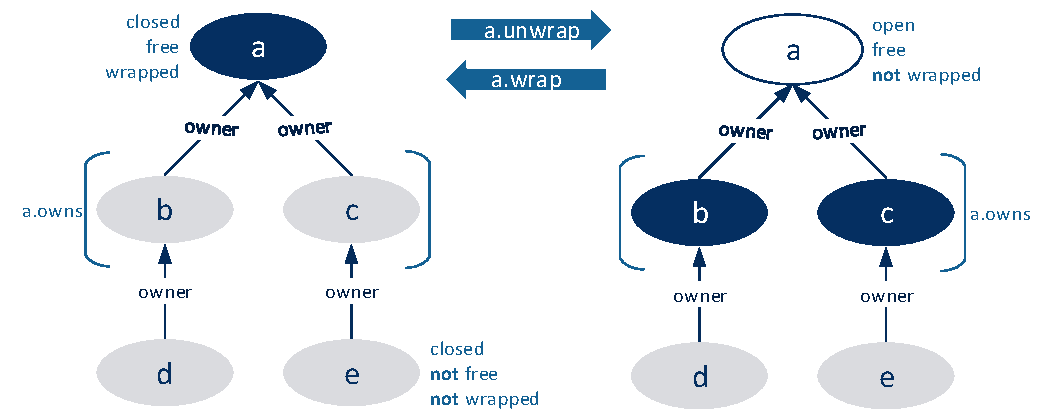
\includegraphics[width=\columnwidth]{images/wrapunwrap.pdf}
\end{center}
\caption{Change of object state on wrapping and unwrapping.}
\label{fig:wrapunwrap}
\end{figure}

Since wrapping and unwrapping changes the boolean ghost field \e{closed}, that field must be writable when either of these procedures are called. This is also the reason we had to add the field \e{closed} to the modifies clause in the \e{withdraw} procedure of the \emph{account} example (see Section~\ref{sec:framing}).

\e{wrap} and \e{unwrap} are axiomatized in the background theory of the verifier. Their definition in the class \e{ANY} does therefore not reflect their real semantics. The actual specification for \e{wrap} and \e{unwrap} could be written as follows:

\noindent\begin{tabular}{ll}
{\begin{erunning}[basicstyle=\scriptsize,numbers=left]
wrap
		-- Wrap `Current'.
	require
		is_open
		inv
		across owns as o all o.item.is_wrapped end
		modify_field ("closed", Current)
		modify_field ("owner", owns)
	ensure
		is_wrapped
		across owns as o all o.item.owner = Current end
	end
\end{erunning}}
&
\hspace{4mm}
{\begin{erunning}[basicstyle=\scriptsize,numbers=left,firstnumber=last]
unwrap
		-- Unwrap `Current.
	require
		is_wrapped
		modify_field ("closed", Current)
	ensure
		is_open
		across owns as o all 
		       o.item.is_wrapped end
	end
\end{erunning}}
\end{tabular}


%----------------------------------------------
\subsection{Defaults}
%----------------------------------------------

\AutoProof uses implicit default contracts, default wrapping, and default assignments of ghost fields to remove the annotation burden. The default contracts and wrapping depend on type and visibility of routines. The default assignment to ghost fields depends on their definition.

\paragraph{Creation routines} require by default that all arguments are wrapped. In addition, the \e{Current} object will be implicitly wrapped at the end of the routine body and the postcondition will assert that \e{Current} is wrapped.
\begin{erunning}
make ($args$)
	require
		$\forall o\in args : o$.is_wrapped
	do
		...
		Current.wrap
	ensure
		Current.is_wrapped
		$\forall o\in args : o$.is_wrapped
	end
\end{erunning}

\paragraph{Pure functions} can by default be called on \emph{closed} objects. It is therefore not necessary to unwrap the object before calling a function. Also there is no default postcondition since the objects are not mutated during the execution.
\begin{erunning}
pure_function ($args$): $type$
	require
		Current.is_closed
		$\forall o\in args : o$.is_closed
	do ...	end
\end{erunning}

\paragraph{Public procedures and public impure functions} require by default that all objects are in a consistent state, as they are callable from client code.
\begin{erunning}
public_procedure ($args$)
	require
		Current.is_wrapped
		$\forall o\in args : o$.is_wrapped
	do
		Current.unwrap
		...
		Current.wrap
	ensure
		Current.is_wrapped
		$\forall o\in args : o$.is_wrapped
	end
\end{erunning}

\paragraph{Private procedures and private impure functions} are only callable from a restricted set of clients, for example from the class itself. Since all public routines by default unwrap the \e{Current} object, private routines by default assume the object to be open.
\begin{erunning}
private_procedure ($args$)
	require
		Current.is_open
	do ...
	ensure
		Current.is_open
	end
\end{erunning}

\paragraph{Ghost fields} that have a definition in the class invariant of the form \e{$fieldname$ = $expression$} will be assigned implicitly every time the object is wrapped. This is the reason that the two ghost fields \e{owns} and \e{sequence} of the binary tree example are never explicitly assigned. \AutoProof assigns these fields implicitly at the end of each procedure when the implicit call to \e{wrap} takes place.

\paragraph{Functional functions} are often used in contracts and class invariants. Therefore they may operate on inconsistent objects and have no default preconditions.

%----------------------------------------------
\subsubsection*{Disabling Defaults}
%----------------------------------------------

It is possible to disable defaults by adding the following \e{note} clauses to routines and classes:
\begin{itemize}
\item \e{explicit: contracts} -- disable default pre- and postcondition; applicable to a routine or a class.
\item \e{explicit: wrapping} -- disable default \e{unwrap} and \e{wrap} instructions; applicable to a routine or a class.
\item \e{explicit: $\ fieldname$} -- disable default assignment to field $fieldname$ before wrapping; applicable to a class.
\end{itemize}

%===========================================================
\subsection{Modification of Owned Objects}
%===========================================================

Modifies clauses define a set of modifiable objects. Whenever an object is modifiable then the \emph{transitive closure} of all owned objects is also modifiable. It is therefore not necessary to add owned objects to a modifies clause when the owner is modifiable. A modifies clause of \e{modify (o)} is sufficient to potentially modify objects owned by \e{o}. Modifications of owned objects still require that the modified object is unwrapped.

%===========================================================
\subsection{Hands-On: Ring Buffer}
%===========================================================

The next exercise is about implementing a ring buffer backed by an array. This will highlight how to use ownership and model-based contracts to design a data structure.

\begin{enumerate}[label=\bfseries Task \arabic*:, leftmargin=1.8cm]
\item Add ownership definition for the \e{data} array to the class invariant.
\item Add class invariants for the bounds of \e{start} and \e{free}.
\item Add the model fields, model declaration, and class invariant describing the model.
\item Add the specifications to the routines of \e{RING_BUFFER}. The tests in the test class can help you to get the specification right. \\
      You should be able to verify both classes completely.
\end{enumerate}




\imagechapter
%############################################################################
\chapter{\AutoProof Manual}
\label{sec:ap-manual}
\chapterimage{images/manual}
%############################################################################

    This manual describes how to use \AutoProof. \AutoProof is an auto-active verifier for the 
    Eiffel programming language that can prove functional correctness of Eiffel programs annotated with contracts.
	\AutoProof is available as part of the Eiffel Verification Environment (EVE) or via an online version.

The manual is also available online:
\begin{center}
\url{http://se.inf.ethz.ch/research/autoproof/manual}.
\end{center}


%============================================================================
\section{\AutoProof in EVE}
%============================================================================

    AutoProof is integrated in \EVE, a research branch of EiffelStudio.

\subsubsection{Installation}

    Follow the installation instructions of \EVE\footnote{\url{http://se.inf.ethz.ch/research/eve}}.

\subsubsection{Open Project}

    Open and compile an EiffelStudio project using the EVE base library. For this you can download the example project provided\footnote{\url{http://se.inf.ethz.ch/research/autoproof/manual/template.zip}}. Launch EVE using the \emph{run\_eve} script in the EVE delivery and add the example's ecf file using the \emph{add project} button. When you have added the project you can open and compile it.


\subsubsection{Open \AutoProof tool panel}

    Click the menu entry \emph{View > Tools > AutoProof}. This will show the \AutoProof panel, which can be docked like the other tools in EVE.

\subsubsection{Run \AutoProof}

    The Eiffel compilation of the project has to be finished and successful in order to run \AutoProof. It is not necessary to do the C compilation when working with \AutoProof. When the project is compiled successfully, there are three ways to launch AutoProof:

  \begin{itemize}
    \item You can run \AutoProof using the \emph{Verify} button. By default, \AutoProof will verify the class or cluster that is shown in the editor pane. You can change this behavior by clicking the down-arrow on the \emph{Verify} button and select either to verify the parent cluster of the item currently shown in the editor, or to verify the whole system (excluding libraries).
    \item You can pick-and-drop a feature, class, or cluster onto the \emph{Verify} button.
    \item You can right-click a feature or class, and select \emph{Verify with AutoProof} in the context menu.
  \end{itemize}

    Only one execution of \AutoProof can run at a time, so when the verification has started the \emph{Verify} button will become inactive.

\subsubsection{Stop \AutoProof}

    When \AutoProof is running you can stop it using the red stop button next to the \emph{Verify} button. This can be helpful if you want to cancel a long-running verification.

\subsubsection{Filtering Results}

    There are two ways of filtering the results displayed by AutoProof:

  \begin{itemize}
    \item The three toggle-buttons can be used to show or hide all successful results, failed verifications, or semantic errors.
    \item The filter box can be used to enter a text. Only results will be shown where this text is contained in either the class name, feature name, or text message. To clear the filter box you can click the red \emph{x} button next to it.
  \end{itemize}

\subsubsection{Options}

    On the top-right of the \AutoProof tool is the options button. Clicking it will display the available options and if the option is enabled or disabled. Clicking any of the options will toggle its value. For an explanation of the options see the AutoProof Options Section~\ref{manual:options}.


%============================================================================
\section{\AutoProof on the Command-line}
%============================================================================

    The command-line version of \AutoProof is available as part of EVE.

\subsubsection{Run \AutoProof}

    To run \AutoProof via the command-line you have to run the EVE command-line compiler with a valid Eiffel project and add the \emph{-autoproof} option: 

\begin{erunning}
  ec.exe -config #\emph{ecf-file}# -target #\emph{ecf-target}# -autoproof
\end{erunning}


    By default all user classes in the system are verified by \AutoProof. To select which classes or routines are verified, you can add the class names and routine names as additional command-line arguments. The routine name is composed of the class name together with the routine in the format \e{CLASS.routine}.

\subsubsection{Options}

    \AutoProof has the same options on the command-line as for the graphical version. The available command-line options are listed in the \AutoProof Options Section~\ref{manual:options}.


%============================================================================
\section{\AutoProof on the Web}
%============================================================================

    The online version of \AutoProof\footnote{\url{http://cloudstudio.ethz.ch/comcom/\#AutoProof}} is integrated in ComCom\footnote{\url{http://cloudstudio.ethz.ch/comcom/}}, an online interface to run command-line tools.

\subsubsection{Examples}

    Across the top of the \AutoProof interface on Comcom are different examples that can be selected. The examples can be adapted in the browser. To reload the original version, click the reload button on the top-right.

\subsubsection{Custom code}

    The last tab \emph{More \AutoProof} can be used to write your own code. In addition to writing your own code you can use command-line options on this tab. For a list of command-line options, see the \AutoProof Options Section~\ref{manual:options}.

\subsubsection{Run \AutoProof}

    To run \AutoProof, click the \emph{Run} button below the code area. The results will be shown in the box below the button. Note that changing the example will clear the results box. The verification time is limited to 2 minutes, you will get a result or a time-out message after that time.

\subsubsection{Limitations}

    The ComCom version of \AutoProof is limited to examples that consist only of one user-defined class. You can use the classes of the EVE version of EiffelBase in your code, in particular the ones defined in the \AutoProof base library\footnote{\url{http://se.inf.ethz.ch/research/autoproof/reference}}. It is not possible to add further libraries.


%============================================================================
\section{\AutoProof Options} \label{manual:options}
%============================================================================

    There are different options which influence the behavior of the AutoProof translation and execution as a whole, as opposed to annotations which only affect individual classes or features (see the Annotations Section~\ref{manual:annotations} for details). Table~\ref{tab:manual:options} lists these options. The command-line switches usually come in pairs: one switch turns the option on and the other turns it off.

\begin{sidewaystable}
\centering
\begin{tabular}{>{\bfseries}llp{3cm}p{9cm}}
\textbf{Option name} & \textbf{Default} & \textbf{CLI switch} & \textbf{Description} \\
\hline
Two-step & Disabled & -twostep \newline -notwostep & Use two-step verification when enabled. \\ 
\hline
Automatic inlining & Disabled & -autoinline \newline -noautoinline & Inline routines without postcondition automatically when enabled. \\ 
\hline
Automatic unrolling & Disabled & -autounroll \newline -noautounroll & Unroll loops without loop invariants automatically when enabled. \\ 
\hline
Postcondition predicates & Disabled & -postpredicate \newline -nopostpredicate & Generate postcondition predicates when enabled. \\ 
\hline
Overflow & Disabled & -overflow \newline -nooverflow & Check for integer overflows when enabled. \\ 
\hline
Generate triggers & Disabled & -trigger \newline -notrigger & Generates triggers for across expressions when enabled. \\ 
\hline
Arithmetic triggers & Disabled & -arithtrigger \newline -noarithtrigger & Uses arithmetic functions for triggers when enabled. \\ 
\hline
SC defaults & Enabled & -scdefaults \newline -noscdefaults & Use semantic collaboration defaults when enabled. \\ 
\hline
Bulk verification & Bulk & -bulk \newline -forked & Bulk: all routines are verified at the same time and the results are displayed at the end. \newline Forked: routines are verified in parallel and results are displayed when available. \\ 
\hline
Timeout &  & -timeout X & \emph{Command-line only} - Boogie timeout in seconds. \\ 
\hline
HTML output &  & -html & \emph{Command-line only} - Produce HTML output. \\ 
\hline

\end{tabular}
\caption{\AutoProof options for the graphical and command-line interface}
\label{tab:manual:options}
\end{sidewaystable}



%============================================================================
\section{Verification Process}
%============================================================================


\subsubsection{Modularity}

  \AutoProof does routine-level modular verification. Each routine is verified in isolation and only the interface of suppliers are considered during the verification of a routine. A program can only be considered fully verified if all routines are verified individually. By default \AutoProof only verifies user-written classes when a program is verified, referenced libraries should be verified separately.

\subsubsection{Creation routines}

  Creation routines in Eiffel double as regular routines and can be called on existing objects. Since routines behave differently depending on whether they are called as a creation routine, e.g. the class invariant is not checked on entry and all attributes are set to their default value for creation routines, these routines are verified twice with \AutoProof. The feedback of \AutoProof will list these routines twice specifying the context of the verification.

  
\subsubsection{Assumptions}

  It can be useful to temporarily assume a fact that the verifier should use. This helps in debugging failed verifications, e.g. by directing the verifier in a specific branch. You can write an assumption using a check instruction with the special tag \emph{assume}.

\begin{erunning}
check assume: False end
\end{erunning}

\subsubsection{Skipping classes or routines}

You can skip the verification of single routines or classes by adding a note clause.

\begin{erunning}
note
  status: skip
\end{erunning}
  


%============================================================================
\section{Language Support} \label{manual:lang-support}
%============================================================================

\definecolor{full}{HTML}{DDFFDD}
\definecolor{partial}{HTML}{FFFFDD}
\definecolor{none}{HTML}{FFDDDD}


  The programming language that \AutoProof supports is not exactly the standard Eiffel language. Some features of the Eiffel language are not supported, on the other hand custom annotations have been added to increase the expressiveness of the specification language. All custom annotations are valid syntax in standard Eiffel.

%\subsection*{Standard Eiffel Support}

  \AutoProof supports a large portion of the Eiffel language. When \AutoProof encounters code constructs it does not support, it will try to degrade in a correct but incomplete way in order to verify the surrounding program. In any case, a special message will be displayed. Here is a comprehensive list of supported and unsupported instructions, expressions, and language concepts.
The color coding represents the level of support for the construct: \colorbox{full}{green} represents full support, \colorbox{partial}{yellow} partial support, and \colorbox{none}{red} no support.


%----------------------------------------------------------------------------
\subsection{Instructions}
%----------------------------------------------------------------------------

\noindent
\begin{longtable}{|l|l|m{6.8cm}|}
\hline
\textbf{Name} & \textbf{Example} & \textbf{Comment} \\ \endhead  \hline

Assignment
\cellcolor{full} 
&
{\begin{erunning}
a := b
\end{erunning}}
&

\\ \hline

Call
\cellcolor{full}
&
{\begin{erunning}
a.f (x)
\end{erunning}}
&
The verification will check if \e{a} is not Void and if the precondition of \e{f} holds. Adding tag names to the preconditions of \e{f} improves the error reporting.
\\ \hline

Check
\cellcolor{full}
&
{\begin{erunning}
check
	tag: c
end
\end{erunning}}
&
The verification will check if the condition \e{c} holds. Adding a tag name improves the error reporting.
\\ \hline

Conditional
\cellcolor{full}
&
{\begin{erunning}
if c then
... 
else 
... 
end
\end{erunning}}
&
\\ \hline

Creation
\cellcolor{full}
&
{\begin{erunning}
create a.f(x)
\end{erunning}}
&
The verification will check if the precondition of \e{f} holds. Adding tag names to the preconditions of \e{f} improves the error reporting.\\ \hline

Debug
\cellcolor{full}
&
{\begin{erunning}
debug ... end
\end{erunning}}
&
\\ \hline

Inspect
\cellcolor{full}
&
{\begin{erunning}
inspect a
when x then ...
when y..z then ...
else ...
end
\end{erunning}}
&
\\ \hline

From loop
\cellcolor{full}
&
{\begin{erunning}
from ...
invariant
	tag1: i1
	tag2: i2
until c
loop ...
variant v end
\end{erunning}}
&
The verification will check if the invariants \e{i1} and \e{i2} hold after the (possibly empty) \e{from} block is executed and after every loop iteration. If a loop variant \e{v} or \e{decreases} annotation is provided then it is checked that the variant is non-negative and is reduced in every loop iteration. Adding tag names to the loop invariants improves the error reporting.
\\ \hline

Across loop
\cellcolor{none}
&
{\begin{erunning}
across a as c
loop ...
end
\end{erunning}}
&
Across loops can be expressed with from loops.
\\ \hline


Retry
\cellcolor{none}
&
{\begin{erunning}
retry
\end{erunning}}
&
The retry statement is only used in exception handling, which is not supported.
\\ \hline
\end{longtable}


%----------------------------------------------------------------------------
\subsection{Expressions} 
%----------------------------------------------------------------------------

\noindent
\begin{longtable}{|m{2.7cm}|l|m{6.2cm}|}
\hline
\textbf{Name} & \textbf{Example} & \textbf{Comment} \\ \endhead  \hline

Access
\cellcolor{full}
&
{\begin{erunning}
a
\end{erunning}}
&

\\ \hline

Across
\cellcolor{partial}
&
{\begin{erunning}
across set as c 
	all ... end
across 1 |..| 5 as c 
	some ... end
\end{erunning}}
&
Only specific container types are supported: MML types, \newline\e{INTEGER_INTERVAL},\newline \e{SIMPLE_ARRAY}, and \e{SIMPLE_LIST}.
\\ \hline

Address
\cellcolor{none}
&
{\begin{erunning}
#\$#
\end{erunning}}
&
The address operator is used to interoperate with external C code, which is not supported.
\\ \hline

Access
\cellcolor{full}
&
{\begin{erunning}
a
\end{erunning}}
&

\\ \hline

Call
\cellcolor{full}
&
{\begin{erunning}
a.f (x)
\end{erunning}}
&
The verification will check if \e{a} is not Void and if the precondition of \e{f} holds. Adding tag names to the preconditions of \e{f} improves the error reporting.
\\ \hline

Conditional
\cellcolor{full}
&
{\begin{erunning}
if c then x 
	else y end
\end{erunning}}
&
\\ \hline

Creation \newline \emph{(body)}
\cellcolor{full}
&
{\begin{erunning}
create {T}.f (x)
\end{erunning}}
&
The verification will check if the precondition of \e{f} holds. Adding tag names to the preconditions of \e{f} improves the error reporting.
\\ \hline

Creation \newline \emph{(contract)}
\cellcolor{none}
&
{\begin{erunning}
create {T}.f (x)
\end{erunning}}
&
The contracts have to be side-effect free, creating objects in the contract is not supported.
\\ \hline

Agents
\cellcolor{partial}
&
{\begin{erunning}
agent f
\end{erunning}}
&
\\ \hline

Manifest array \newline \emph{(body)}
\cellcolor{full}
&
{\begin{erunning}
<<a, b>>
\end{erunning}}
&
This syntax can be used to initialize \e{SIMPLE_ARRAY}, \e{MML_SET}, or \e{MML_SEQUENCE} entities.
\\ \hline

Manifest array \newline \emph{(contract)}
\cellcolor{partial}
&
{\begin{erunning}
<<a, b>>
\end{erunning}}
&
This syntax can be used to initialize \e{MML_SET} or \e{MML_SEQUENCE} entities. Otherwise it is not supported as contracts have to be side-effect free.
\\ \hline

Manifest string \newline \emph{(body)}
\cellcolor{partial}
&
{\begin{erunning}
"abc"
\end{erunning}}
&
AutoProof provides a special string class \e{V_STRING} which can be initialized with manifest strings.
\\ \hline

Manifest string \newline \emph{(contract)}
\cellcolor{none}
&
{\begin{erunning}
"abc"
\end{erunning}}
&
Not supported as contracts have to be side-effect free.
\\ \hline

Manifest tuple \newline \emph{(body)}
\cellcolor{full}
&
{\begin{erunning}
[a, b]
\end{erunning}}
&
This syntax can be used to initialize \e{TUPLE}s or \e{MML_SET} entities.
\\ \hline

Manifest tuple \newline \emph{(contract)}
\cellcolor{partial}
&
{\begin{erunning}
[a, b]
\end{erunning}}
&
This syntax can be used to initialize \e{MML_SET} entities. Otherwise it is not supported as contracts have to be side-effect free.
\\ \hline

Object test
\cellcolor{full}
&
{\begin{erunning}
attached {T} a
	as x
\end{erunning}}
&
This syntax can be used to initialize \e{MML_SET} entities. Otherwise it is not supported as contracts have to be side-effect free.
\\ \hline

Old
\cellcolor{full}
&
{\begin{erunning}
old a
\end{erunning}}
&
The old keyword can only be used in postconditions. For accessing the prestate in the routine body \AutoProof provides a special query \e{old_}.
\\ \hline

\end{longtable}


%----------------------------------------------------------------------------
\subsection{Library support and built-in types} 
%----------------------------------------------------------------------------

\noindent
\begin{longtable}{|m{2.7cm}|l|m{6.35cm}|}
\hline
\textbf{Name} & \textbf{Example} & \textbf{Comment} \\ \endhead  \hline

Boolean values
\cellcolor{full}
&
{\begin{erunning}
True
False
\end{erunning}} 
&
\\ \hline

Boolean \newline operations
\cellcolor{full}
&
{\begin{erunning}
a and b or c
a implies b xor c
\end{erunning}} 
&
\\ \hline

Integer values
\cellcolor{full}
&
{\begin{erunning}
1
-2
\end{erunning}} 
&
\\ \hline

Integer \newline arithmetic 
\cellcolor{full}
&
{\begin{erunning}
a + b - c
a * b // c
\end{erunning}} 
&
The handling of integers is based on the built-in capabilities of Boogie. AutoProof also checks arithmetic overflows (if enabled).
\\ \hline

Floating point \newline values
\cellcolor{partial}
&
{\begin{erunning}
1.3
-2.4
\end{erunning}} 
&
Floating point values are mapped to Boogie's \b{real} type. This is only an approximation of floating-point numbers.
\\ \hline

Floating point \newline arithmetic
\cellcolor{partial}
&
{\begin{erunning}
a + b - c
a * b // c
\end{erunning}} 
&
Floating point values are mapped to Boogie's \b{real} type. This is only an approximation of floating-point numbers.
\\ \hline

Character values
\cellcolor{full}
&
{\begin{erunning}
'c'
\end{erunning}} 
&
Characters are mapped to the integer code of the character.
\\ \hline

Character \newline operations
\cellcolor{partial}
&
{\begin{erunning}
a + b
c.to_upper
\end{erunning}} 
&
Only basic arithmetic on characters is supported.
\\ \hline

Strings
\cellcolor{partial}
&
{\begin{erunning}
"abc"
\end{erunning}} 
&
AutoProof provides a special string class \e{V_STRING} which can be initialized with manifest strings.
\\ \hline

Base library
\cellcolor{partial}
&
{\begin{erunning}
a: SIMPLE_ARRAY
a[1]
a.put (v, 3)
\end{erunning}} 
&
An array and a list class are provided specifically for the use in spe\-cification: \e{SIMPLE_ARRAY} and  \newline \e{SIMPLE_LIST}.
\\ \hline

\end{longtable}

  

%============================================================================
\section{Annotations}\label{manual:annotations}
%============================================================================
  
The following tables give a summary of the custom annotations supported by AutoProof. If you use the same tag name for multiple values, you can use either multiple note entries or a comma-separated list for the values. For example the following two declarations are equivalent:

\begin{tabular}{ll}
{\begin{erunning}
note
	status: skip, functional
 #\ #
\end{erunning}}
&
{\begin{erunning}
note
	status: skip
	status: functional
\end{erunning}}
\end{tabular}

%----------------------------------------------------------------------------
\subsection{Class Annotations}
%----------------------------------------------------------------------------

These annotation can be used in the \e{note} clause of a class.

\noindent
\begin{longtable}{|m{2.5cm}|l|m{6.05cm}|}
\hline
\textbf{Name} & \textbf{Example} & \textbf{Comment} \\ \endhead  \hline

Explicit &
{\begin{erunning}
explicit: "all"
\end{erunning}} &
Turn off all semantic collaboration defaults in the class.
\\ \hline

Explicit \newline Contracts &
{\begin{erunning}
explicit: contracts
\end{erunning}} &
Turn off all semantic collaboration default contracts in the class.
\\ \hline

Explicit Sets &
{\begin{erunning}
explicit: observers
explicit: subjects
explicit: owns
\end{erunning}} &
Turn off semantic collaboration default invariants for the mentioned sets.
\\ \hline

Explicit \newline Wrapping &
{\begin{erunning}
explicit: wrapping
\end{erunning}} &
Turn off all semantic collabora\-ti\-on default unwrapping and wrapping instructions in the class.
\\ \hline

Manual inv() &
{\begin{erunning}
manual_inv: True
\end{erunning}} &
If \e{True} then you need to insert manual \e{inv}, \e{inv_only}, and \e{inv_without} assertions in the code.
\\ \hline

Model &
{\begin{erunning}
model: f, g
\end{erunning}} &
List of model queries.
\\ \hline

Status: Skip &
{\begin{erunning}
status: skip
\end{erunning}} &
Skip verification of whole class.
\\ \hline

Theory &
{\begin{erunning}
theory: "file.bpl"
\end{erunning}} &
Include the specified theory file in the generated Boogie code.
\\ \hline

Type \newline Mapping &
{\begin{erunning}
maps_to: "t"
\end{erunning}} &
Map this class to the specified custom Boogie type.
\\ \hline

Type \newline Properties &
{\begin{erunning}
type_properties: "f"
\end{erunning}} &
Comma-separated list of Boogie functions that define the type properties for reference-type generic parameters.
\\ \hline

Type \newline Invariant &
{\begin{erunning}
where: "f"
\end{erunning}} &
Boogie function that defines the type invariant for this type.
\\ \hline

\end{longtable}
  

%----------------------------------------------------------------------------
\subsection{Feature Annotations}
%----------------------------------------------------------------------------

These annotation can be used in the \e{note} clause of a feature.

\noindent
\begin{longtable}{|m{2.5cm}|l|m{6cm}|}
\hline
\textbf{Name} & \textbf{Example} & \textbf{Comment} \\ \endhead  \hline

Explicit &
{\begin{erunning}
explicit: "all"
\end{erunning}} &
Turn off all semantic collaboration defaults in the feature.
\\ \hline

Explicit \newline Contracts &
{\begin{erunning}
explicit: contracts
\end{erunning}} &
Turn off semantic collaboration default contracts in the feature.
\\ \hline

Explicit \newline Wrapping &
{\begin{erunning}
explicit: wrapping
\end{erunning}} &
Turn off semantic collaboration default unwrapping and wrapping instructions in the feature.
\\ \hline

Function \newline Mapping &
{\begin{erunning}
maps_to: "f"
\end{erunning}} &
Map this feature to the specified Boogie function.
\\ \hline

Guard &
{\begin{erunning}
guard: True
guard: False
guard: "f"
\end{erunning}} &
Set the update guard of this attribute to the specified value. The update guard feature has to be \e{functional}.
\\ \hline

Inlining &
{\begin{erunning}
inline: True
inline: 4
\end{erunning}} &
Inline calls in this routine. If a number is given, then the calls will be inlined up to the specified depth.
\\ \hline

Manual inv() &
{\begin{erunning}
manual_inv: True
\end{erunning}} &
If set to true then you need to insert manual \e{inv}, \e{inv_only}, and \e{inv_without} assertions in the code.
\\ \hline

Status: \newline Creator &
{\begin{erunning}
status: creator
\end{erunning}} &
Verify this routine only in the context of a creation routine.
\\ \hline

Status: \newline Dynamic &
{\begin{erunning}
status: dynamic
\end{erunning}} &
Verify this routine assuming the \e{Current} type might be a subtype. This removes the need to reverify this routine in subclasses.
\\ \hline

Status: \newline Functional &
{\begin{erunning}
status: functional
\end{erunning}} &
Mark this routine as functional. Functional features can only contain a single instruction that assigns a value to the \e{Result}.
\\ \hline

Status: \newline Ghost &
{\begin{erunning}
status: ghost
\end{erunning}} &
Mark the feature as a ghost feature.
\\ \hline

Status: \newline Impure &
{\begin{erunning}
status: impure
\end{erunning}} &
Functions are supposed to have an empty modifies clause and are therefore pure. By marking a function as impure, you can add a modifies clause.
\\ \hline

Status: \newline Inline &
{\begin{erunning}
status: inline
\end{erunning}} &
Mark this feature to be always inlined in the caller.
\\ \hline

Status: \newline Lemma &
{\begin{erunning}
status: lemma
\end{erunning}} &
Mark this feature as a lemma. Lemma features have no automatic unwrapping and wrapping of the Current object and are implicitly ghost.
\\ \hline

Status: \newline Skip &
{\begin{erunning}
status: skip
\end{erunning}} &
Skip verification of this feature.
\\ \hline

\end{longtable}
	

%----------------------------------------------------------------------------
\subsection{Precondition and Loop Invariant Functions}
%----------------------------------------------------------------------------

These annotations are used in the precondition of features or the invariant clause of loops.

\noindent
\begin{longtable}{|m{1.9cm}|l|m{5.6cm}|}
\hline
\textbf{Name} & \textbf{Example} & \textbf{Comment} \\ \endhead  \hline

Decreases &
{\begin{erunning}
decreases (x)
decreases ([x, y])
decreases ([])
\end{erunning}} &
Specify the variant of a recursive function or a loop. An empty decreases clause (last line) removes the termination check entirely.
\\ \hline

Modifies \newline (object) &
{\begin{erunning}
modify (Current)
modify (set)
\end{erunning}} &
Allow this routine or loop to modify all attributes of the given objects.
\\ \hline

Modifies \newline (field) &
{\begin{erunning}
modify_field ("x", o)
modify_field ("x", set)
modify_field (["x", "y"], o)
\end{erunning}} &
Allow this routine or loop to modify the specified attributes of the given objects.
\\ \hline

Modifies \newline (model) &
{\begin{erunning}
modify_model ("x", o)
modify_model ("x", set)
modify_model (["x", "y"], o)
\end{erunning}} &
Allow this routine or loop to modify the specified models of the given objects.
\\ \hline

Reads &
{\begin{erunning}
reads (o)
reads_field ("attr", o)
reads_model ("attr", o)
\end{erunning}} &
Allow this functional routine to read the specified objects, attributes or models.
\\ \hline

\end{longtable}

%----------------------------------------------------------------------------
\subsection{Commands and Queries}
%----------------------------------------------------------------------------

These features are used in the regular body of routines.

\noindent
\begin{longtable}{|m{2.5cm}|l|m{6cm}|}
\hline
\textbf{Name} & \textbf{Example} & \textbf{Comment} \\ \endhead  \hline

Invariant &
{\begin{erunning}
inv
other.inv
\end{erunning}} &
Check whether the class invariant of an object holds.
\\ \hline

Partial \newline invariant &
{\begin{erunning}
inv_only ("t1", "t2")
o.inv_without ("t")
\end{erunning}} &
Check whether part of the class invariant holds. The check takes a list of tag names given by string constants and either just checks these tags (\e{inv_only}) or the whole invariant except for the specified tags (\e{inv_without}).
\\ \hline

Is Free &
{\begin{erunning}
is_free
other.is_free
\end{erunning}} &
Returns whether an object is free. Free objects have no owner.
\\ \hline

Is Fresh &
{\begin{erunning}
is_fresh
other.is_fresh
\end{erunning}} &
Returns whether an object is fresh. Fresh objects were not allocated in the pre-state.
\\ \hline

Is Open &
{\begin{erunning}
is_open
other.is_open
\end{erunning}} &
Returns whether an object is open. Open objects might not satisfy their class invariant.
\\ \hline

Is Wrapped &
{\begin{erunning}
is_wrapped
other.is_wrapped
\end{erunning}} &
Returns whether an object is wrapped. Wrapped objects are closed and free.
\\ \hline

Unwrapping &
{\begin{erunning}
unwrap
other.unwrap
unwrap_all (set)
\end{erunning}} &
Unwrap an object or a set of objects.
\\ \hline

Wrapping &
{\begin{erunning}
wrap
other.wrap
wrap_all (set)
\end{erunning}} &
Wrap an object or a set of objects.
\\ \hline

\end{longtable}



\normalchapter
\cleardoublepage
%\chapterimage{images/bibliography.jpg}

%\nocite{*}
\bibliographystyle{plain}
\bibliography{bibliography}


\normalchapter
\chapter*{Julian Tschannen}
\pagestyle{empty}

\vspace{-1cm}

\begin{tabbing}
Nationality: \hspace{1mm} \= Swiss \\
Date of birth: \> October 27, 1982 \\
Homepage:      \> \href{http://jt.x73.ch}{\texttt{jt.x73.ch}} \\
Email:         \> \href{mailto:jt@x73.ch}{\texttt{jt@x73.ch}} \\
\end{tabbing}


\section*{Work \& Education}

\begin{itemize}
  \item
  10/2009 -- 04/2015: \textbf{Dr. sc. ETH Zurich}, Switzerland\\
  Research assistant at the Chair of Software Engineering in the Department of Computer Science at ETH Zurich.

  \item
  10/2007 -- 04/2009: \textbf{MSc ETH in Computer Science}, Switzerland\\
  Degree with distinction, specialization in Software Engineering

  \item
  10/2006 -- 08/2007: \textbf{Internship at Eiffel Software}, USA

  \item
  10/2003 -- 10/2006: \textbf{BSc ETH in Computer Science}, Switzerland

\end{itemize}


\section*{Administrative \& Teaching Activities}

\begin{itemize}

  \item
  09/2010 -- 09/2014: \textbf{Organizer of LASER Summer School}\\
  I have co-organized the LASER summer school five times. The summer school is held in Elba, Italy.

  \item
  09/2012 -- 03/2015: \textbf{Project supervisor}\\
  I have supervised three lab projects, two Bachelor's theses, and one Master's thesis.

  \item
  09/2009 -- 12/2014: \textbf{Teaching assistant and Guest Lecturer}\\
  I have been head- or teaching assistant in nine courses and given various guest lectures.

\end{itemize}


\section*{Publications}

\begin{itemize}

  \item
  C. A. Furia, C. Poskitt, and J. Tschannen.
  \emph{The AutoProof Verifier: Usability by Non-Experts and on Standard Code}.
  In F-IDE, 2015.

  \item
  N. Polikarpova, J. Tschannen, and C. A. Furia.
  \emph{A Fully Verified Container Library}.
  In FM, 2015.

  \item
  J. Tschannen, C. A. Furia, M. Nordio, and N. Polikarpova. 
  \emph{AutoProof: Auto-active Functional Verification of Object-oriented Programs}.
  In TACAS, 2015

  \item
  N. Polikarpova, J. Tschannen, C. A. Furia, and B. Meyer.
  \emph{Flexible Invariants Through Semantic Collaboration}.
  In FM, 2014.

  \item
  J. Tschannen, C. A. Furia, and M. Nordio.
  \emph{AutoProof Meets Some Verification Challenges}.
  In STTT, 2014.

  \item
  J. Tschannen, C. A. Furia, M. Nordio, and B. Meyer.
  \emph{Program Checking With Less Hassle}.
  In VSTTE, 2013.

  \item
  J. Tschannen, C. A. Furia, M. Nordio, and B. Meyer.
  \emph{Automatic Verification of Advanced Object-Oriented Features: The AutoProof Approach}.
  In LASER: Tools for Practical Software Verification, 2012.

  \item
  T. Bormer, et al.
  \emph{The COST IC0701 Verification Competition 2011}.
  In FoVeOos, 2011.

  \item
  J. Tschannen, C. A. Furia, M. Nordio, and B. Meyer.
  \emph{Usable Verification of Object-Oriented Programs by Combining Static and Dynamic Techniques}.
  In SEFM, 2011.

  \item
  J. Tschannen, C. A. Furia, M. Nordio, and B. Meyer.
  \emph{Verifying Eiffel Programs with Boogie}.
  In BOOGIE, 2011.

  \item
  M. Nordio, H.-C. Estler, B. Meyer, J. Tschannen, C. Ghezzi, and E. Di Nitto.
  \emph{How do Distribution and Time Zones affect Software Development? A Case Study on Communication}.
  In ICGSE, 2011.

  \item
  M. Nordio, C. Ghezzi, B. Meyer, E. Di Nitto, G. Tamburrelli, J. Tschannen, N. Aguirre, and V. Kulkarni,
  \emph{Teaching Software Engineering using Globally Distributed Projects: the DOSE course}.
  In CTGDSD, 2011.

  \item
  M. Nordio, C. Calcagno, B. Meyer, P. M\"uller, and J. Tschannen.
  \emph{Reasoning about Function Objects}.
  In TOOLS-EUROPE, 2010.

\end{itemize}


\end{document}
